\documentclass{article}

% if you need to pass options to natbib, use, e.g.:
% \PassOptionsToPackage{numbers, compress}{natbib}
% before loading neurips_2020

% ready for submission
\usepackage[final,nonatbib]{neurips_2020}

% to compile a preprint version, e.g., for submission to arXiv, add add the
% [preprint] option:
%     \usepackage[preprint]{neurips_2020}

% to compile a camera-ready version, add the [final] option, e.g.:
%     \usepackage[final]{neurips_2020}

% to avoid loading the natbib package, add option nonatbib:
%     \usepackage[nonatbib]{neurips_2020}

\usepackage[utf8]{inputenc} % allow utf-8 input
\usepackage[T1]{fontenc}    % use 8-bit T1 fonts
\usepackage{amsmath}
\usepackage{hyperref} % hyperlinks
\usepackage{cleveref}
\crefformat{footnote}{#2\footnotemark[#1]#3}

\usepackage{url}            % simple URL typesetting
\usepackage{booktabs}       % professional-quality tables
\usepackage{amsfonts}       % blackboard math symbols
\usepackage{nicefrac}       % compact symbols for 1/2, etc.
\usepackage{microtype}      % microtypography
\usepackage{xcolor}

\usepackage{bm}
\usepackage{amsthm}
\usepackage{amssymb}
\usepackage{amsfonts}
\usepackage{graphicx}
\usepackage{makecell}
\usepackage{multirow}

\theoremstyle{definition}

\newtheorem{theorem}{Theorem}
\newtheorem{proposition}{Proposition}
\newtheorem{definition}{Definition}
\newtheorem{remark}{Remark}
\newtheorem{example}{Example}


% \newcommand{\todo}[1]{\textcolor{red}{#1}}
\newcommand{\todo}[1]{}

\newcommand{\mbf}[1]{\mathbf{#1}}
\newcommand{\mcl}[1]{\mathcal{#1}}
\newcommand{\mbb}[1]{\mathbb{#1}}

\newcommand{\da}{\mcl{D}}
\newcommand{\dc}{\mcl{D}_r}
\newcommand{\dr}{\mcl{D}_e}
%\newcommand{\da}{\mcl{D}_{\text{+}}}
%\newcommand{\dc}{\mcl{D}}
%\newcommand{\dr}{\mcl{D}_{\text{-}}}

%\newcommand{\elbo}{u_{\hspace{0.3mm}\text{\textless}}}
%\newcommand{\eubo}{u_{\hspace{0.3mm}\text{\textgreater}}}
%\newcommand{\elbo}{u_{{\scriptscriptstyle{\mathcal{L}}}}}
%\newcommand{\eubo}{u_{{\scriptscriptstyle{\mathcal{U}}}}}
\newcommand{\eubo}{\tilde{q}_u}
\newcommand{\elbo}{\tilde{q}_v}

\title{Variational Bayesian Unlearning}

% The \author macro works with any number of authors. There are two commands
% used to separate the names and addresses of multiple authors: \And and \AND.
%
% Using \And between authors leaves it to LaTeX to determine where to break the
% lines. Using \AND forces a line break at that point. So, if LaTeX puts 3 of 4
% authors names on the first line, and the last on the second line, try using
% \AND instead of \And before the third author name.

\author{%
  Quoc Phong Nguyen, Bryan Kian Hsiang Low, and Patrick Jaillet\textsuperscript{\dag}\\
  Dept. of Computer Science, National University of Singapore, Republic of Singapore\\
  Dept. of Electrical Engineering and Computer Science, MIT, USA\textsuperscript{\dag}\\
  \texttt{\{qphong,lowkh\}@comp.nus.edu.sg}, \texttt{jaillet@mit.edu}\textsuperscript{\dag}
%  Quoc Phong Nguyen \\
%  School of Computing\\
%  National University of Singapore
%  \And
%  Kian Hsiang Low\\
%  School of Computing\\
%  National University of Singapore\\
%  \And
%  Patrick Jaillet\\
%  Department of Electrical Engineering and Computer Science\\
%  Massachusetts Institute of Technology
%  David S.~Hippocampus\thanks{Use footnote for providing further information
%    about author (webpage, alternative address)---\emph{not} for acknowledging
%    funding agencies.} \\
%  Department of Computer Science\\
%  Cranberry-Lemon University\\
%  Pittsburgh, PA 15213 \\
%  \texttt{hippo@cs.cranberry-lemon.edu} \\
  % examples of more authors
  % \And
  % Coauthor \\
  % Affiliation \\
  % Address \\
  % \texttt{email} \\
  % \AND
  % Coauthor \\
  % Affiliation \\
  % Address \\
  % \texttt{email} \\
  % \And
  % Coauthor \\
  % Affiliation \\
  % Address \\
  % \texttt{email} \\
  % \And
  % Coauthor \\
  % Affiliation \\
  % Address \\
  % \texttt{email} \\
}

\begin{document}

\maketitle

\begin{abstract}
This paper studies the problem of approximately unlearning a Bayesian model from a small subset of the training data to be erased. We frame this problem as one of minimizing the Kullback-Leibler divergence between the approximate posterior belief of model parameters after directly unlearning from erased data vs.~the exact posterior belief from retraining with remaining data. Using the \emph{variational inference} (VI) framework, we show that it is equivalent to minimizing an evidence upper bound which trades off between fully unlearning from erased data vs.~not entirely forgetting the posterior belief given the full data (i.e., including the remaining data); the latter prevents catastrophic unlearning that can render the model useless. In model training with VI, only an approximate (instead of exact) posterior belief given the full data can be obtained, which makes unlearning even more challenging. We propose two novel tricks to tackle this challenge. We empirically demonstrate our unlearning methods on Bayesian models such as sparse Gaussian process and logistic regression using synthetic and real-world datasets.%\vspace{-1mm}
%from a posterior belief obtained by training a model exactly with Bayesian inference, or approximately with \emph{variational inference} (VI). By framing the unlearning as a minimization problem of a Kullback-Leibler divergence, we propose two different solutions, one of which can be interpreted as a counterpart of the evidence lower bound in the conventional VI. These methods are further endowed with an adjusted likelihood to mitigate the undesired effect of unlearning from an approximate posterior belief.
\end{abstract}

\todo{measure -> criterion ->  the existence of the opposite -> leads to learn vs unlearn (ELBO vs EUBO)}

\section{Introduction}
\label{sec:intro}
%prevalent and deeply intertwined into our daily lives
%Machine learning is now prevalently used in our daily life such that they ingest large quantities of user data for training.
%The advent of machine learning has brought about a significant improvement in our quality of life.
Our interactions with \emph{machine learning} (ML) applications have surged in recent years 
%Machine learning applications have now become prevalent in our daily life. 
such that large quantities of users' data are now deeply ingrained into the ML models being trained for these applications.
%As machine learning interweaves deeply into the daily life, a large amount of user information is continuously ingrained into many machine learning models. 
%Although this improves the life quality significantly,
%It is thus challenging 
%This complicates our ability 
This greatly complicates the regulation of access to each user's data or implementation of  \emph{personal data ownership}, which are enforced by the General Data Protection Regulation in the European Union~\cite{mantelero2013eu}.
In particular, 
%it would be desirable 
if a user would like to exercise her \emph{right to be forgotten}~\cite{mantelero2013eu} (e.g., when quitting an ML application),
then it would be desirable to have the trained ML model  ``unlearn'' from her data.
Such a problem of \emph{machine unlearning}~\cite{cao2015towards} extends to the practical scenario where a small subset of data previously used for training is later identified as malicious (e.g., anomalies)~\cite{cao2015towards,du2019lifelong} and the trained ML model can perform well once again if it can unlearn from the malicious data.

A naive alternative to machine unlearning is to simply retrain an ML model from scratch with the data \emph{remaining} after \emph{erasing} that to be unlearned from.
%\emph{remaining} data (i.e.,  the \emph{full} data except that to be unlearned from or \emph{erased}). 
In practice, this is prohibitively expensive in terms of time and space costs since the remaining data is often large such as in the above scenarios.
How then can a trained ML model  \emph{directly} and efficiently unlearn from a small subset of data to be erased to become (a) exactly and if not, (b) approximately close to that from retraining with the large remaining data?
Unfortunately, (a) exact unlearning is only possible for selected ML models (e.g., naive Bayes classifier, linear regression, $k$-means clustering, and item-item collaborative filtering \cite{cao2015towards,ginart2019making,schelteramnesia}).
This motivates the need to consider (b) approximate unlearning as it is applicable to a broader family of ML models like neural networks  \cite{du2019lifelong,golatkar2019eternal} but, depending on its choice of loss function, may suffer from \emph{catastrophic unlearning}\footnote{\label{beef}A trained ML model is said to experience \emph{catastrophic unlearning} from the erased data when its resulting performance is considerably worse than that from retraining with the remaining data.} that can render the model useless.
For example, to mitigate this issue, 
%
%to yield a much poorer performance than that from retraining with the remaining data.
%
%can potentially suffer from \emph{catastrophic unlearning}
the works of~\cite{du2019lifelong,golatkar2019eternal} have to ``patch up''
%introduce additional modifications of 
their loss functions by additionally bounding the loss incurred by erased data with a rectified linear unit and injecting a regularization term to retain information of the remaining data, respectively.
This begs the question whether there exists a loss function that can \emph{directly} quantify the approximation gap
and \emph{naturally} prevent catastrophic unlearning.

%in turn entails the issue of  to be addressed.

%However, since unlearning is only performed approximately using only the removed data in the latter approach, it is challenging to avoid the \emph{catastrophic unlearning} issue, i.e., unlearning the removed data affects the performance on the remaining data.
%It often requires extra modification of the unlearning objective. The work of \cite{du2019lifelong} maximizes the loss of the removed data wrapped in a rectified linear unit to enforce a bounding value. The work of \cite{golatkar2019eternal} introduces an additional regularization term to retain the information of the remaining data. 
%These works trigger our curiosity about whether there exists an unlearning objective that naturally removes the information of the removed data while still retaining that of the remaining data.

%Hence, it is desirable (and technically more challenging) to develop an efficient methodology for the trained ML model to \emph{directly} unlearn from the small subset of data to be erased.

%by ``undoing'' the effect of training with her data from the ML model
%removing her contribution of data from a trained ML model
%Towards the perspective of a personal data economy, we would like to fulfill the inevitable desire of a user: removal of his/her data from a model (e.g., when he/she stops using an application).
%Such a problem is known as \emph{machine unlearning} where the model unlearns from 

%removes a subset of the \emph{full} training data (i.e., \emph{removed data}) from a trained ML model~\cite{cao2015towards}. 
% The need was materialized into legislation, e.g., the so-called ``right to be forgotten'' in the General Data Protection Regulation in the European Union \cite{mantelero2013eu}, which further emphasizes its significance.
%From a utility viewpoint, machine unlearning can also be used to eliminate the undesirable effects of incorrect/malicious data (i.e., anomalies) from a model \cite{cao2015towards,du2019lifelong}.
%Yet, this process is challenging due to the constraints on the computational time and the 
%%%%% approximation in the training of the model.
%For example, the na\"ive method of re-training the model from scratch with the \emph{remaining data} (i.e., the full training data excluding the removed data) often incurs too much time to be practical due to the large amount of the remaining data. 
%%%%% Intuitively, the information of the remaining data is contained in the current trained model, 
%so machine unlearning often uses the current trained model and the removed data (which is often much less than the remaining data) \cite{cao2015towards}.

%The above constraints, especially unlearning with only the removed data to obtain the same model as that from re-training, are not feasible for all machine learning models.
%While there are models capable of being unlearned exactly (i.e., producing the same model as that from re-training) with only the removed data, e.g., na\"ive Bayes classifier, linear regression, the k-means clustering algorithm, item-item collaborative filtering \cite{cao2015towards,ginart2019making,schelteramnesia},
%unlearning methods that are capable of unlearning approximately (i.e., producing a model that is close to that from re-training) begin gaining interest due to its application to a broader family of machine learning methods, e.g., neural networks  \cite{du2019lifelong,golatkar2019eternal}.
%However, since unlearning is only performed approximately using only the removed data in the latter approach, it is challenging to avoid the \emph{catastrophic unlearning} issue, i.e., unlearning the removed data affects the performance on the remaining data.
%It often requires extra modification of the unlearning objective. The work of \cite{du2019lifelong} maximizes the loss of the removed data wrapped in a rectified linear unit to enforce a bounding value. The work of \cite{golatkar2019eternal} introduces an additional regularization term to retain the information of the remaining data. These works trigger our curiosity about whether there exists an unlearning objective that naturally removes the information of the removed data while still retaining that of the remaining data.

\nocite{bourtoule2019machine}

% Given the imperative for machine unlearning, there are several works that unlearn different types of models. The pioneer work is about unlearning models that depend on a summation of a small number of terms \cite{cao2015towards}, e.g., item-item collaborative filtering, na\"ive Bayes classifier, and the k-means clustering algorithm. Some of these models are also studied in \cite{schelteramnesia}. The work of \cite{ginart2019making} introduces the notion of deletion efficiency by posing the data deletion problem (i.e., machine unlearning) in the context of online learning. They propose two unlearning algorithms for the k-means clustering algorithm that can achieve the deletion efficiency.
% Inspired from the differential privacy, another work introduces the definition of certified removal for an algorithm \cite{guo2019certified}.
% linear/nonlinear logistic regression
% \cite{golatkar2019eternal} based on KL divergence.
% \cite{schelteramnesia} says that it is challenging for gradient descent algorithm as each step of the gradient descent depends on all data points (or a random batch) and the previous updated parameters.
% \cite{du2019lifelong} for anomaly detection

% In this paper, we aim to unlearn a Bayesian model by first investigating the question whether we can perform unlearning with the trained model (i.e., the posterior belief of the model parameters given the training data) and only the removed data (instead of the remaining data) in Sec.~\ref{subsec:exactbayesunlearn}. Fortunately, the answer is affirmative when the data are conditionally independent given the model parameters and the exact posterior belief of the model parameters is available.

Our work here addresses the above question by focusing on the family of Bayesian models.
Specifically, our proposed loss function measures the \emph{Kullback-Leibler} (KL) divergence between the approximate posterior belief of model parameters by directly unlearning from erased data vs.~the exact posterior belief from retraining with remaining data. Using the \emph{variational inference} (VI) framework, we show that minimizing this KL divergence is equivalent to \emph{minimizing} (instead of maximizing) a counterpart of the evidence lower bound called the \emph{evidence upper bound} (EUBO) (Sec.~\ref{subsec:exactfull}). Interestingly, the EUBO lends itself to a natural interpretation of a trade-off between fully unlearning from erased data vs.~not entirely forgetting the posterior belief given the \emph{full} data (i.e., including the remaining data); the latter prevents catastrophic unlearning induced by the former.

%we are particularly interested in the \emph{variational inference} (VI) framework for Bayesian models. It is because the objective function of VI is the \emph{evidence lower bound} (ELBO) which comprises of a term to maximize the likelihood of the data and the other term to retain the information from the prior belief. Furthermore, VI has a principled foundation since maximizing ELBO is interpreted as minimizing a \emph{Kullback-Leibler} (KL) divergence that quantifies the approximation quality. It is this remote resemblance between ELBO and our above thoughts on the unlearning objective poses a question that whether a counterpart of ELBO exists for unlearning. Fortunately, the answer is affirmative as described in Sec.~\ref{subsec:exactfull} given an exact posterior belief of the full training data.

% Given the exact posterior belief of the model parameters and the required data, we propose an \emph{evidence upper bound} (EUBO) to unlearn a Bayesian model in Sec.~\ref{subsec:exactfull}. It is capable of producing an approximate posterior belief of the model parameters given the remaining data (i.e., the approximate \emph{unlearned posterior belief}) that minimizes the \emph{Kullback-Leibler} (KL) divergence to that obtained by re-training the model with the remaining data.

Often, in model training, only an approximate (instead of exact) posterior belief of model parameters given the full data can be learned, say, also using VI. This makes unlearning even more challenging.
%: For example, suppose that the exact posterior belief is bimodal, i.e., it consists of modes $\mcl{A}$ and $\mcl{B}$. The approximate posterior belief can only capture one mode, say, $\mcl{A}$. 
%If the likelihood of the erased data is only high at mode $\mcl{B}$, then unlearning from  erased data should hardly change the approximate posterior belief  concentrated at mode $\mcl{A}$.
%of the exact posterior belief which is a bimodal distribution ().
To tackle this challenge, we analyse two sources of inaccuracy in the approximate posterior belief learned using VI, which lay the groundwork for proposing our first trick of an \emph{adjusted likelihood} of erased data (Sec.~\ref{subsubsec:eubo}): %reduce the effect of 
Our key idea is to curb
unlearning in the region of model parameters with low  approximate posterior belief where both sources of inaccuracy primarily occur.
%differs from the exact one.
% By tuning the adjusted likelihood, the unlearning region of the model parameters can be controlled.
Additionally, to avoid the risk of incorrectly tuning the adjusted likelihood, we propose another trick of \emph{reverse KL}  (Sec.~\ref{subsubsec:rkl}) which is naturally more protected from such inaccuracy without needing the adjusted likelihood. Nonetheless, our adjusted likelihood is general enough to be applied to reverse KL. 

%VI is a popular method to learn an approximate posterior belief of many Bayesian models thank to its scalability to large dataset \cite{hoang2015unifying}, and its modeling with complex posterior beliefs using generative adversarial networks \cite{yu19} and normalizing flows \cite{kingma2016improved,rezende2015variational}. 

VI is a popular approximate Bayesian inference framework due to its scalability to massive datasets~\cite{hensman2013gaussian,hoang2015unifying} and its ability to model complex posterior beliefs using generative adversarial networks \cite{yu19} and normalizing flows \cite{kingma2016improved,rezende2015variational}. 
Our work in this paper exploits VI to broaden the family of ML models that can be unlearned, which we empirically demonstrate using synthetic and real-world datasets on several Bayesian models such as sparse Gaussian process and logistic regression with the approximate posterior belief modeled by a normalizing flow (Sec.~\ref{sec:experiment}).%\vspace{-1mm}
%
% Although it is an interesting result that EUBO is a counterpart of the \emph{evidence lower bound} (ELBO) in the conventional \emph{variational inference} (VI), EUBO relies on the exact posterior belief of the model parameters given all the training data which is hardly available. In practice, only an approximate posterior belief of the model parameters is available. In particular, we focus on the case that training the model is performed with VI \cite{blei2017variational}.
% It is a popular solution to learn an approximate posterior belief thanks to several benefits: VI can be formulated as an anytime algorithm which is scalable to large dataset \cite{hoang2015unifying}; VI can be incorporated with generative models such as generative adversarial networks \cite{yu19} and normalizing flows (e.g., inverse autoregressive flows) \cite{rezende2015variational,kingma2016improved} to model complex posterior beliefs.
%
% Although it is an interesting result that EUBO is a counterpart of the \emph{evidence lower bound} (ELBO) in the conventional \emph{variational inference} (VI), EUBO relies on the exact posterior belief of the model parameters given all the training data which is hardly available. In practice, only an approximate posterior belief of the model parameters is available. In particular, we focus on the case that training the model is performed with VI \cite{blei2017variational}.
% It is a popular solution to learn an approximate posterior belief thanks to several benefits: VI can be formulated as an anytime algorithm which is scalable to large dataset \cite{hoang2015unifying}; VI can be incorporated with generative models such as generative adversarial networks \cite{yu19} and normalizing flows (e.g., inverse autoregressive flows) \cite{rezende2015variational,kingma2016improved} to model complex posterior beliefs.
%
% In contrast to the popularity of VI, unlearning Bayesian models trained with VI is challenging due to the approximation in the posterior belief. In particular, directly applying our proposed EUBO approach may lead to an undesired outcome.
% For example, the approximate posterior belief (of the model parameters) may capture only one mode of the exact posterior belief which is a multimodal distribution.
% Then, the question whether unlearning the removed data changes the approximate posterior belief significantly depends on whether the likelihood of removed data is large at the mode captured by the approximate posterior belief or not: if this likelihood is only large at the mode that is not captured by the approximate posterior belief, unlearning the removed data should not change the approximate posterior belief much.
%
% To resolve the above issue, we analyse two sources of inaccuracy in the approximate posterior belief obtained with VI which lays the foundation of our adjusted likelihood in Sec.~\ref{subsubsec:eubo}. The key idea is to reduce the unlearning effect on the region of the model parameters where the approximate posterior belief is different from the exact posterior belief (of the model parameters).
% By tuning the adjusted likelihood, at one extreme, no unlearning is performed by setting the unlearning region of the model parameters to be empty, 
% %(the performance of the model is highest as the resulting unlearned posterior belief is equivalent to that given all the training data),
% while at the other extreme, unlearning with EUBO is performed on the whole space of the model parameters.
% %(the performance of the model is lowest).
%
% To avoid the risk of incorrectly tuning the adjusted likelihood, we propose another Bayesian unlearning solution, namely \emph{reverse Kullback-Leibler divergence} (reverse KL) in Sec.~\ref{subsubsec:rkl}. It is capable of handling the issues of the approximate posterior belief naturally without the need of the adjusted likelihood. Nonetheless, the adjusted likelihood is still general enough to be applied to the reverse KL. We empirically demonstrate the performance of EUBO and reverse KL with the adjusted likelihood in several Bayesian inference problems and the fashion MNIST classification dataset in Sec.~\ref{sec:experiment}.
%
%In additions, variational inference often involes maximizing an evidence lower bound through gradient ascent. It is difficult to unlearn this optimization procedure because each optimization iteration depends on the whole training dataset (or a random mini-batch of dataset in stochastic optimization) and the model parameters at the previous optimization iteration as admitted in \cite{schelteramnesia}.
%
%In this paper, we would like to resolve the above issues to formulate the first unlearning algorithm for Bayesian models trained with variational inference. We first define the unlearning the posterior belief as a minimization problem of a \emph{Kullback-Leibler} (KL) distance between the approximate posterior belief and the true posterior belief by introducing a novel \emph{evidence upper bound} (EUBO). Interestingly, it can be viewed as a counterpart of the popular \emph{evidence lower bound} (ELBO) in the variational framework. Second, we tackle the issue of the approximate posterior belief by proposing an adjusted likelihood function that allows trade-off between the unlearning quality and the predictive performance of the model.
%% the gist is that VI performs well where the posterior belief is high
%Last, we empirically evaluate the performance of our approach in unlearning several synthetic and real-world machine learning problems.
%
\todo{Question: are there a technique for doing unlearning for variational methods}
%
\todo{challenge: the approximate posterior. So to recover the exact unlearned model/posterior/belief is challenging}
%
\todo{a trade-off between unlearning and the predictive performance}
%
\todo{our contributions: upper bound for unlearning (easy for exact Bayesian learning but not interesting), when posterior is approximate, we present a modified likelihood that allows trade-off between unlearning quality and predictive performance}
%
\todo{quickly unlearning, and continue to optimize the posterior slowly}
%
\section{Variational Inference (VI)}
\label{sec:vi}%\vspace{-0.9mm}
%
In this section, we revisit the VI framework \cite{blei2017variational} for learning an approximate posterior belief of the parameters $\bm{\theta}$ of a Bayesian model. Given a prior belief $p(\bm{\theta})$ of the unknown model parameters $\bm{\theta}$ and a set $\da$ of training data, an approximate posterior belief $q(\bm{\theta}|\da) \approx p(\bm{\theta}|\da)$ is being optimized by minimizing the KL divergence $\text{KL}[q(\bm{\theta}|\da)\ \Vert\  p(\bm{\theta}|\da)] \triangleq \int q(\bm{\theta}|\da)\ \log (q(\bm{\theta}|\da) / p(\bm{\theta}|\da))\ \text{d}\bm{\theta}$ or, equivalently, maximizing the \emph{evidence lower bound} (ELBO) $\mcl{L}$ \cite{blei2017variational}:
%
\begin{equation}
\mcl{L} \triangleq \int q(\bm{\theta}|\da)\ \log p(\da | \bm{\theta})\ \text{d}\bm{\theta} - \text{KL}[q(\bm{\theta}|\da)\ \Vert\ p(\bm{\theta})]\ .
\label{eq:elbo}
\end{equation}
%
%where $\text{KL}[q(\bm{\theta}|\da)\ \Vert\ p(\bm{\theta})] \triangleq \int q(\bm{\theta}|\da) \log [q(\bm{\theta}|\da) / p(\bm{\theta})]\ \text{d}\bm{\theta}$. 
Such an equivalence follows directly from $\mcl{L}=\log p(\da) - \text{KL}[q(\bm{\theta}|\da)\ \Vert\  p(\bm{\theta}|\da)]$ where the log-marginal likelihood $\log p(\da)$ is independent of $q(\bm{\theta}|\da)$. Since $\text{KL}[q(\bm{\theta}|\da)\ \Vert\ p(\bm{\theta}|\da)] \ge 0$, the ELBO $\mcl{L}$ is a lower bound of $\log p(\da)$.
The ELBO $\mcl{L}$ in~\eqref{eq:elbo} can be interpreted as a trade-off between attaining a higher likelihood of $\da$ (first term) vs.~not entirely forgetting the prior belief $p(\bm{\theta})$ (second term).
%is to retain the information of .

%In this paper, the approximate posterior belief is modelled with an inverse autoregressive flow which is capable of capturing complex posterior belief \cite{kingma2016improved}. 
When the ELBO $\mcl{L}$~\eqref{eq:elbo} cannot be evaluated in closed form, it can be maximized using \emph{stochastic gradient ascent} (SGA) by approximating the expectation in 
\[
\mcl{L} = \mbb{E}_{q(\bm{\theta}|\da)} [\log p(\da|\bm{\theta}) + \log (p(\bm{\theta}) / q(\bm{\theta}|\da))] = \int q(\bm{\theta}|\da)\ (\log p(\da|\bm{\theta}) + \log (p(\bm{\theta}) / q(\bm{\theta}|\da)))\ \text{d}\bm{\theta}
\]
%where the expectation over $\bm{\theta} \sim q(\bm{\theta}|\da)$ is approximated 
with stochastic sampling in each iteration of SGA. The approximate posterior belief $q(\bm{\theta}|\da)$ can be represented by a simple distribution (e.g., in the exponential family) for computational ease or a complex distribution (e.g., using generative neural networks) for expressive power.
Note that when the distribution of $q(\bm{\theta}|\da)$ is modeled by a generative neural network whose density cannot be evaluated, the ELBO can be maximized with adversarial training by alternating between estimating the log-density ratio $\log (p(\bm{\theta}) / q(\bm{\theta}|\da))$ and maximizing the ELBO \cite{yu19}.
On the other hand, when the distribution of $q(\bm{\theta}|\da)$ is modeled by a normalizing flow (e.g., \emph{inverse autoregressive flow} (IAF) \cite{kingma2016improved}) whose density can be computed, the ELBO can be maximized with SGA. %\vspace{-1.4mm} 
%In this paper, we explore variational Bayesian unlearning for both cases: $q(\bm{\theta}|\da)$ is modeled with Gaussian distribution, and $q(\bm{\theta}|\da)$ is modeled with a IAF.
%
\todo{mentioning adversarial method with generative model without known density}
%
\todo{mentioning that using IAF to achieve better approximation around the region of high posterior probability}
%
\section{Bayesian Unlearning}
\label{sec:bayesunlearn}%\vspace{-0.5mm}
%
\subsection{Exact Bayesian Unlearning}
\label{subsec:exactbayesunlearn}%\vspace{-0.5mm}
%
Let the (\emph{full}) training data $\da$ be partitioned into a small subset $\dr$ of data to be \emph{erased} and a (large) set $\dc$ of \emph{remaining} data, i.e., $\da = \dc\ \cup\ \dr$ and $\dc\ \cap\ \dr = \emptyset$. 
The problem of \emph{exact Bayesian unlearning} involves
recovering the exact posterior belief $p(\bm{\theta}|\dc)$ of model parameters $\bm{\theta}$ given remaining data $\dc$ from that given full data $\da$ (i.e., $p(\bm{\theta}|\da)$ assumed to be available)
%updating the exact posterior belief $p(\bm{\theta}|\da)$ of model parameters $\bm{\theta}$ given full data $\da$ to that given remaining data $\dc$ (i.e., $p(\bm{\theta}|\dc)$) 
by directly unlearning from erased data $\dr$.
Note that $p(\bm{\theta}|\dc)$ can also be obtained from retraining with remaining data $\dc$, which is computationally costly, as discussed in Sec.~\ref{sec:intro}.
%
%We call the posterior belief of $\bm{\theta}$ given $\dc$ the \emph{remaining-data posterior belief}, the posterior belief of $\bm{\theta}$ given $\da$ the \emph{full-data posterior belief}. Given the full-data posterior belief, the \emph{Bayesian unlearning} problem is to unlearn the effects of the erased data $\dr$ from the full-data posterior belief to obtain the remaining-data posterior belief. We assume the exact full-data posterior belief $p(\bm{\theta}|\da)$ is provided in this section, which will be lifted in Sec.~\ref{subsec:apprfull}.
%
%Although being computational expensive, the approach of re-training the model with the remaining dataset $\dc$ serves as a baseline. In such approach, the posterior belief is called the \emph{re-trained posterior belief}. In contrast, an efficient unlearning approach uses the erased data $\dr$ and the ``smallest possible'' amount of data from the remaining data $\dc$, which is $\bar{\dc}$ in the following proposition. In this approach, the remaining-data posterior belief is called the \emph{unlearned posterior belief}.
% A straightforward approach is to re-training the model with the remaining data $\dc$ ignoring the full-data posterior belief. We call the remaining-data posterior belief obtained in this way the \emph{re-trained posterior belief}. However, it is often the case that the remaining data $\dc$ is much larger than the removed data $\dr$, e.g., the number of existing users is often much larger than the number of users deleting their accounts. 
%
%The ``smallest possible'' amount of data from the remaining dataset $\dc$ required to obtain the unlearned posterior belief is  in the following proposition.
%
%In the next section, we design an unlearning procedure for an approximate posterior belief $q(\bm{\theta}|\da)$ obtained from variational inference.
%%The posterior belief/distribution of the model parameters given the training dataset is given as $p(\bm{\theta}| \dc \cup \dr)$. The Bayesian unlearning problem is to remove the effects of $\dr$ from the posterior belief $p(\bm{\theta}| \dc \cup \dr)$, i.e., constructing the unlearned posterior belief $p(\bm{\theta}| \dc)$.
%
%In practice, the size of the removed dataset $\dr$ is often much smaller than that of the remaining dataset $\dc$, e.g., at a specific time, the number of users requesting to remove their data from a model is small compared with the number of all existing users. Therefore, an important question is whether unlearning $\dr$ from $p(\bm{\theta}| \da)$ can be performed with only $\dr$. As shown in Proposition~\ref{prop:suffdata}, this is only the case when the $\dc$ and $\dr$ are conditionally independent given the model parameters.
%
%\begin{proposition}
%\label{prop:suffdata}
By using Bayes' rule and assuming conditional independence between $\dc$ and $\dr$ given $\bm{\theta}$, 
%the unlearned posterior belief $p(\bm{\theta}|\dc)$ can be expressed
%
\begin{equation}
p(\bm{\theta}|\dc)\ \ =\ \  {p(\bm{\theta}|\da) \ p(\dr|\dc)}/{p(\dr| \bm{\theta})}
%, \dc
	\ \ \propto\ \  {p(\bm{\theta}|\da)}/{p(\dr| \bm{\theta})}\ .
	%, \bar{\dc}
\label{eq:suffdata}
\end{equation}
%
%where $\bar{\dc}$ is defined such that $p(\dr| \bm{\theta}, \bar{\dc}) = p(\dr| \bm{\theta}, \dc)$, i.e., $\dc \setminus \bar{\dc}$ is conditionally independent from $\dr$ given $\bm{\theta}$ and $\bar{\dc}$.
% It is an empty set when $\dc$ and $\dr$ are conditionally independent given the model parameters $\bm{\theta}$.
%    \end{proposition}
%
%Thus, given $p(\bm{\theta}|\da)$ and $\dr$, the additional data required for unlearning is $\bar{\dc}$. To reduce the notation clutter, we assume the conditional independence between $\dc$ and $\dr$ given $\bm{\theta}$, so $\bar{\dc}$ is an empty set and removed from our formulation. \textcolor{red}{save on space}
%
When the model parameters $\bm{\theta}$ are discrete-valued, $p(\bm{\theta}|\dc)$ can be  obtained from \eqref{eq:suffdata} directly. 
The use of a conjugate prior also makes unlearning relatively simple.
%When the prior is conjugate to the likelihood function,
%and there is a closed-form expression for the prior, 
%there is a mapping from the data to the parameters of the posterior belief, which makes unlearning relatively simple.
We will investigate the more interesting case of a non-conjugate prior in the rest of Sec.~\ref{sec:bayesunlearn}.%\vspace{-0.5mm}
%
%$2$ cases: when the exact full-data posterior belief is available (Sec.~\ref{subsec:exactfull}) and unavailable (Sec.~\ref{subsec:apprfull}).
%In the former case, we derive a counterpart of ELBO for unlearning that has interpretable terms: removing the information of $\dr$ and retaining that of $\dc$, and is equivalent to a KL divergence quantifying the approximation quality.
%
\subsection{Approximate Bayesian Unlearning with Exact Posterior Belief
$p($\texorpdfstring{$\bm{\theta}$}{theta}$|\da)$}
%$p(\bm{\theta}|\da)$}
\label{subsec:exactfull}%\vspace{-0.5mm}
%
The problem of \emph{approximate Bayesian unlearning} differs from that of exact Bayesian unlearning (Sec.~\ref{subsec:exactbayesunlearn}) in that only the approximate posterior belief $q_u(\bm{\theta}|\dc)$ (instead of the exact one $p(\bm{\theta}|\dc)$) can be recovered by directly unlearning from erased data $\dr$.
%In this subsection, we assume that the exact full-data posterior belief $p(\bm{\theta}|\da)$ is available. However, we do not assume that the unlearned posterior belief $p(\bm{\theta}|\dc)$ can be recovered exactly. 
Since existing unlearning methods often use their model predictions to construct their loss functions \cite{bourtoule2019machine,cao2015towards,ginart2019making,guo2019certified}, we have initially considered doing likewise (albeit in the Bayesian context) by defining the loss function
%define the approximation quality of Bayesian unlearning 
as the KL divergence between the approximate predictive distribution $q_u(y|\dc) \triangleq %\mbb{E}_{q_u(\bm{\theta}|\dc)}[p(\mbf{y}|\bm{\theta})] = 
\int p(y|\bm{\theta})\ q_u(\bm{\theta}|\dc)\  \text{d}\bm{\theta}$ vs.~the exact predictive distribution
$p(y|\dc) = %\mbb{E}_{p(\bm{\theta}|\dc)}[p(\mbf{y}|\bm{\theta})] = 
\int p(y|\bm{\theta})\ p(\bm{\theta}|\dc)\  \text{d}\bm{\theta}$ where the observation $y$ (i.e., drawn from a model with parameters $\bm{\theta}$) is conditionally independent of $\dc$ given $\bm{\theta}$.
%
%the marginal likelihood over the approximate unlearned posterior belief and that over the exact remaining-data posterior belief.
%
However, it may not be possible to evaluate these predictive distributions in closed form,
hence making the optimization of this loss function computationally difficult.
%marginalizing the likelihood over the posterior belief of the model parameters may not have a closed-form expression, which hampers the optimization of the KL divergence.
Fortunately, such a loss function can be bounded from above by the KL divergence between posterior beliefs $q_u(\bm{\theta}|\dc)$ vs.~$p(\bm{\theta}|\dc)$, as proven in Appendix~\ref{app:klmarginal}:\vspace{1mm}
%
\begin{proposition}
\label{rmk:klmarginal}
%Let $\mbf{y}$ denote the observation of a model. The marginal likelihood of $\mbf{y}$ over an approximate unlearned posterior belief $q(\bm{\theta}|\dc)$ and that over the exact remaining-data posterior belief $p(\bm{\theta}|\dc)$ are $\mbb{E}_{q(\bm{\theta}|\dc)}[p(\mbf{y}|\bm{\theta})] \triangleq \int q(\bm{\theta}|\dc) p(\mbf{y}|\bm{\theta})\ \text{d}\bm{\theta}$ and $\mbb{E}_{p(\bm{\theta}|\dc)}[p(\mbf{y}|\bm{\theta})]$, respectively.
%
%\begin{equation}
$\text{KL}[q_u(y|\dc)\ \Vert\ p(y|\dc)] \le \text{KL}[q_u(\bm{\theta}|\dc)\ \Vert\ p(\bm{\theta}|\dc)]\ .$\footnote{Similarly, $\text{KL}[p(y|\dc)\ \Vert\ q_u(y|\dc)] \le \text{KL}[p(\bm{\theta}|\dc)\ \Vert\ q_u(\bm{\theta}|\dc)]$  holds.}
%\end{equation}
%
\end{proposition}
Proposition~\ref{rmk:klmarginal} reveals that reducing $\text{KL}[q_u(\bm{\theta}|\dc)\ \Vert\ p(\bm{\theta}|\dc)]$ decreases $\text{KL}[q_u(y|\dc)\ \Vert\ p(y|\dc)]$, thus motivating its use as the loss function instead. 
% In such case, we would like to obtain an approximate unlearned posterior belief $q(\bm{\theta}|\dc)$ such that the KL divergence $\text{KL}[q(\bm{\theta}|\dc)\ \Vert\ p(\bm{\theta}|\dc)]$ is minimized.
% 
% \begin{remark}
% \label{rmk:klmarginal}
% One may be more interested in the marginal likelihood than the posterior belief. In such case, he/she may desire an approximate unlearned posterior belief $q(\bm{\theta}|\dc)$ such that the marginal likelihood $\mbb{E}_{q(\bm{\theta}|\dc)}[p(\mbf{y}|\bm{\theta})] \triangleq \int q(\bm{\theta}|\dc) p(\mbf{y}|\bm{\theta})\ \text{d}\bm{\theta}$ is similar to marginal likelihood from the exact unlearned posterior belief $\mbb{E}_{p(\bm{\theta}|\dc)}[p(\mbf{y}|\bm{\theta})]$ where $\mbf{y}$ is the observation of the model. Fortunately, we have the following relationship:\footnote{$\text{KL}\left[\mbb{E}_{p(\bm{\theta}|\dc)}[p(\mbf{y}|\bm{\theta})]\ \Vert\ \mbb{E}_{q(\bm{\theta}|\dc)}[p(\mbf{y}|\bm{\theta})]\right] \le \text{KL}[p(\bm{\theta}|\dc)\ \Vert\ q(\bm{\theta}|\dc)]$ also holds as shown in Appendix~\ref{app:klmarginal}.}
% %
% \begin{equation}
% \text{KL}\left[\mbb{E}_{q(\bm{\theta}|\dc)}[p(\mbf{y}|\bm{\theta})]\ \Vert\ \mbb{E}_{p(\bm{\theta}|\dc)}[p(\mbf{y}|\bm{\theta})]\right] \le \text{KL}[q(\bm{\theta}|\dc)\ \Vert\ p(\bm{\theta}|\dc)]\ .
% \end{equation}
% %
% The KL divergence between posterior beliefs is an upper bound of that between the corresponding marginal likelihoods. Thus, minimizing the former implies minimizing the latter.
% \end{remark}
In particular, it follows immediately from our result below (i.e., proven in Appendix~\ref{app:eubo}) that
%To perform Bayesian unlearning by
minimizing $\text{KL}[q_u(\bm{\theta}|\dc)\ \Vert\ p(\bm{\theta}|\dc)]$ is equivalent to \emph{minimizing} a counterpart of the ELBO called the \emph{evidence upper bound} (EUBO) $\mcl{U}$:\vspace{1mm}
%
\begin{proposition}
\label{theo:eubo}
%Given an approximate unlearned posterior belief $q(\bm{\theta}|\dc)$, we 
Define the EUBO $\mcl{U}$ as
%
\begin{equation}
\mcl{U} \triangleq \int q_u(\bm{\theta}|\dc)\ \log p(\dr|\bm{\theta})\ \text{d}\bm{\theta} + \text{KL}[q_u(\bm{\theta}|\dc)\ \Vert\ p(\bm{\theta}|\da)]\ .
\label{eq:eubo}
\end{equation}
%
%where $\text{KL}[q(\bm{\theta}|\dc)\ \Vert\ p(\bm{\theta}|\da)] \triangleq \int q(\bm{\theta}|\dc) \log [q(\bm{\theta}|\dc) / p(\bm{\theta}|\dc)]\ \text{d}\bm{\theta}$ denotes the KL divergence between $q(\bm{\theta}|\dc)$ and $p(\bm{\theta}|\da)$.
Then, $\mcl{U} = \log p(\dr|\dc) + \text{KL}[q_u(\bm{\theta}|\dc)\ \Vert\ p(\bm{\theta}|\dc)] \ge \log p(\dr|\dc)$ such that $p(\dr|\dc)$ is independent of $q_u(\bm{\theta}|\dc)$. 
\end{proposition}
%
%
From Proposition~\ref{theo:eubo}, minimizing EUBO~\eqref{eq:eubo} is equivalent to minimizing $\text{KL}[q_u(\bm{\theta}|\dc)\ \Vert\ p(\bm{\theta}|\dc)]$
which is precisely achieved using VI (i.e., by maximizing ELBO~\eqref{eq:elbo}) from retraining with remaining data $\dc$.
%the KL divergence between the approximate posterior belief $q_u(\bm{\theta}|\dc)$ and the exact posterior belief $p(\bm{\theta}|\dc)$, 
%which is precisely the objective of ELBO with the remaining data $\dc$ (i.e., retraining using VI with $\dc$). 
This is illustrated in 
Fig.~\ref{fig:eubovselbo}a where unlearning from $\dr$ by minimizing EUBO maximizes ELBO w.r.t.~$\dc$; 
in Fig.~\ref{fig:eubovselbo}b, retraining with $\dc$ by maximizing ELBO minimizes EUBO w.r.t.~$\dr$.
%the equivalence between unlearning with EUBO and $\dr$ and retraining with ELBO and~$\dc$: minimizing EUBO with $\dr$ maximizes ELBO with $\dc$ in Fig.~\ref{fig:eubovselbo}a and vice versa in Fig.~\ref{fig:eubovselbo}b.

\todo{mention another form of evidence upper bound but only useful if exact posterior can be computed}
%
\todo{talk about stochastic optimization version of EUBO}
%
The EUBO $\mcl{U}$~\eqref{eq:eubo} can be interpreted as a trade-off between fully unlearning from erased data $\dr$ (first term) vs.~not entirely forgetting the exact posterior belief $p(\bm{\theta}|\da)$ given the full data $\da$ (i.e., including the remaining data $\dc$) (second term). The latter can be viewed as a regularization term to prevent catastrophic unlearning\cref{beef} (i.e., potentially induced by the former) 
%Being the counterpart of ELBO, EUBO exhibits a similar interpretation: the first term in \eqref{eq:eubo} is about removing the information of $\dr$, while the second term in \eqref{eq:eubo} is about retaining the information of $\dc$. 
%Thus, it is important to prevent the \emph{catastrophic unlearning}, i.e., unlearning $\dr$ removes the information in $\dc$ which makes the model useless.
that \emph{naturally} results from minimizing our loss function $\text{KL}[q_u(\bm{\theta}|\dc)\ \Vert\ p(\bm{\theta}|\dc)]$, which 
differs from the works of \cite{du2019lifelong,golatkar2019eternal} needing to ``patch up'' their loss functions (Sec.~\ref{sec:intro}).
%is different existing approaches that explicitly bound the loss function \cite{du2019lifelong} and introduce an additional regularization term \cite{golatkar2019eternal}.
Generative models can be used to model the approximate posterior belief $q_u(\bm{\theta}|\dc)$ in the EUBO $\mcl{U}$~\eqref{eq:eubo} in the same way as that in the ELBO $\mcl{L}$~\eqref{eq:elbo}.%\vspace{-0.5mm}
%
% The first term in \eqref{eq:eubo} is the expectation of the log likelihood of the removed data given the remaining data, while the second term in \eqref{eq:eubo} is the KL divergence  between the approximate unlearned posterior belief $q(\bm{\theta}|\dc)$ and the exact full-data posterior belief $p(\bm{\theta}| \da)$. Therefore, minimizing EUBO in \eqref{eq:eubo} is interpreted as minimizing the likelihood of the removed data given the remaining data (i.e., removing $\dr$) while constraining the approximate unlearned posterior belief to be close to $p(\bm{\theta}| \da)$ which contains the information of the remaining data $\dc$.
%
% \begin{remark}
% Although the above interpretation resembles the two terms in ELBO \eqref{eq:elbo}, it is noted that minimizing our EUBO is different from  minimizing the ELBO using $\dr$, i.e., minimizing $\int q(\bm{\theta}|\dc) \log p(\dr|\bm{\theta})\ \text{d}\bm{\theta} - \text{KL}[q(\bm{\theta}|\dc)\ \Vert\ p(\bm{\theta})]$. It is because this is equivalent to maximizing $\text{KL}[q(\bm{\theta}|\dc)\ \Vert\ p(\bm{\theta}|\dr)]$ which cannot be used for unlearning.
% \end{remark}
%
\begin{figure}
%\centering
\begin{tabular}{c|c}
     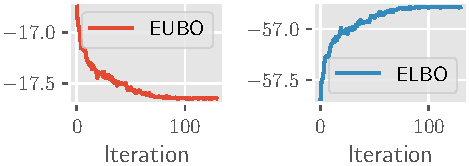
\includegraphics[height=0.17\textwidth]{img/train_eubo.pdf}
     &
     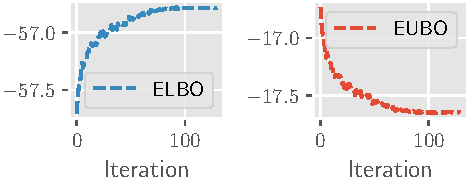
\includegraphics[height=0.17\textwidth]{img/train_elbo.pdf}\\
     (a) Unlearning from $\dr$ by minimizing EUBO
     & 
     (b) Retraining with $\dc$ by maximizing ELBO
\end{tabular}
\caption{Plots of EUBO and ELBO when (a) unlearning from $\dr$ and (b) retraining with $\dc$.}
\label{fig:eubovselbo}
\end{figure}
%
\subsection{Approximate Bayesian Unlearning with Approximate Posterior Belief
$q($\texorpdfstring{$\bm{\theta}$}{theta}$|\da)$}
\label{subsec:apprfull}
%
Often, in model training, only an approximate posterior belief\footnote{With a slight abuse of notation, we let  $q(\bm{\theta}|\da)$
be the approximate posterior belief that maximizes the ELBO $\mcl{L}$~\eqref{eq:elbo} (Sec.~\ref{sec:vi}) from Sec.~\ref{subsec:apprfull} onwards.} $q(\bm{\theta}|\da)$ (instead of the exact $p(\bm{\theta}|\da)$ in Sec.~\ref{subsec:exactfull}) of model parameters $\bm{\theta}$ given full data $\da$ can be learned, say, using 
%is available, which is different from the exact $p(\bm{\theta}|\da)$.
%We focus on the case that $q(\bm{\theta}|\da)$ is obtained from 
VI by maximizing the ELBO (Sec.~\ref{sec:vi}).
Our proposed unlearning methods are parsimonious in requiring only $q(\bm{\theta}|\da)$ and erased data $\dr$ to be available,
which makes unlearning even more challenging since there is no further 
% considers a parsimonious approach requiring only $q(\bm{\theta}|\da)$ and $\dr$ %(and $\bar{\dc}$ if $\dc$ and $\dr$ are not conditionally independent given $\bm{\theta}$)
%without any additional 
information about $p(\bm{\theta}|\da)$ nor the difference between $p(\bm{\theta}|\da)$ vs.~$q(\bm{\theta}|\da)$. 
%To perform unlearning, we need to mitigate the issue caused by the difference between the approximate $q(\bm{\theta}|\da)$ and the exact $p(\bm{\theta}|\da)$.
%which is elaborated in the next subsection.
%
%In this subsection, an approximate full-data posterior $q(\bm{\theta}|\da)$ is available, which is assumed to be obtained from VI (Sec.~\ref{sec:vi}). 
So, we estimate the unknown $p(\bm{\theta}|\dc)$~\eqref{eq:suffdata} with
%As the exact full-data posterior is unknown, we define the following probability, which is the counterpart of \eqref{eq:suffdata} given an approximate full-data posterior:
%
\begin{equation}
\tilde{p}(\bm{\theta}|\dc)\ \  \propto\ \ {q(\bm{\theta}|\da)}/{p(\dr| \bm{\theta})}
\label{eq:postapprx}
\end{equation}
%
%Since there is no additional information about the exact $p(\bm{\theta}|\da)$, we
and minimize the KL divergence between the approximate posterior belief recovered by directly unlearning from erased data $\dr$
%given remaining data $\dc$ 
vs.~$\tilde{p}(\bm{\theta}|\dc)$~\eqref{eq:postapprx} instead. We will discuss  two novel tricks below to alleviate the undesirable consequence of using $\tilde{p}(\bm{\theta}|\dc)$ instead of the unknown $p(\bm{\theta}|\dc)$~\eqref{eq:suffdata}.
%
\subsubsection{EUBO with Adjusted Likelihood}
\label{subsubsec:eubo}
%
Let the loss function $\text{KL}[\eubo(\bm{\theta}|\dc)\ \Vert\ \tilde{p}(\bm{\theta}|\dc)]$ be minimized w.r.t.~the approximate posterior belief $\eubo(\bm{\theta}|\dc)$ that is recovered by directly unlearning from erased data $\dr$. 
Similar to Proposition~\ref{theo:eubo}, $\eubo(\bm{\theta}|\dc)$ can be optimized by minimizing the following EUBO:
%
\begin{equation}
\widetilde{\mcl{U}} \triangleq \int \eubo(\bm{\theta}|\dc)\ \log p(\dr|\bm{\theta})\ \text{d}\bm{\theta} + \text{KL}[\eubo(\bm{\theta}|\dc)\ \Vert\ q(\bm{\theta}|\da)]
\label{eq:euboapprx}
\end{equation}
%
%It can be observed that $\widetilde{\mcl{U}}$~\eqref{eq:euboapprx} 
which follows from simply replacing the unknown $p(\bm{\theta}|\da)$ in $\mcl{U}$~\eqref{eq:eubo} with $q(\bm{\theta}|\da)$. 
%in Proposition~\ref{theo:eubo}. 
We discuss the difference between $p(\bm{\theta}|\da)$ vs.~$q(\bm{\theta}|\da)$ in the remark below:\vspace{1mm}
%
\begin{remark}
\label{rmk:inacc}
We analyze two possible sources of inaccuracy in $q(\bm{\theta}|\da)$ that is learned using VI by minimizing the loss function $\text{KL}[q(\bm{\theta}|\da)\ \Vert\ p(\bm{\theta}|\da)]$ (Sec.~\ref{sec:vi}).
%Since $q(\bm{\theta}|\da)$ is obtained using VI by minimizing $\text{KL}[q(\bm{\theta}|\da)\ \Vert\ p(\bm{\theta}|\da)]$, we focus on $2$ possible sources of inaccuracy between $q(\bm{\theta}|\da)$ and $p(\bm{\theta}|\da)$.
Firstly, $q(\bm{\theta}|\da)$ often underestimates the variance of $p(\bm{\theta}|\da)$: Though $q(\bm{\theta}|\da)$ tends to be close to $0$ at values of $\bm{\theta}$ where $p(\bm{\theta}|\da)$ is close to $0$, the reverse is not enforced \cite{bishop2006pattern} (see, for example, Fig.~\ref{fig:adjustedvi}).
So, $q(\bm{\theta}|\da)$ can differ from $p(\bm{\theta}|\da)$ at values of $\bm{\theta}$ where $q(\bm{\theta}|\da)$ is close to $0$.
Secondly, if $q(\bm{\theta}|\da)$ is learned through stochastic optimization of the ELBO (i.e., with stochastic samples of $\bm{\theta} \sim q(\bm{\theta}|\da)$ in each iteration of SGA), then it is unlikely that the ELBO is maximized using samples of $\bm{\theta}$ with small $q(\bm{\theta}|\da)$ (Fig.~\ref{fig:adjustedvi}). 
Thus, both sources of inaccuracy primarily occur at values of $\bm{\theta}$ with small $q(\bm{\theta}|\da)$. Though it can also be inaccurate at values of $\bm{\theta}$ with large $q(\bm{\theta}|\da)$, such an inaccuracy can be reduced by representing $q(\bm{\theta}|\da)$ with a complex distribution (Sec.~\ref{sec:vi}).
%with a complex approximate posterior belief.
\end{remark}
%
\begin{figure}
\centering
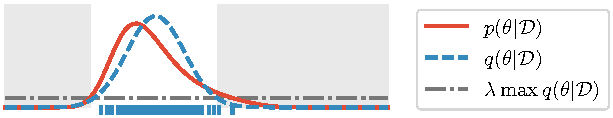
\includegraphics[width=0.63\textwidth]{img/vi_ep.pdf}
\caption{Plot of  $q(\bm{\theta}|\da)$ learned using VI. Gray shaded region corresponds to values of $\bm{\theta}$ where $q(\bm{\theta}|\da) \le \lambda \max_{\bm{\theta}'} q(\bm{\theta}'|\da)$. Vertical blue strips on  horizontal axis show $100$ samples of $\bm{\theta} \sim q(\bm{\theta}|\da)$.}
\label{fig:adjustedvi}
\end{figure}
%
Remark~\ref{rmk:inacc} motivates us to curb unlearning at values of $\bm{\theta}$ with small $q(\bm{\theta}|\da)$ by proposing our first novel trick of an adjusted likelihood of the erased data:
%, denoted as $p_{\text{adj}}(\dr|\bm{\theta})$, as follows:
%
\begin{equation}
p_{\text{adj}}(\dr|\bm{\theta}; \lambda) \triangleq 
	\begin{cases}
		p(\dr|\bm{\theta}) &\text{ if } q(\bm{\theta}|\da) > \lambda \max_{\bm{\theta}'} q(\bm{\theta}'|\da)\ ,\\
		1 &\text{ otherwise (i.e., shaded area in Fig.~\ref{fig:adjustedvi})}\ ;
		%&\text{ if } q(\bm{\theta}|\da) \le \lambda \max_{\bm{\theta}'} q(\bm{\theta}'|\da)
	\end{cases}
\label{eq:likelihoodadj}
\end{equation}
%
for any $\bm{\theta}$ where $\lambda \in [0,1]$ controls the magnitude of a threshold under which  $q(\bm{\theta}|\da)$ is considered small. To understand the effect of $\lambda$, let $\tilde{p}_{\text{adj}}(\bm{\theta}|\dc; \lambda) \propto q(\bm{\theta}|\da) / p_{\text{adj}}(\dr| \bm{\theta}; \lambda)$, i.e., by replacing $p(\dr| \bm{\theta})$ in \eqref{eq:postapprx} with $p_{\text{adj}}(\dr| \bm{\theta}; \lambda)$. Then, using~\eqref{eq:likelihoodadj},
%
\begin{equation}
\tilde{p}_{\text{adj}}(\bm{\theta}|\dc; \lambda) \propto 
	\begin{cases}
		q(\bm{\theta}|\da) / p(\dr| \bm{\theta}) &\text{ if } q(\bm{\theta}|\da) > \lambda \max_{\bm{\theta}'} q(\bm{\theta}'|\da)\ ,\\
		q(\bm{\theta}|\da) &\text{ otherwise (i.e., shaded area in Fig.~\ref{fig:adjustedvi})\ .}
		%&\text{ if } q(\bm{\theta}|\da) \le \lambda \max_{\bm{\theta}'} q(\bm{\theta}'|\da)
	\end{cases}
\label{eq:postappradj}
\end{equation}
%
According to~\eqref{eq:postappradj}, unlearning is therefore  focused at values of $\bm{\theta}$ with sufficiently large $q(\bm{\theta}|\da)$ (i.e.,
%Therefore, we would like to perform unlearning only where 
$q(\bm{\theta}|\da) > \lambda \max_{\bm{\theta}'} q(\bm{\theta}'|\da)$).
%(i.e., sufficiently large) as explained Remark~\ref{rmk:inacc}. 
Let the loss function $\text{KL}[\eubo(\bm{\theta}|\dc; \lambda)\ \Vert\ \tilde{p}_{\text{adj}}(\bm{\theta}|\dc; \lambda)]$ be minimized w.r.t.~the approximate posterior belief $\eubo(\bm{\theta}|\dc; \lambda)$ that is recovered by directly unlearning from erased data $\dr$.
Similar to~\eqref{eq:euboapprx},  %Proposition~\ref{theo:eubo}, 
$\eubo(\bm{\theta}|\dc; \lambda)$ can be optimized by minimizing the following EUBO:
%
\begin{equation}
\widetilde{\mcl{U}}_{\text{adj}}(\lambda) \triangleq \int \eubo(\bm{\theta}|\dc; \lambda)\ \log p_{\text{adj}}(\dr|\bm{\theta}; \lambda)\ \text{d}\bm{\theta} + \text{KL}[\eubo(\bm{\theta}|\dc; \lambda)\ \Vert\ q(\bm{\theta}|\da)]
\label{eq:euboapprxadj}
\end{equation}
%
which follows from replacing $p(\dr|\bm{\theta})$ in \eqref{eq:euboapprx} with $p_{\text{adj}}(\dr|\bm{\theta}; \lambda)$.
Note that $\eubo(\bm{\theta}|\dc; \lambda)$ can be represented by a simple distribution (e.g., Gaussian) or a complex one (e.g., generative neural network, IAF). 
%The objective $\widetilde{\mcl{U}}_{\text{adj}}(\lambda)$ in \eqref{eq:euboapprxadj} can also be optimized with stochastic optimization in a similar manner to optimizing ELBO in Sec.~\ref{sec:vi}. 
We initialize $\eubo(\bm{\theta}|\dc; \lambda)$ at $q(\bm{\theta}|\da)$ for achieving empirically faster convergence.
When $\lambda=0$, $\widetilde{\mcl{U}}_{\text{adj}}(\lambda=0)$ reduces to $\widetilde{\mcl{U}}$~\eqref{eq:euboapprx}, i.e., EUBO is minimized without the adjusted likelihood. As a result,  $\eubo(\bm{\theta}|\dc; \lambda=0)=\eubo(\bm{\theta}|\dc)$.
As $\lambda$ increases, unlearning is focused on a smaller and smaller region of $\bm{\theta}$ with sufficiently large $q(\bm{\theta}|\da)$.
When $\lambda$ reaches $1$, no unlearning is performed since 
%The value of $\lambda$ allows a trade-off between removing the effects of $\dr$ and maintaining the performance of the model (by being close to the full-data posterior belief $q(\bm{\theta}|\da)$). 
%For example, when $\lambda = 1$, no unlearning is performed. This is because
$\tilde{p}_{\text{adj}}(\bm{\theta}|\dc; \lambda=1) = q(\bm{\theta}|\da)$, which results in $\eubo(\bm{\theta}|\dc; \lambda=1) = q(\bm{\theta}|\da)$ minimizing the loss function $\text{KL}[\eubo(\bm{\theta}|\dc; \lambda=1)\ \Vert\ \tilde{p}_{\text{adj}}(\bm{\theta}|\dc; \lambda=1)]$.\vspace{1mm} 
%On the other hand, we use $\eubo(\bm{\theta}|\dc)$ to mean $\eubo(\bm{\theta}|\dc; \lambda=0)$. $\widetilde{\mcl{U}}_{\text{adj}}(\lambda=0)$ is equal to $\widetilde{\mcl{U}}$, so it is equivalent to directly minimizing EUBO without the adjusted likelihood.\vspace{1mm}
% The value of $\lambda$ can be tuned during the training of the model (i.e., training for $q(\bm{\theta}|\da)$), by comparing the marginal likelihood from $\eubo(\bm{\theta}|\dc; \lambda)$ with that from the re-trained posterior belief.
\todo{should we mention how to choose $\lambda$?}
%
\begin{example}
\label{exp:gamma}
% prior distribution: N(0,1)
% groundtruth: Gamma(shape=np.exp(1.0), rate=np.exp(1.0))
% unknown concentration (alpha, or shape)
% 20 data points, remove 5 data points (the smallest 5 data points)
% so unlearned posterior of shape should move to the right
% as mean of Gamma = alpha / beta (shape / rate)
To visualize the effect of varying $\lambda$ on $\eubo(\bm{\theta}|\dc;\lambda)$, we consider learning the shape $\alpha$ of a Gamma distribution with a known rate %$\beta=2.7$ 
(i.e., $\bm{\theta} = \alpha$): $\da$ are $20$ samples of the Gamma distribution, $\dr$ are the smallest $5$ samples in $\da$, and the (non-conjugate) prior belief and approximate %(unlearned, re-trained, and full-data) 
posterior beliefs of $\alpha$ are all Gaussians.
Fig.~\ref{fig:expunlearn}a shows the approximate posterior beliefs  $\eubo(\bm{\theta}|\dc; \lambda)$ with varying $\lambda$ as well as  $q(\bm{\theta}|\da)$ and 
%the approximate re-trained posterior belief
$q(\bm{\theta}|\dc)$ learned using VI. 
As explained above, $\eubo(\bm{\theta}|\dc, \lambda=1) = q(\bm{\theta}|\da)$. 
When $\lambda = 0.001$, $\eubo(\bm{\theta}|\dc, \lambda=0.001)$ is close to %the approximate re-trained posterior belief
$q(\bm{\theta}|\dc)$. 
However, as $\lambda$ decreases to $0$, $\eubo(\bm{\theta}|\dc, \lambda)$ moves away from $q(\bm{\theta}|\dc)$.
%, which is potentially due to the underestimation of the variance of EUBO. 
\end{example}
%
% \begin{figure}[ht]
% \centering
% \begin{tabular}{c}
% 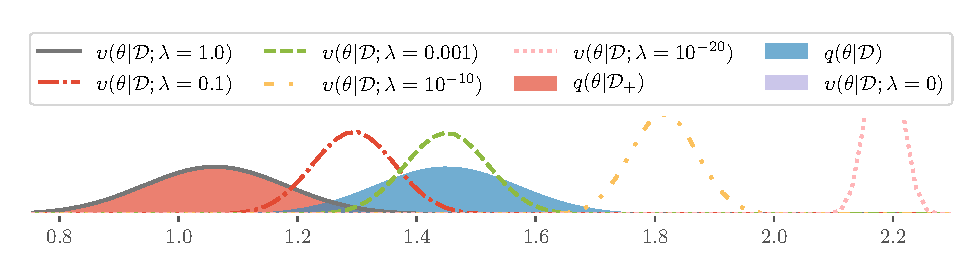
\includegraphics[trim={4mm 4mm 0mm 5mm}, clip, height=0.2\textwidth]{img/gamma_unknown_mean/eubo_unlearn.pdf}
% \\
% 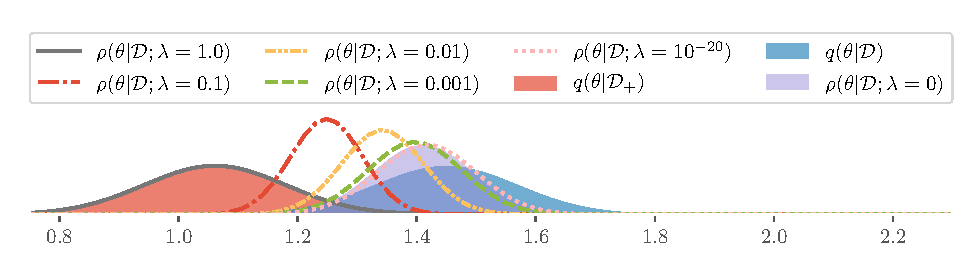
\includegraphics[trim={4mm 4mm 0mm 5mm}, clip, height=0.2\textwidth]{img/gamma_unknown_mean/elbo_unlearn.pdf}
% \end{tabular}
% \caption{Plot of approximate unlearned posterior beliefs obtained by minimizing EUBO (top plot), and reverse KL (bottom plot) (vertical axis is probability density; horizontal axis is $\theta = \alpha$).}
% \label{fig:expunlearn}
% \end{figure}
%
\begin{figure}
\centering
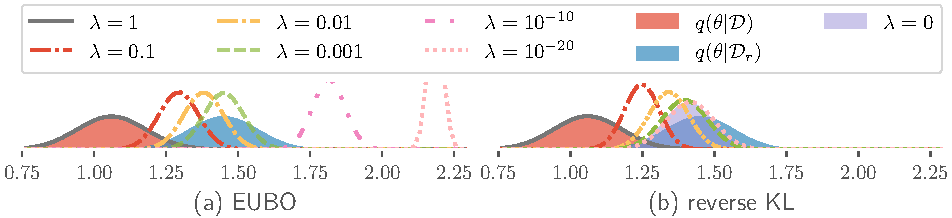
\includegraphics[width=\textwidth]{img/gamma_unknown_mean/gamma_unlearn.pdf}
\caption{Plot of approximate posterior beliefs with varying $\lambda$ obtained by minimizing (a) EUBO (i.e., $\eubo(\bm{\theta}|\dc;\lambda)$) and (b) reverse KL (i.e., $\elbo(\bm{\theta}|\dc;\lambda)$); horizontal axis denotes $\theta = \alpha$.
In (a), a huge probability
%the majority of the
mass of $\eubo(\bm{\theta}|\dc, \lambda=0)$ is at large values of $\alpha$ beyond the plotting area and the top of the plot of $\eubo(\bm{\theta}|\dc, \lambda=10^{-20})$ is cut off due to lack of space.
}
\label{fig:expunlearn}
\end{figure}
\todo{need details about this example}
%
%Minimizing $\text{KL}[\eubo(\bm{\theta}|\dc; \lambda)\ \Vert\ \tilde{p}_{\text{adj}}(\bm{\theta}|\dc; \lambda)]$ 
The optimized $\eubo(\bm{\theta}|\dc; \lambda)$
suffers from the same issue of underestimating the variance as $q(\bm{\theta}|\da)$ learned using VI (see Remark~\ref{rmk:inacc}), 
especially when $\lambda$ tends to $0$ (e.g., see $\eubo(\bm{\theta}|\dc; \lambda=10^{-20})$ in Fig.~\ref{fig:expunlearn}a).
%In other words, by first learning the approximate full-data posterior belief $q(\bm{\theta}|\da)$ with VI, then unlearning $\dr$ from $q(\bm{\theta}|\da)$ to obtain $\eubo(\bm{\theta}|\dc)$, underestimating the variance can happen twice if $\lambda$ is too small.
%(i.e., $p(\bm{\theta}|\dc) > \tilde{p}_{\text{adj}}(\bm{\theta}|\dc; \lambda) > \eubo(\bm{\theta}|\dc; \lambda)$ where $\tilde{p}(\bm{\theta}|\dc)$ is close to $0$ and $\lambda$ is close to $0$).
%This can lead to undesired $\eubo(\bm{\theta}|\dc; \lambda)$ (e.g., $\eubo(\bm{\theta}|\dc; \lambda=10^{-20})$ in Fig.~\ref{fig:expunlearn}a).
Though this issue can be mitigated by tuning $\lambda$ in the adjusted likelihood~\eqref{eq:likelihoodadj}, we may not want to risk facing the consequence of picking a value of $\lambda$ that is too small.
So, in Sec.~\ref{subsubsec:rkl}, we will propose another novel trick that is not inconvenienced by this issue.
%In the next section, we explore an unlearning method that does not suffer from this issue.
%
\subsubsection{Reverse KL}
\label{subsubsec:rkl}
%
%To avoid the issue of underestimating the variance of $\tilde{p}(\bm{\theta}|\dc)$ in EUBO, 
Let the loss function be the reverse KL divergence $\text{KL}[\tilde{p}(\bm{\theta}|\dc)\ \Vert\ \elbo(\bm{\theta}|\dc)]$ that is minimized w.r.t.~the approximate posterior belief $\elbo(\bm{\theta}|\dc)$ recovered by directly unlearning from erased data $\dr$. 
In contrast to the optimized $\eubo(\bm{\theta}|\dc; \lambda)$
from minimizing EUBO~\eqref{eq:euboapprxadj}, 
the optimized $\elbo(\bm{\theta}|\dc)$ from minimizing the reverse KL divergence 
overestimates (instead of underestimates) the variance of $\tilde{p}(\bm{\theta}|\dc)$ \cite{bishop2006pattern}: If $\tilde{p}(\bm{\theta}|\dc)$ is close to $0$, then $\elbo(\bm{\theta}|\dc)$ is not necessarily close to $0$.
%Hence, it avoids underestimating the variance of $\tilde{p}(\bm{\theta}|\dc)$ in minimizing EUBO.
From~\eqref{eq:postapprx}, the reverse KL divergence can be expressed as follows:
%
\begin{equation}
\text{KL}[\tilde{p}(\bm{\theta}|\dc)\ \Vert\ \elbo(\bm{\theta}|\dc)] 
	= C_0 - C_1\  \mbb{E}_{q(\bm{\theta}|\da)} \left[(\log \elbo(\bm{\theta}|\dc))/{p(\dr|\bm{\theta})}  \right]
\label{eq:reversekl}
\end{equation}
%
where $C_0$ and $C_1$ are constants independent of $\elbo(\bm{\theta}|\dc)$. So, the reverse KL divergence~\eqref{eq:reversekl} can be minimized by maximizing $\mbb{E}_{q(\bm{\theta}|\da)} [ (\log \elbo(\bm{\theta}|\dc)) / p(\dr|\bm{\theta}) ]$ with \emph{stochastic gradient ascent} (SGA).
We also initialize $\elbo(\bm{\theta}|\dc)$ at $q(\bm{\theta}|\da)$ for achieving empirically faster convergence.
Since stochastic optimization is performed with samples of $\bm{\theta} \sim q(\bm{\theta}|\da)$ in each iteration of SGA, it is unlikely that the reverse KL divergence~\eqref{eq:reversekl} is minimized using samples of $\bm{\theta}$ with small $q(\bm{\theta}|\da)$.
This naturally curbs unlearning at values of $\bm{\theta}$ with small $q(\bm{\theta}|\da)$, as motivated by Remark~\ref{rmk:inacc}.
%
%As $p(\dr|\bm{\theta}, \bar{\dc})$ can be small for some values of $\bm{\theta}$, which makes $\mbb{E}_{q(\bm{\theta}|\da)} \left[ \left(\log \elbo(\bm{\theta}|\dc)\right) / p(\dr|\bm{\theta}, \bar{\dc}) \right]$ large, we maximize $C_1 \mbb{E}_{q(\bm{\theta}|\da)} \left[ \left(\log \elbo(\bm{\theta}|\dc)\right) / p(\dr|\bm{\theta}, \bar{\dc}) \right]$, where $C_1 = 1 / \mbb{E}_{q(\bm{\theta}|\da)} \left[ 1 / p(\dr|\bm{\theta}, \bar{\dc}) \right]$ estimated over a number of samples of $\bm{\theta} \sim q(\bm{\theta}|\da)$. 
%
% Although the first source of inaccuracy in Remark~\ref{rmk:inacc} (i.e., underestimating the variance) is mitigated, the inaccuracy can still happen from the second source of inaccuracy. Fortunately, since $C_1 \mbb{E}_{q(\bm{\theta}|\da)} \left[ \left(\log \elbo(\bm{\theta}|\dc)\right) / p(\dr|\bm{\theta}, \bar{\dc}) \right]$ is maximized with stochastic optimization (i.e., at each optimization iteration, random samples $\bm{\theta} \sim q(\bm{\theta}|\da)$ are drawn to estimate the expectation), the probability of drawing a sample $\bm{\theta}$ with small $q(\bm{\theta}|\da)$ is low. This naturally handles the second source of inaccuracy. 
%
On the other hand, it is still possible to employ the same trick of adjusted likelihood (Sec.~\ref{subsubsec:eubo}) by minimizing the reverse KL divergence  $\text{KL}[\tilde{p}_{\text{adj}}(\bm{\theta}|\dc; \lambda)\ \Vert\ \elbo(\bm{\theta}|\dc; \lambda)]$ as the loss function or, equivalently,  maximizing 
$\mbb{E}_{q(\bm{\theta}|\da)} [(\log \elbo(\bm{\theta}|\dc; \lambda))/p_{\text{adj}}(\dr|\bm{\theta}; \lambda) ]$
%
%constructing a new objective:
%. In other words, using the adjusted likelihood $p_{\text{adj}}(\dr|\bm{\theta}, \bar{\dc}; \lambda)$ in \eqref{eq:likelihoodadj}, we have a new objective function:
%
%\begin{equation}
%\[
%\widetilde{\mcl{L}}_{\text{adj}}(\lambda) = \mbb{E}_{q(\bm{\theta}|\da)} \left[(\log \elbo(\bm{\theta}|\dc; \lambda))/p_{\text{adj}}(\dr|\bm{\theta}; \lambda)  \right]
%\]
%\label{eq:reversekladj}
%\end{equation}
%
%maximizing of which is equivalent to minimizing $\text{KL}[\tilde{p}_{\text{adj}}(\bm{\theta}|\dc; \lambda)\ \Vert\ \elbo(\bm{\theta}|\dc; \lambda)]$ 
where $p_{\text{adj}}(\dr|\bm{\theta}; \lambda)$ and $\tilde{p}_{\text{adj}}(\bm{\theta}|\dc; \lambda)$ are previously defined in \eqref{eq:likelihoodadj} and \eqref{eq:postappradj}, respectively.
The role of $\lambda$ here is the same as that in \eqref{eq:euboapprxadj}. 
%For example, when $\lambda = 1$, no unlearning is performed (since $\tilde{p}_{\text{adj}}(\bm{\theta}|\dc; \lambda=1) = q(\bm{\theta}|\da)$). On the other hand, when $\lambda = 0$, the objective function\eqref{eq:reversekladj} is the same as the second term in \eqref{eq:reversekl} (i.e., $\tilde{p}_{\text{adj}}(\bm{\theta}|\dc; \lambda=0) = \tilde{p}(\bm{\theta}|\dc)$).

To illustrate the difference between minimizing the reverse KL divergence~\eqref{eq:reversekl} and EUBO~\eqref{eq:euboapprxadj}, Fig.~\ref{fig:expunlearn}b shows the approximate  posterior beliefs $\elbo(\bm{\theta}|\dc; \lambda)$ with varying $\lambda$. It can be observed that $\elbo(\bm{\theta}|\dc; \lambda=1) = q(\bm{\theta}|\da)$ (i.e., no unlearning). In contrast to minimizing EUBO (Fig.~\ref{fig:expunlearn}a), as $\lambda$ decreases to $0$, $\elbo(\bm{\theta}|\dc; \lambda)$ does not deviate  that much from  $q(\bm{\theta}|\dc)$, even when $\lambda = 0$ (i.e.,  the reverse KL divergence is minimized without the adjusted likelihood). 
%As explained above, by minimizing the reverse KL distance with stochastic gradient descent,
This is because
the optimized $\elbo(\bm{\theta}|\dc; \lambda)$ is naturally more protected from both sources of inaccuracy (Remark~\ref{rmk:inacc}), as explained above.
Hence, we do not have to be as concerned about picking a small value of $\lambda$, which is also consistently observed in our experiments  (Sec.~\ref{sec:experiment}).
%is because the our approach of minimizing the reverse KL  can mitigate both sources of inaccuracy as explained above.
%
\section{Experiments and Discussion}
\label{sec:experiment}
%
This section empirically demonstrates our unlearning methods on Bayesian models such as sparse Gaussian process and logistic regression using synthetic and real-world datasets.
Further experimental results on Bayesian linear regression and with a bimodal posterior belief are reported in Appendices~\ref{app:lr} and~\ref{app:multimode}, respectively.
In our experiments, each dataset comprises pairs of input $\mbf{x}$ and its corresponding output/observation $y_{\mbf{x}}$.
We use RMSProp as the SGA algorithm with a learning rate of $10^{-4}$.
To assess the performance of our unlearning methods (i.e., by directly unlearning from erased data $\dr$),
we consider the difference between their induced predictive distributions vs.~that obtained using VI from retraining with remaining data $\dc$,
as motivated from Sec.~\ref{subsec:exactfull}.
To do this, we use a {\bf performance metric} that measures the KL divergence between the approximate predictive distributions
\[
\eubo(y_{\mbf{x}}|\dc) \triangleq \int p(y_{\mbf{x}}|\bm{\theta})\  \eubo(\bm{\theta}|\dc;\lambda)\ \text{d}\bm{\theta}
\quad\text{or}\quad
\elbo(y_{\mbf{x}}|\dc) \triangleq \int 
p(y_{\mbf{x}}|\bm{\theta})\ \elbo(\bm{\theta}|\dc;\lambda)\ \text{d}\bm{\theta}
\]
vs.~$q(y_{\mbf{x}}|\dc) \triangleq \int  p(y_{\mbf{x}}|\bm{\theta})\ q(\bm{\theta}|\dc)\  \text{d}\bm{\theta}$ where 
$\eubo(\bm{\theta}|\dc; \lambda)$ and $\elbo(\bm{\theta}|\dc; \lambda)$
are optimized
by, respectively, minimizing  EUBO~\eqref{eq:euboapprxadj} and \emph{reverse KL} (rKL) divergence~\eqref{eq:reversekl} while requiring only $q(\bm{\theta}|\da)$ and erased data $\dr$ (Sec.~\ref{subsec:apprfull}), and $q(\bm{\theta}|\dc)$ is learned using VI (Sec.~\ref{sec:vi}).
%obtained by marginalizing over the unlearned posterior belief (using EUBO, $\eubo(y_{\mbf{x}}|\dc) \triangleq \int \eubo(\bm{\theta}|\dc;\lambda)\ p(y_{\mbf{x}}|\bm{\theta})\ \text{d}\bm{\theta}$, or reverse KL, $\elbo(y_{\mbf{x}}|\dc) \triangleq \int \elbo(\bm{\theta}|\dc;\lambda)\ p(y_{\mbf{x}}|\bm{\theta})\ \text{d}\bm{\theta}$) and that obtained by marginalizing over the approximate retrained posterior belief (using VI), $q(y_{\mbf{x}}|\dc) \triangleq \int q(\bm{\theta}|\dc) p(y_{\mbf{x}}|\bm{\theta})\ \text{d}\bm{\theta}$.
The above predictive distributions are computed via sampling with $100$ samples of $\bm{\theta}$.
For tractability reasons,
we evaluate the above performance metric over  finite input domains, specifically, over that in $\dr$ and $\dc$, which allows us to assess the 
%Since it is intractable to compute the above performance metric over the entire (possibly continuous) input domain, we restrict the it to $\dc$ and $\dr$ separately. 
%The intuition is to quantify the 
performance of our unlearning methods on both the erased and remaining data, i.e., whether they can fully unlearn from $\dr$ yet not forget nor catastrophically unlearn from $\dc$, respectively.
For example, the performance of our EUBO-based unlearning method over $\dr$ is shown as an average (with standard deviation) of the KL divergences between $\eubo(y_{\mbf{x}}|\dc)$ vs.~$q(y_{\mbf{x}}|\dc)$ over all $(\mbf{x},y_{\mbf{x}}) \in \dr$.
% $\mcl{E}_{\eubo} (\dr; \lambda)$:
% %
% \begin{equation*}
% \textstyle
% \mcl{E}_{\eubo} (\dr; \lambda) \triangleq \sqrt{ |\dr|^{-1} \sum_{y_{\mbf{x}} \in \dr} \left( 
%     q_{\eubo}(y_{\mbf{x}}|\dc) - q(y_{\mbf{x}}|\dc)
% \right)^2}\ .
% \end{equation*}
%
%As unlearning aims to recover the unlearned posterior belief from $q(\bm{\theta}|\da)$. 
We also plot an average (with standard deviation) of the KL divergences between $q(y_{\mbf{x}}|\da)$ vs.~$q(y_{\mbf{x}}|\dc)$ over $\dc$ and $\dr$ as \emph{baselines} (i.e., representing no unlearning), which is expected to be larger than that of our unlearning methods (i.e., if performing well)
and labeled as \emph{full} in the plots below.
%The desirable values of the KL distance between $\eubo(y_{\mbf{x}}|\dc)$ (or $\elbo(y_{\mbf{x}}|\dc)$) are those smaller than the baseline.
% a desirable value of RMS of an unlearning approach should be smaller than the RMS of $q(\bm{\theta}|\da)$, denoted as $\mcl{E}_{\text{full}} (\dc)$ and $\mcl{E}_{\text{full}} (\dr)$. For example, $\mcl{E}_{\eubo} (\dr; \lambda) < \mcl{E}_{\text{full}} (\dr)$ is desirable for EUBO.
% Thus, we compute the RMS of $q(\bm{\theta}|\da)$ on $\dc$ and $\dr$ as baselines, which are labeled as \emph{full} in plots. 
%In all experiments, the data are conditionally independent given the model parameters, so $\bar{\dc} = \emptyset$.
%
% As the approximate re-trained posterior belief $q(\bm{\theta}|\dc)$ may be different from the exact re-trained posterior belief $p(\bm{\theta}|\dc)$, and it is difficult to obtain $p(\bm{\theta}|\dc)$ in the following experiments, we compare the log of the marginal likelihood from the approximate re-trained posterior belief $q(\bm{\theta}|\dc)$ and that from the approximate unlearned posterior belief ($\eubo(\bm{\theta}|\dc)$ trained with EUBO, and $\elbo(\bm{\theta}|\dc)$ trained with \emph{reverse KL} (rKL)). Thus, the performance measure is the \emph{mean absolute error} (MAE) of the log of the marginal likelihood, computed over the removed dataset $\dr$ and the remaining dataset $\dc$. For example, the performance measure of the EUBO approach on $\dc$ is denoted as $\text{MAE}_{q(\bm{\theta}|\dc)} (\dc; \eubo(\bm{\theta}|\dc; \lambda)) \triangleq |\dc|^{-1} \sum_{\mbf{y} \in \dc} |\mbb{E}_{\eubo(\bm{\theta}|\dc; \lambda)} \log p(\mbf{y}|\bm{\theta})
% - \mbb{E}_{q(\bm{\theta}'|\dc)} \log p(\mbf{y}|\bm{\theta}')|$ where $\mbf{y}$ is the observation of the model (similar definitions for $\text{MAE}_{q(\bm{\theta}|\dc)} (\dr; \eubo(\bm{\theta}|\dc; \lambda))$, $\text{MAE}_{q(\bm{\theta}|\dc)} (\dc; \elbo(\bm{\theta}|\dc; \lambda))$, and $\text{MAE}_{q(\bm{\theta}|\dc)} (\dr; \elbo(\bm{\theta}|\dc; \lambda))$). We also plot the MAE of the log of the marginal likelihood from the approximate full-data posterior belief compared with that from the approximate re-trained posterior belief as the baseline, i.e., MAE when no unlearning is performed. It is denoted as $\text{MAE}_{q(\bm{\theta}|\dc)} (\dc; q(\bm{\theta}|\da))$, $\text{MAE}_{q(\bm{\theta}|\dc)} (\dr; q(\bm{\theta}|\da))$ and labeled as \emph{full} in plots. 
% The intuition is that if an unlearning approach can achieve MAE less than $\text{MAE}_{q(\bm{\theta}|\dc)} (\dc; q(\bm{\theta}|\da))$ ($\text{MAE}_{q(\bm{\theta}|\dc)} (\dr; q(\bm{\theta}|\da))$), it is able to unlearn such that the marginal likelihood on the remaining (removed) dataset is closer to that from the approximate re-trained posterior belief than that from the approximate full-data posterior belief.
% The data are conditionally independent given the model parameters in the following experiments, so $\bar{\dc} = \emptyset$.
%
\todo{change the notation of MAE}
%
\subsection{Sparse Gaussian Process (GP) Classification with Synthetic Moon Dataset}
\label{subsec:expmoon}
%
This experiment is about unlearning a binary classifier that is previously trained with the synthetic moon dataset (Fig.~\ref{fig:moon}a). 
%shows the erased data $\dr$ (crosses) and the remaining data $\dc$ (dots).
The probability of input $\mbf{x} \in \mbb{R}^2$ being in the `blue' class (i.e., $y_{\mbf{x}} = 1$ and denoted by blue dots in Fig.~\ref{fig:moon}a) is defined as $1/(1 + \exp(f_{\mbf{x}}))$ where $f_{\mbf{x}}$ is a latent function modeled by a sparse GP \cite{quinonero2005unifying}, which is elaborated in Appendix~\ref{app:moon}. 
The parameters $\bm{\theta}$ of the sparse GP consist of $20$ inducing variables;
%The full-data (retrained and unlearned) 
 the approximate
posterior beliefs of $\bm{\theta}$ are thus 
%modeled with 
multivariate Gaussians (with full covariance matrices), as shown in Appendix~\ref{app:moon}.
By comparing Figs.~\ref{fig:moon}b and~\ref{fig:moon}c, it can be observed that after erasing $\dr$ (i.e., mainly in `yellow' class), $q(y_{\mbf{x}} = 1|\dc)$ increases at $\mbf{x} \in \dr$.
% The predictive distribution can be visualized using the mean $\mu_{\mbf{x}}$~\eqref{eq:gppostmean} of the GP posterior belief (Appendix~\ref{app:moon}) because $\mu_{\mbf{x}} < 0$ implies that $\mbf{x}$ is likely to be in the `blue' class; plots of both the mean and variance of the GP posterior belief are shown in Appendix~\ref{app:moon}.
% It can be observed by comparing Figs.~\ref{fig:moon}b and~\ref{fig:moon}c that after erasing $\dr$ (i.e., mainly in the `yellow' class), $\mu_{\mbf{x}}$ at each input $\mbf{x}$ in $\dr$ decreases, hence reducing the probability of the erased data in the `yellow' class.
%
% The mean of GP posterior of the latent function, denoted as $\mu_{\mbf{x}}$, given the approximate full-data posterior belief $q(\bm{\theta}|\da)$ and approximate re-trained posterior belief $q(\bm{\theta}|\dc)$ (trained with VI) are shown in Fig.~\ref{fig:moon}b,c.
% After removing $\dr$ (mainly in the ``yellow'' class), $\mu_{\mbf{x}}$ at the removed $\mbf{x}$ reduces, i.e., the probability of these $\mbf{x}$ in the ``yellow'' class reduces.
%
% \begin{figure}[ht]
% \centering
% \begin{tabular}{ccc}
% 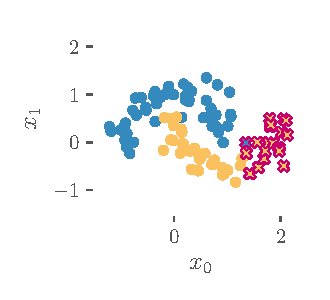
\includegraphics[trim={7mm 8mm 3mm 3mm}, clip,height=0.15\textwidth]{img/moon/moon_data.pdf}
% &
% 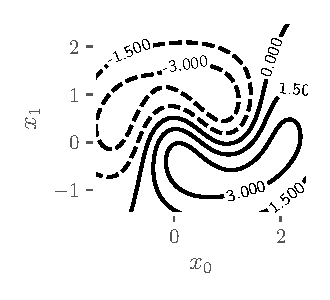
\includegraphics[trim={7mm 8mm 3mm 3mm}, clip,height=0.15\textwidth]{img/moon/moon_full_meanf.pdf}
% &
% 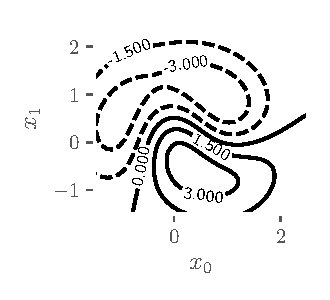
\includegraphics[trim={7mm 8mm 3mm 3mm}, clip,height=0.15\textwidth]{img/moon/moon_remain_meanf.pdf}
% \\
% (a) Moon dataset.
% &
% (b) $\mu_{\mbf{x}}$ given $q(\bm{\theta}|\da)$.
% &
% (c) $\mu_{\mbf{x}}$ given $q(\bm{\theta}|\dc)$.
% \end{tabular}
% \caption{Classification with moon dataset.}
% \label{fig:moon}
% \end{figure}
%
Figs.~\ref{fig:moon}d~and~\ref{fig:moon}e show results of the performance of our EUBO- and rKL-based unlearning methods over $\dc$ and $\dr$ with varying $\lambda$, respectively.\footnote{\label{log}Note that the log plots can only properly display the upper confidence interval of $1$ standard deviation (shaded area) and hence do not show the lower confidence interval.
%The shaded area does not include the area from the average to the average subtracted by the standard deviation (of the KL distance) which is not suitable for $\log$ plots due to its negative values.
}
When $\lambda = 10^{-9}$, EUBO performs reasonably well (compare Figs.~\ref{fig:moon}g~vs.~\ref{fig:moon}c) as its averaged KL divergence is smaller than that of $q(\bm{\theta}|\da)$ (i.e., baseline labeled as \emph{full}).
When $\lambda = 0$, EUBO performs poorly (compare Figs.~\ref{fig:moon}h~vs.~\ref{fig:moon}c) as its averaged KL divergence is much larger than that of $q(\bm{\theta}|\da)$, as shown in Figs.~\ref{fig:moon}d and~\ref{fig:moon}e.
%KL distances of EUBO increase significantly (larger than that of $q(\bm{\theta}|\da)$ in Figs.~\ref{fig:moon}d,e), which indicates its poor performance. 
This agrees with our discussion of the issue with picking too small a value of $\lambda$ for EUBO at the end of Sec.~\ref{subsubsec:eubo}.
In particular, catastrophic unlearning is observed as the input region containing $\dr$ (i.e., mainly in `yellow' class) has a high probability in `blue' class after unlearning in Fig.~\ref{fig:moon}h. 
On the other hand, when $\lambda = 0$, 
rKL performs well (compare Figs.~\ref{fig:moon}k~vs.~\ref{fig:moon}c) as its
KL divergence is much smaller than that of $q(\bm{\theta}|\da)$, as seen in  Figs.~\ref{fig:moon}d and~\ref{fig:moon}e. This agrees with our discussion at the end of Sec.~\ref{subsubsec:rkl} that rKL can work well without needing the adjusted likelihood. 

One may question how the performance of our unlearning methods would vary when erasing a large quantity of data or with different distributions of erased data (e.g., erasing the data randomly vs.~deliberately erasing all data in a given class). 
To address this question, 
we have discovered that a key factor influencing their unlearning performance in these scenarios is the difference between the posterior beliefs of model parameters $\bm{\theta}$ given remaining data $\dc$ vs.~that given full data $\da$, especially at values of $\bm{\theta}$ with small $q(\bm{\theta}|\da)$ since unlearning in such a region is curbed by the adjusted likelihood and reverse KL.
%
In practice, we expect such a difference not to be large due to the small quantity of erased data and redundancy in real-world datasets.
%
% In practice, we expect that the posterior belief of the model parameters given the remaining data does not differ much from that given the full data due to the small amount of erased data and the redundancy of information in the training data.
%
We will present the details of this study in Appendix~\ref{app:information} due to lack of space by considering how much $\dr$ reduces the entropy of $\bm{\theta}$ given $\dc$.
%using the notion of information gain on $\bm{\theta}$ from $\dr$ given $\dc$ 
%In fact, the answer can be elaborated with the notion of the information about 
%We also perform unlearning in a linear regression problem in Appendix~\ref{app:lr}.
%
% \begin{figure}[ht]
% \centering
% \begin{tabular}{@{}c@{}c@{}c@{}c@{}}
% \includegraphics[trim={3mm 3mm 3mm 3mm}, clip,height=0.15\textwidth]{img/likelihood_diff/moon_gauss_fullcov_likelihood_remain_retrain_f_legend.pdf}
% &
% 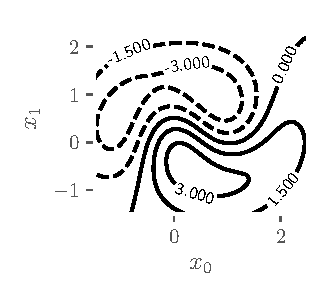
\includegraphics[trim={7mm 8mm 3mm 3mm}, clip,height=0.15\textwidth]{img/moon/moon_elbo_meanf_1e-05.pdf}
% &
% 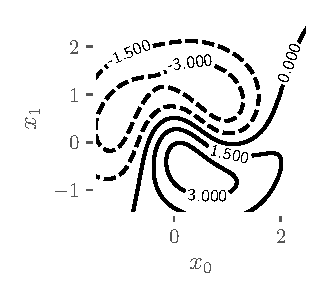
\includegraphics[trim={7mm 8mm 3mm 3mm}, clip,height=0.15\textwidth]{img/moon/moon_elbo_meanf_1e-09.pdf}
% &
% 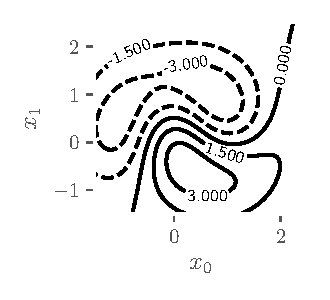
\includegraphics[trim={7mm 8mm 3mm 3mm}, clip,height=0.15\textwidth]{img/moon/moon_elbo_meanf_0_0.pdf}
% \\
% (a) $\dc$
% &
% (b)
% &
% (c)
% &
% (d)
% \\
% 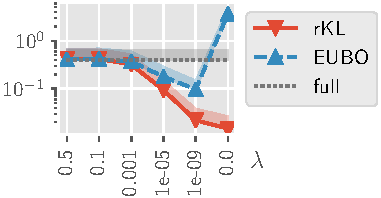
\includegraphics[trim={3mm 3mm 3mm 3mm}, clip,height=0.15\textwidth]{img/likelihood_diff/moon_gauss_fullcov_likelihood_remove_retrain_f_legend.pdf}
% &
% 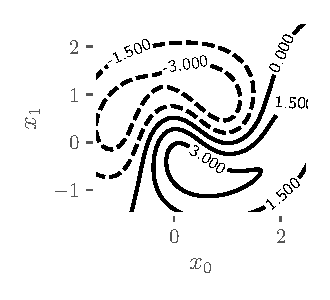
\includegraphics[trim={7mm 8mm 3mm 3mm}, clip,height=0.15\textwidth]{img/moon/moon_eubo_meanf_1e-05.pdf}
% &
% 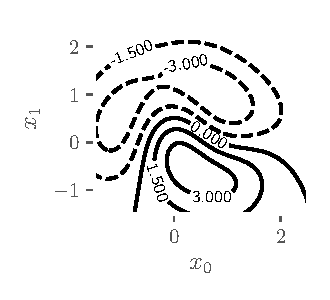
\includegraphics[trim={7mm 8mm 3mm 3mm}, clip,height=0.15\textwidth]{img/moon/moon_eubo_meanf_1e-09.pdf}
% &
% 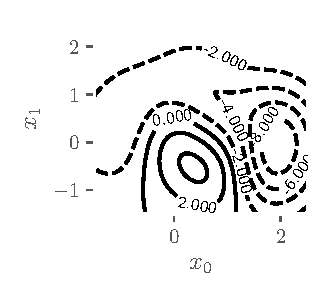
\includegraphics[trim={7mm 8mm 3mm 3mm}, clip,height=0.15\textwidth]{img/moon/moon_eubo_meanf_0_0.pdf}
% \\
% (e) $\dr$
% &
% (f)
% &
% (g)
% &
% (h)
% \end{tabular}
% \caption{ The difference in the marginal likelihoods of $\dc$ (a) and $\dr$ (e) trained with reverse KL (rKL) and EUBO and different values of $\lambda$. Plots of $\mu_{\mbf{x}}$ trained with rKL (b,c,d) and EUBO (f,g,h) where $\lambda = 10^{-5}$ (b,f), $10^{-9}$ (c,g), and $0$ (d,h). }
% \label{fig:moonresult}
% \end{figure}
%
\begin{figure}
\hspace{-2mm}
%\centering
\begin{tabular}{@{}c@{}}
    \begin{tabular}{@{}c@{}c@{}c@{}c@{}c@{}}
    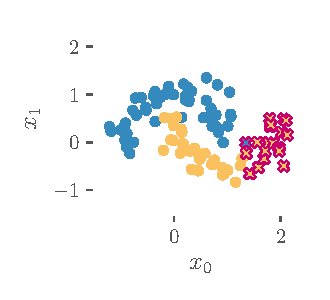
\includegraphics[trim={7mm 8mm 3mm 3mm}, clip,height=0.16\textwidth]{img/moon/moon_data.pdf}
    &
    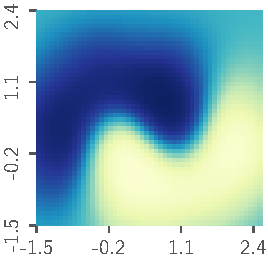
\includegraphics[height=0.15\textwidth]{img/moon/moon_full_prob.pdf}
    &
    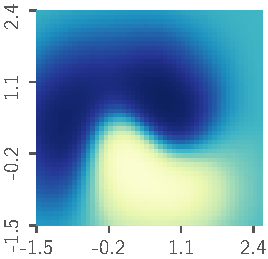
\includegraphics[height=0.15\textwidth]{img/moon/moon_remain_prob.pdf}
    & \hspace{-2mm}
    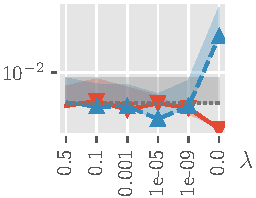
\includegraphics[height=0.15\textwidth]{img/likelihood_diff/moon_gauss_fullcov_likelihood_remain_retrain_f.pdf}
    &
    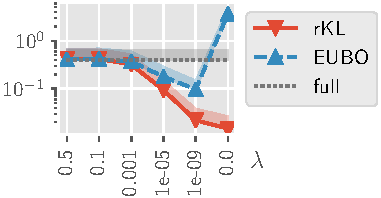
\includegraphics[height=0.15\textwidth]{img/likelihood_diff/moon_gauss_fullcov_likelihood_remove_retrain_f_legend.pdf}
    \\
    (a) Dataset
    &
    (b) $q(y_{\mbf{x}}=1| \da)$ % Train with $\da$
    & \hspace{1mm}
    (c) $q(y_{\mbf{x}}=1| \dc)$ % Retrain with $\dc$
    &
    (d) $\dc$
    &
    (e) $\dr$
    \end{tabular}
\vspace{2mm}\\
    \begin{tabular}{@{}c@{}c@{}c@{}|@{}c@{}c@{}c@{}}
    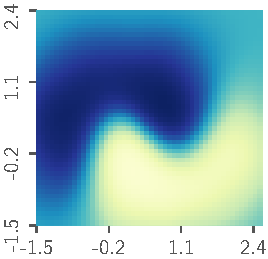
\includegraphics[height=0.135\textwidth]{img/moon/moon_eubo_prob_1e-05.pdf}
    &\hspace{2.5mm}
    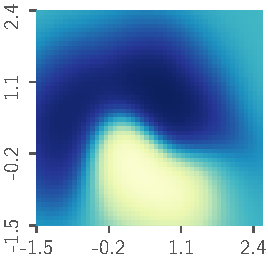
\includegraphics[height=0.135\textwidth]{img/moon/moon_eubo_prob_1e-09.pdf}
    &\hspace{2.5mm}
    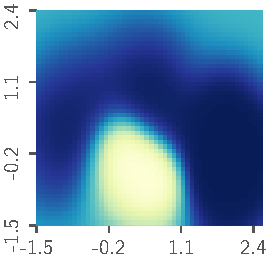
\includegraphics[height=0.135\textwidth]{img/moon/moon_eubo_prob_0_0.pdf}\hspace{2mm}
    &
    \hspace{2mm}
    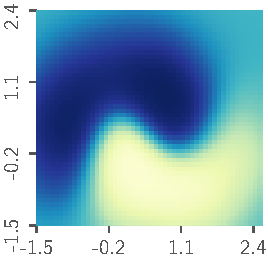
\includegraphics[height=0.135\textwidth]{img/moon/moon_elbo_prob_1e-05.pdf}
    &\hspace{2.5mm}
    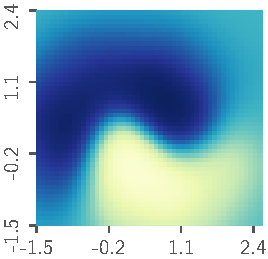
\includegraphics[height=0.135\textwidth]{img/moon/moon_elbo_prob_1e-09.pdf}
    &\hspace{2.5mm}
    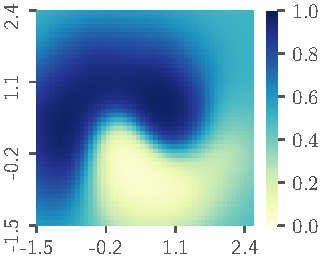
\includegraphics[height=0.135\textwidth]{img/moon/moon_elbo_prob_0_0.pdf}
    \\
    (f) $\lambda = 10^{-5}$
    &
    (g) $\lambda = 10^{-9}$
    &
    (h) $\lambda = 0$
    &
    (i) $\lambda = 10^{-5}$
    &
    (j) $\lambda = 10^{-9}$
    &
    (k) $\lambda = 0$
    \end{tabular}
\end{tabular}\vspace{-0.7mm}
\caption{Plots of (a) synthetic moon dataset with erased data $\dr$ (crosses) and remaining data $\dc$ (dots), and of predictive distributions %(represented with the probability in the `blue' class) 
obtained using VI from (b) training with full data $\da$ and (c) retraining with $\dc$.
Graphs of averaged KL divergence vs.~$\lambda$ achieved by EUBO, rKL, and $q(\bm{\theta}|\da)$ (i.e., baseline labeled as \emph{full}) over (d) $\dc$ and (e) $\dr$. Plots of predictive distributions (f-h) $\eubo(y_{\mbf{x}}=1|\dc)$ and (i-k) $\elbo(y_{\mbf{x}}=1|\dc)$ induced, respectively, by EUBO and rKL for varying $\lambda$.
%\in \{10^{-5}, 10^{-9}, 0\}$. 
}
\label{fig:moon}\vspace{-0.6mm}
\end{figure}
%
\subsection{Logistic Regression with Banknote Authentication Dataset}%\vspace{-1mm}
\label{subsec:experimentbanknote}
%
\todo{structure of the IAF}
%% MAF: nbijectors 5, hidden_layers: [50,50]
The banknote authentication dataset~\cite{Dua:2019} of size $|\da|=1372$
%is from the UCI repository. 
%consists of $1372$ data points which we dividedinto $960$ remaining and $412$ removed data points. 
is partitioned into erased data of size $|\dr|=412$ and remaining data of size $|\dc|=960$.
Each input $\mbf{x}$ comprises $4$ features extracted from an image of a banknote and its corresponding binary label $y_\mbf{x}$ indicates whether the banknote is genuine or forged. 
We use a logistic regression model with $5$ parameters that is trained with this dataset. The prior beliefs of the model parameters are independent Gaussians $\mcl{N}(0,100)$. 

Unlike the previous experiment, the erased data $\dr$ here is randomly selected and hence does not reduce the entropy of model parameters $\bm{\theta}$ given $\dc$ much, as explained in Appendix~\ref{app:information};
%Hence, the information about the model parameters in $\dr$ given $\dc$ is small; 
a discussion on erasing informative data (such as that in Sec.~\ref{subsec:expmoon}) is in Appendix~\ref{app:information}.
As a result, Figs.~\ref{fig:authenresult}a and~\ref{fig:authenresult}b show a very small averaged KL divergence of about $10^{-3}$ between $q(y_{\mbf{x}}|\da)$ vs.~$q(y_{\mbf{x}}|\dc)$ 
(i.e., baselines) over $\dc$ and $\dr$.\cref{log}
Figs.~\ref{fig:authenresult}a and~\ref{fig:authenresult}b
%the predictive distributions of the retrained posterior belief does not differ much from that of the full-data posterior belief. 
%($10^{-2}$ and $10^{-3}$ in ). 
also show that our unlearning methods do not perform well 
when using multivariate Gaussians to model the approximate posterior beliefs of $\bm{\theta}$:
%are not able to unlearn well (Figs.~\ref{fig:authenresult}a,b). 
While rKL still gives a useful $\elbo(\bm{\theta}|\dc; \lambda)$ achieving an averaged KL divergence close to that of $q(\bm{\theta}|\da)$,
%the unlearned posterior belief obtained from rKL is still useful as it is close to the full-data posterior belief, 
EUBO gives a useless $\eubo(\bm{\theta}|\dc; \lambda)$ incurring a large averaged KL divergence 
%the one obtained from EUBO is useless 
when $\lambda$ is small. %(e.g., $10^{-9}$ and $0$ in Figs.~\ref{fig:authenresult}ab).
On the other hand, when 
more complex models like  normalizing flows with the MADE architecture~\cite{papamakarios2017masked} are used to represent the approximate posterior beliefs, EUBO and rKL can unlearn well (Figs.~\ref{fig:authenresult}c and~\ref{fig:authenresult}d).
%
\begin{figure}
\centering
\begin{tabular}{@{}c@{}c@{}c@{}c@{}}
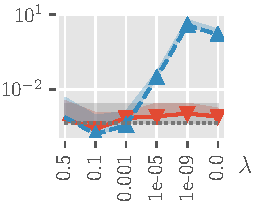
\includegraphics[height=0.18\textwidth]{img/likelihood_diff/banknote_authentication1_gauss_fullcov_likelihood_remain_retrain_f.pdf}
&
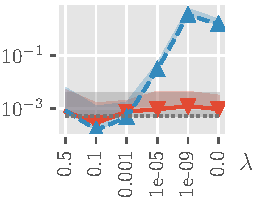
\includegraphics[height=0.17\textwidth]{img/likelihood_diff/banknote_authentication1_gauss_fullcov_likelihood_remove_retrain_f.pdf}
&
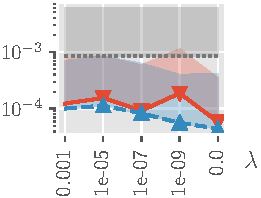
\includegraphics[height=0.17\textwidth]{img/likelihood_diff/banknote_authentication1_maf_likelihood_remain_retrain_f.pdf}
&
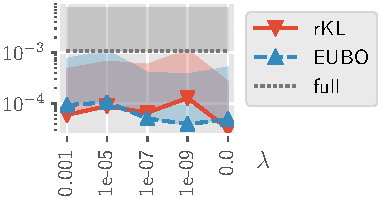
\includegraphics[height=0.17\textwidth]{img/likelihood_diff/banknote_authentication1_maf_likelihood_remove_retrain_f_legend.pdf}
\\
(a) $\dc$
&
(b) $\dr$
&
(c) $\dc$
&
(d) $\dr$
\end{tabular}\vspace{-2mm}
\caption{Graphs of averaged KL divergence vs.~$\lambda$ achieved by EUBO, rKL, and $q(\bm{\theta}|\da)$ (i.e., baseline labeled as \emph{full}) over $\dc$ and $\dr$ 
%with varying $\lambda$ 
for the banknote authentication dataset with the approximate posterior beliefs of model parameters represented by (a-b) multivariate Gaussians and (c-d) normalizing flows.}
\label{fig:authenresult}\vspace{-2.8mm}
\end{figure}
%
%\vspace{-1mm}
\subsection{Logistic Regression with Fashion MNIST Dataset}%\vspace{-1mm}
%
The fashion MNIST dataset of size $|\da| = 60000$ ($28\times28$ images of fashion items in $10$ classes) is partitioned into erased data of size $|\dr| = 10000$ and remaining data of size $|\dc| = 50000$.
The classification model is a neural network with $3$ fully-connected hidden layers of $128$, $128$, $64$ hidden neurons and a softmax layer to output the $10$-class probabilities.
The model can be interpreted as one of logistic regression on $64$ features generated from the hidden layer of $64$ neurons.
Since modeling all weights of the neural network as random variables can be costly, we model only $650$ weights in the transformation of the $64$ features to the inputs of the softmax layer.
The other weights remain constant during unlearning and retraining.
% As the number of weights in a neural network can be large, modeling all parameters in the network as random variables may be inefficient.
% Thus, we choose a simple approach that still allows unlearning. Only the weights of the last layer ($650$ weights) are modeled as random variables.
% When performing variational Bayesian unlearning, we keep the other weights constant and only compute the approximate unlearned posterior belief of these $650$ weights. 
% Thus, the output of the hidden layer of $64$ neurons are considered as features which are not unlearned.
% However, instead of being concerned with each weight of the network, we are more interested in the class probabilities (assessed via the marginal likelihood), which are used for prediction.
The prior beliefs of the network weights are $\mcl{N}(0, 10)$. The approximate posterior beliefs are modeled with independent Gaussians.
Though a large part of the network is fixed and we use simple models to represent the approximate posterior beliefs, we show that unlearning is still fairly effective.

As discussed in Sec.~\ref{subsec:expmoon},~\ref{subsec:experimentbanknote}, and Appendix~\ref{app:information}, the random selection of erased data $\dr$ and  redundancy in $\da$ lead to a small averaged KL divergence of about $0.1$ between $q(y_{\mbf{x}}|\da)$ vs.~$q(y_{\mbf{x}}|\dc)$ (i.e., baselines) over $\dc$ and $\dr$ (Figs.~\ref{fig:mnistresult}a and~\ref{fig:mnistresult}b) despite choosing a relatively large $|\dr|$.
Figs.~\ref{fig:mnistresult}a and~\ref{fig:mnistresult}b  show that when $\lambda \ge 10^{-9}$, EUBO and rKL achieve averaged KL divergences comparable to that of $q(\bm{\theta}|\da)$ (i.e., baseline labeled as \emph{full}), hence making their unlearning insignificant.\cref{log} 
%Based on the KL distances in , we observe that , the unlearning of both EUBO and rKL is insignificant as KL distances are similar to those . 
However, at $\lambda = 0$, the unlearning performance of rKL improves by achieving a smaller averaged KL divergence than that of $q(\bm{\theta}|\da)$, while EUBO's performance deteriorates.
Their performance can be further improved by using more complex models to represent their approximate posterior beliefs like that in Sec.~\ref{subsec:experimentbanknote}, albeit high-dimensional.
Figs.~\ref{fig:mnistresult}c and~\ref{fig:mnistresult}d show the class probabilities for two images evaluated at the mean of the approximate posterior beliefs with $\lambda = 0$. 
We observe that rKL induces the highest class probability for the same class as that of
$q(\bm{\theta}|\dc)$.
%the class probabilities induced by the rKL is observed to be similar to that of the re-trained posterior belief.
The class probabilities for other images 
%in $\da$ 
are shown in Appendix~\ref{app:fashionmnist}.
The two images 
%in Figs.~\ref{fig:mnistresult}c and~\ref{fig:mnistresult}d 
are taken from a separate  set of $10000$ test images (i.e., different from $\da$) where rKL with $\lambda = 0$ yields the same predictions as $q(\bm{\theta}|\dc)$ and $q(\bm{\theta}|\da)$ in, respectively, $99.34\%$ and $99.22\%$ of the test images, the latter of which are contained in the former.%\vspace{-1mm}
%among which consists of  same as the prediction of the full data posterior belief and $0.12\%$ different.
%
%
%
% \begin{figure}[h]
%     \centering
%     \begin{tabular}{@{}c@{}c@{}}
%     \includegraphics[height=0.17\textwidth]{img/likelihood_diff/fashionmnist_gauss_diag_likelihood_remain_retrain_f.pdf}
%     &
%     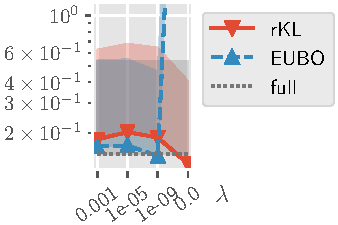
\includegraphics[height=0.17\textwidth]{img/likelihood_diff/fashionmnist_gauss_diag_likelihood_remove_retrain_f_legend.pdf}
%     \\
%     (a) $\dc$
%     &
%     (b) $\dr$
%     \end{tabular}
%     \caption{KL distances of EUBO, reverse KL (rKL), and $q(\bm{\theta}|\da)$ (\emph{full}) on $\dc$ and $\dr$ with varying $\lambda$ for the fashion MNIST dataset.}
%     \label{fig:mnistresult}
% \end{figure}
%
% \begin{figure}[ht]
% \centering
% \begin{tabular}{@{}c@{}c@{}}
% \makecell[t]{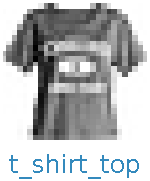
\includegraphics[width=0.11\textwidth]{img/fashionmnist/fashionmnist2_img_49937.eps}}
% &
% 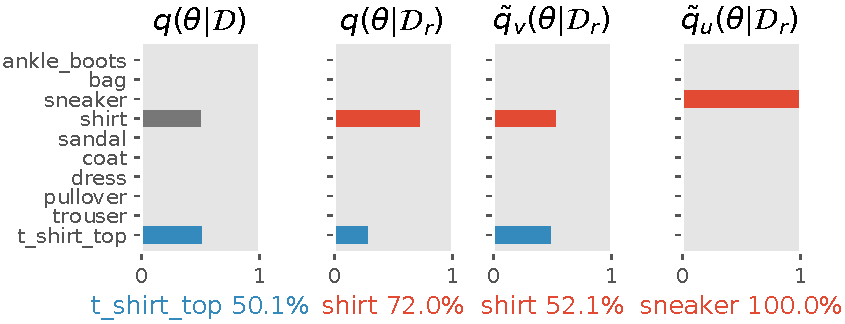
\includegraphics[width=0.65\textwidth]{img/fashionmnist/fashionmnist2_prob_49937.pdf}
% \end{tabular}
% \caption{Plot of the class probabilities from the approximate full-data, retrained, and unlearned posterior beliefs with $\lambda = 0$.}
% \label{fig:mnistdemo1}
% \end{figure}
%
\begin{figure}
\centering
\begin{tabular}{@{}c|c@{}c@{}}
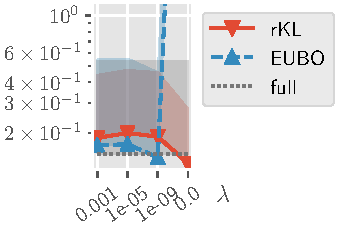
\includegraphics[width=0.3\textwidth]{img/likelihood_diff/fashionmnist_gauss_diag_likelihood_remain_retrain_f_legend.pdf}
&
\makecell[t]{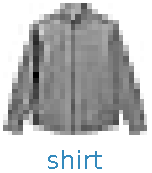
\includegraphics[width=0.07\textwidth]{img/fashionmnist/fashionmnist2_img_241.pdf}} % 49937
&
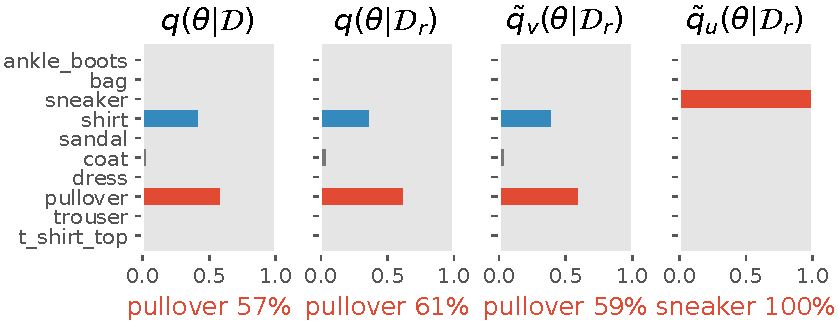
\includegraphics[width=0.55\textwidth]{img/fashionmnist/fashionmnist2_prob_241.pdf} % 49937
\\
(a) $\dc$ & \multicolumn{2}{c}{(c) Class probabilities for a `shirt' image}
\vspace{1mm}\\
%\vspace{3mm}\\
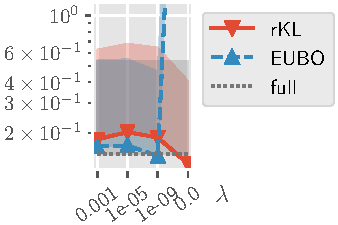
\includegraphics[width=0.3\textwidth]{img/likelihood_diff/fashionmnist_gauss_diag_likelihood_remove_retrain_f_legend.pdf}
&
\makecell[t]{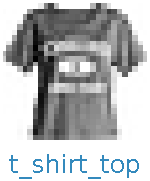
\includegraphics[width=0.07\textwidth]{img/fashionmnist/fashionmnist2_img_49937.pdf}} % 36790
&
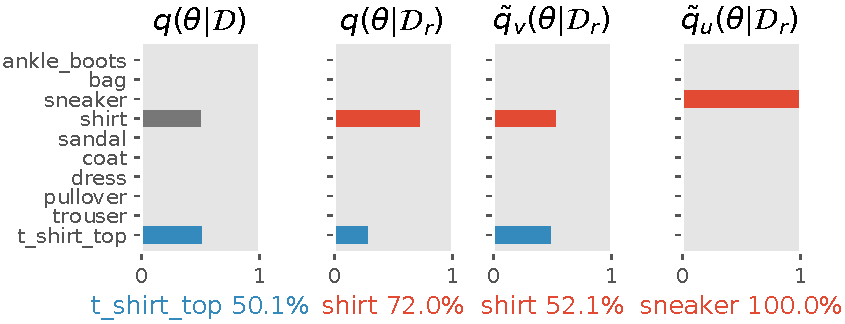
\includegraphics[width=0.55\textwidth]{img/fashionmnist/fashionmnist2_prob_49937.pdf} % 36790
\\
(b) $\dr$ & \multicolumn{2}{c}{(d) Class probabilities for a `T-shirt' image}
\end{tabular}%\vspace{-1mm}
\caption{Graphs of averaged KL divergence vs.~$\lambda$ achieved by EUBO, rKL, and $q(\bm{\theta}|\da)$ (i.e., baseline labeled as \emph{full}) over (a) $\dc$ and (b) $\dr$. (c-d) Plots of class probabilities for two images in the fashion MNIST dataset obtained using $q(\bm{\theta}|\da)$, $q(\bm{\theta}|\dc)$, optimized $\elbo(\bm{\theta}|\dc; \lambda = 0)$ and $\eubo(\bm{\theta}|\dc; \lambda = 0)$.}
\label{fig:mnistresult}%\vspace{-3mm}
\end{figure}
%
% \begin{figure}[ht]
% \centering
% \begin{tabular}{c|c}
% 	\makecell{
% 	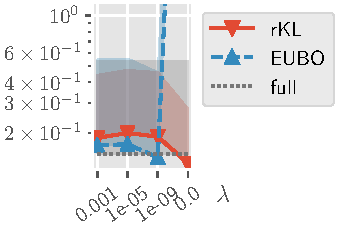
\includegraphics[trim={3mm 3mm 0mm 3mm}, clip,height=0.2\textwidth]{img/likelihood_diff/fashionmnist_gauss_diag_likelihood_remain_retrain_f_legend.pdf}
% 	\\
% 	(a) $\dc$
% 	\\
% 	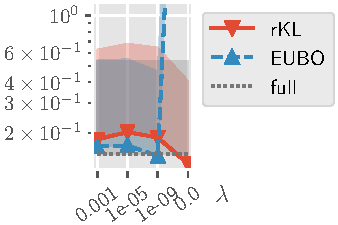
\includegraphics[trim={3mm 3mm 0mm 3mm}, clip,height=0.2\textwidth]{img/likelihood_diff/fashionmnist_gauss_diag_likelihood_remove_retrain_f_legend.pdf} 
% 	}
% 	&
% 	\makecell{
% 	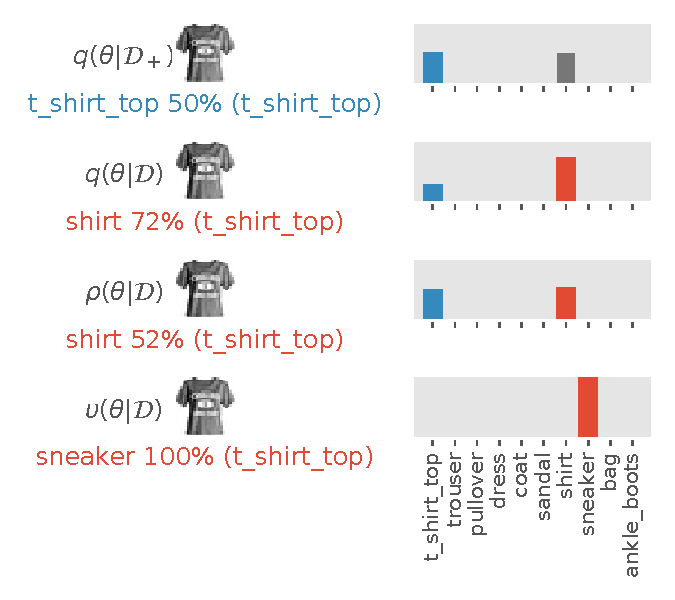
\includegraphics[height=0.4\textwidth]{img/fashionmnist/fashionmnist_49937.pdf}}
% 	\\
% 	(b) $\dr$
% 	&
% 	(c)
% \end{tabular}
% \caption{Plots of MAE of EUBO and rKL (a,b) and plot of the marginal likelihoods (i.e., class probabilities) from the approximate full-data, re-trained, and unlearned posterior beliefs with $\lambda = 0$) (c).}
% \label{fig:mnistresult}
% \end{figure}
%
%
\subsection{Sparse Gaussian Process (GP) Regression with Airline Dataset}%\vspace{-1mm}
\label{subsec:airline}
%
This section illustrates the scalability of unlearning to the massive airline dataset of $\sim 2$ million flights~\cite{hensman2013gaussian}. 
Training a sparse GP model with this massive dataset is made possible through stochastic VI~\cite{hensman2013gaussian}. 
Let $\mcl{X}_\mbf{u}$ denote the set of $50$ inducing inputs in the sparse GP model and $\mbf{f}_{\mcl{X}_\mbf{u}}$ be a vector of corresponding latent function values (i.e., inducing variables). The posterior belief $p(\mbf{f}_{\mcl{D}},\mbf{f}_{\mcl{X}_\mbf{u}}|\mcl{D})$ is approximated as $q(\mbf{f}_{\mcl{D}},\mbf{f}_{\mcl{X}_\mbf{u}}|\mcl{D}) \triangleq q(\mbf{f}_{\mcl{X}_\mbf{u}}|\mcl{D})\ p(\mbf{f}_{\mcl{D}}| \mbf{f}_{\mcl{X}_\mbf{u}})$ where $\mbf{f}_{\mcl{D}} \triangleq (f_{\mbf{x}})_{\mbf{x} \in \mcl{D}}$.
%denotes a vector of latent function values at the inputs of training data $\mcl{D}$. 
Let the sets $\mcl{X}_{\mcl{D}}$ and $\mcl{X}_{\dr}$ denote inputs in the full and erased data, respectively.
Then, the ELBO can be decomposed to
%
% \begin{equation}
% \hspace{-1.7mm}
% \begin{array}{rl}
% \displaystyle\mcl{L} &\hspace{-2.4mm}\displaystyle= \int q(\mbf{f}_{\mcl{X}_\mbf{u}}|\mcl{D})\left( \int p(\mbf{f}_{\mcl{D}}| \mbf{f}_{\mcl{X}_\mbf{u}}) \log p(\mbf{y}_{\mcl{D}}|\mbf{f}_{\mcl{D}})\ \text{d}\mbf{f}_{\mcl{D}} + \log \frac{p(\mbf{f}_{\mcl{X}_\mbf{u}})}{q(\mbf{f}_{\mcl{X}_\mbf{u}}|\mcl{D})} \right)\ \text{d}\mbf{f}_{\mcl{X}_\mbf{u}}\\
% 	&\hspace{-2.4mm}\displaystyle= \sum_{\mbf{x} \in \mcl{X}_{\mcl{D}}} \int q(\mbf{f}_{\mcl{X}_\mbf{u}}|\mcl{D})\  p(\mbf{f}_{\mbf{x}}| \mbf{f}_{\mcl{X}_\mbf{u}}) \log p(\mbf{y}_{\mbf{x}}|\mbf{f}_{\mbf{x}})\ \text{d}\mbf{f}_{\mbf{x}}\ \text{d}\mbf{f}_{\mcl{X}_\mbf{u}} 
% 	- \text{KL}\left[q(\mbf{f}_{\mcl{X}_\mbf{u}}|\mcl{D})\ \Vert\ p(\mbf{f}_{\mcl{X}_\mbf{u}})\right] %\int q(\mbf{f}_{\mcl{X}_\mbf{u}}|\mcl{D}) \log \frac{p(\mbf{f}_{\mcl{X}_\mbf{u}})}{q(\mbf{f}_{\mcl{X}_\mbf{u}}|\mcl{D})}\ \text{d}\mbf{f}_{\mcl{X}_\mbf{u}}
% \end{array}
% \label{eq:elbosvi}
% \end{equation}
%
\begin{equation}
\mcl{L} = \sum_{\mbf{x} \in \mcl{X}_{\mcl{D}}} \int q(\mbf{f}_{\mcl{X}_\mbf{u}}|\mcl{D})\  p(f_{\mbf{x}}| \mbf{f}_{\mcl{X}_\mbf{u}}) \log p(y_{\mbf{x}}|f_{\mbf{x}})\ \text{d}f_{\mbf{x}}\ \text{d}\mbf{f}_{\mcl{X}_\mbf{u}} 
	- \text{KL}[q(\mbf{f}_{\mcl{X}_\mbf{u}}|\mcl{D})\ \Vert\ p(\mbf{f}_{\mcl{X}_\mbf{u}})]
\label{eq:elbosvi}
\end{equation}
%
where $\int p(f_{\mbf{x}}| \mbf{f}_{\mcl{X}_\mbf{u}}) \log p(y_{\mbf{x}}|f_{\mbf{x}})\ \text{d}f_{\mbf{x}}$ can be evaluated in closed form~\cite{gal2014variational}.
To unlearn such a trained model from $\dr$ ($|\dr|=100$K here), the  EUBO~\eqref{eq:euboapprxadj} can be expressed in a similar way as the ELBO:
%
\begin{equation*}
\widetilde{\mcl{U}}_{\text{adj}}(\lambda)\hspace{-0.7mm}=\hspace{-1.2mm}\sum_{\mbf{x} \in \mcl{X}_{\dr}}\hspace{-1mm} \int\hspace{-0.7mm} \tilde{q}_u(\mbf{f}_{\mcl{X}_\mbf{u}}|\mcl{D}_r; \lambda) p(f_{\mbf{x}}| \mbf{f}_{\mcl{X}_\mbf{u}}) \log p_{\text{adj}}(y_{\mbf{x}}| f_{\mbf{x}}; \lambda)\ \text{d}f_{\mbf{x}}\ \text{d}\mbf{f}_{\mcl{X}_\mbf{u}} 
    \hspace{-0.5mm}+ \text{KL}[\eubo(\mbf{f}_{\mcl{X}_\mbf{u}}|\mcl{D}_r; \lambda) \Vert q(\mbf{f}_{\mcl{X}_\mbf{u}}|\mcl{D})]
%\label{eq:eubosvi}
\end{equation*}
%
where $p_{\text{adj}}(y_{\mbf{x}}| f_{\mbf{x}}; \lambda) = p(y_{\mbf{x}}| f_{\mbf{x}})$ if 
$q(f_{\mbf{x}},\mbf{f}_{\mcl{X}_\mbf{u}}|\mcl{D}) > \lambda \max_{\mbf{f}_{\mcl{X}_\mbf{u}}} q(f_{\mbf{x}},\mbf{f}_{\mcl{X}_\mbf{u}}|\mcl{D})$, 
%$q(\mbf{f}_{\mcl{X}_\mbf{u}}|\mcl{D}) > \lambda \max_{\mbf{f}_{\mcl{X}_\mbf{u}}} q(\mbf{f}_{\mcl{X}_\mbf{u}}|\mcl{D})$ 
%(i.e., $q(f_{\mbf{x}},\mbf{f}_{\mcl{X}_\mbf{u}}|\mcl{D}) > \lambda \max_{\mbf{f}_{\mcl{X}_\mbf{u}}} q(f_{\mbf{x}},\mbf{f}_{\mcl{X}_\mbf{u}}|\mcl{D})$)  
and $p_{\text{adj}}(y_{\mbf{x}}| f_{\mbf{x}}; \lambda) = 1$ otherwise.
% %
% \begin{equation*}
% p_{\text{adj}}(\mbf{y}_{\mbf{x}}|\mbf{f}_{\mbf{x}}; \lambda) \triangleq 
% 	\begin{cases}
% 		p(\mbf{y}_{\mbf{x}}|\mbf{f}_{\mbf{x}}) &\text{ if } q(\mbf{f}_{\mcl{X}_\mbf{u}}|\mcl{D}) > \lambda \max_{\mbf{f}_{\mcl{X}_\mbf{u}}} q(\mbf{f}_{\mcl{X}_\mbf{u}}|\mcl{D})\ ,\\
% 		1 &\text{ otherwise}\ .
% 	\end{cases}
% \end{equation*}
%
EUBO can be minimized using stochastic gradient descent with random subsets (i.e., mini-batches of size $10$K) of $\mcl{D}_e$ in each iteration. 
For rKL, we use the entire $\mcl{D}_e$ in each iteration.
%While the rKL expression in \eqref{eq:reversekl} is not decomposed as the EUBO is in \eqref{eq:eubosvi}, it is still a viable solution in practice as the erased dataset is often small.
%We unlearn the trained sparse GP model from an erased data $\mcl{D}_e$ of size~$100$K. 
%While EUBO is trained with mini-batches of $10$K data points in each iteration, rKL is trained with all erased data in each iteration. 
Since $\eubo(\mbf{f}_{\mcl{X}_\mbf{u}}| \mcl{D}_r; \lambda)$, $\elbo(\mbf{f}_{\mcl{X}_\mbf{u}}| \mcl{D}_r; \lambda)$, and $q(\mbf{f}_{\mcl{X}_\mbf{u}}| \mcl{D}_r)$  in~\eqref{eq:elbosvi}~\cite{gal2014variational} are all multivariate Gaussians,
%the approximate posterior beliefs of $\mbf{f}_{\mcl{X}_\mbf{u}}$ are multivariate Gaussians. Since it is known the posterior belief of $\mbf{f}_{\mcl{X}_\mbf{u}}$ maximizing ELBO in~\eqref{eq:elbosvi} is a multivariate Gaussian~\cite{gal2014variational}, 
we can directly evaluate the  performance of EUBO and rKL with varying $\lambda$ through their respective $\text{KL}[\eubo(\mbf{f}_{\mcl{X}_\mbf{u}}| \mcl{D}_r; \lambda)\ \Vert\ q(\mbf{f}_{\mcl{X}_\mbf{u}}| \mcl{D}_r)]$ and $\text{KL}[\elbo(\mbf{f}_{\mcl{X}_\mbf{u}}| \mcl{D}_r; \lambda)\ \Vert\ q(\mbf{f}_{\mcl{X}_\mbf{u}}| \mcl{D}_r)]$ which, according to Table~\ref{tbl:airlineresult}, are smaller than $\text{KL}[q(\mbf{f}_{\mcl{X}_\mbf{u}}| \mcl{D})\ \Vert\ q(\mbf{f}_{\mcl{X}_\mbf{u}}| \mcl{D}_r)]$ of value $4344.09$ (i.e., baseline representing no unlearning), hence demonstrating reasonable unlearning performance.
%
%the KL divergence of $4344.09$ between the posterior belief $q(\mbf{f}_{\mcl{X}_\mbf{u}}| \mcl{D})$ given full data $\mcl{D}$ and $q(\mbf{f}_{\mcl{X}_\mbf{u}}| \mcl{D}_r)$ obtained from retraining with remaining data $\mcl{D}_r$ for varying values of $\lambda$.
%Both EUBO and rKL demonstrate reasonable performance as observed in Table~\ref{tbl:airlineresult}: the KL divergences from EUBO and rKL for $\lambda \in \{10^{-11}, 10^{-13}, 10^{-20}, 0\}$ are smaller than the KL divergence between the posterior belief $q(\mbf{f}_{\mcl{X}_\mbf{u}}| \mcl{D})$ given full data $\mcl{D}$ and $q(\mbf{f}_{\mcl{X}_\mbf{u}}| \mcl{D}_r)$ obtained from retraining with remaining data $\mcl{D}_r$ which is $4344.09$.
%
% \begin{table}
% \centering
% \label{tbl:airlineresult}
% \caption{The KL divergences between posterior beliefs unlearned from erased data $\dr$ and that obtained from VI training with remaining data $\dc$.}
% \begin{tabular}{ccc}
% \toprule
% $\lambda$ & $\text{KL}[\eubo(\mbf{f}_{\mcl{X}_\mbf{u}}| \mcl{D}_r; \lambda)\ \Vert\ q(\mbf{f}_{\mcl{X}_\mbf{u}}| \mcl{D}_r)]$ & $\text{KL}[\elbo(\mbf{f}_{\mcl{X}_\mbf{u}}| \mcl{D}_r; \lambda)\ \Vert\ q(\mbf{f}_{\mcl{X}_\mbf{u}}| \mcl{D}_r)]$\\
% \midrule
% $10^{-11}$ & $2194.49$ & $418.42$ \\
% $10^{-13}$ & $1943.00$ & $367.12$ \\
% $10^{-20}$ & $1384.96$ & 	$543.45$ \\
% $0$ & $2629.71$ & $455.11$ \\
% \bottomrule
% \end{tabular}
% \end{table}
%
\begin{table}
\centering
\caption{KL divergence achieved by EUBO (top row) and rKL (bottom row)
%between posterior beliefs unlearned from erased data $\dr$ and that obtained using VI from retraining with remaining data $\dc$ 
with varying $\lambda$ for airline dataset.}
\begin{tabular}{ccccc}
\toprule
$\lambda$ &  $10^{-11}$ & $10^{-13}$ & $10^{-20}$ & $0$\\
\midrule
$\text{KL}[\eubo(\mbf{f}_{\mcl{X}_\mbf{u}}| \mcl{D}_r; \lambda)\ \Vert\ q(\mbf{f}_{\mcl{X}_\mbf{u}}| \mcl{D}_r)]$
& $2194.49$ & $1943.00$ & $1384.96$ & $2629.71$
\\
$\text{KL}[\elbo(\mbf{f}_{\mcl{X}_\mbf{u}}| \mcl{D}_r; \lambda)\ \Vert\ q(\mbf{f}_{\mcl{X}_\mbf{u}}| \mcl{D}_r)]$
& $418.42$ & $367.12$ & $543.45$ & $455.11$ \\
\bottomrule
\end{tabular}
%\vspace{-3mm}
\label{tbl:airlineresult}
\end{table}
%
%Full vs remain
%[[4344.08637021]]
%EUBO train 3000, batch 10k
%{0.0: array([[2629.71293337]]), 0.001: array([[30338.74120233]]), 1e-05: array([[29035.10966532]]), 1e-09: array([[265140.14311844]]), 1e-15: array([[45363.68117277]]), 1e-11: array([[2194.49011088]]), 1e-20: array([[1384.96127853]]), 1e-13: array([[1943.00193635]])}
%ELBO train 3000, batch 10k
%{0.0: array([[547.35207073]]), 0.001: array([[545.4468024]]), 1e-05: array([[470.38541202]]), 1e-09: array([[669.09307346]]), 1e-15: array([[324.49970775]]), 1e-11: array([[462.37658397]]), 1e-20: array([[495.92322004]]), 1e-13: array([[393.58787182]])}
%ELBO train 1000, batch 100k
%{0.0: array([[455.11289995]]), 1e-15: array([[329.8596652]]), 1e-11: array([[418.41791927]]), 1e-20: array([[543.44544525]]), 1e-13: array([[367.12024594]])}
%
\section{Conclusion}
\label{sec:conclusion}%\vspace{-1mm}
%
This paper describes novel  unlearning methods for approximately unlearning a Bayesian model from a small subset of training data to be erased. Our unlearning methods are parsimonious in requiring only the approximate posterior belief of model parameters given the full data (i.e., obtained in model training with VI) and erased data to be available. This makes unlearning even more challenging due to two sources of inaccuracy in the approximate posterior belief.
We introduce novel tricks of adjusted likelihood and reverse KL to curb unlearning in the region of model parameters with low approximate posterior belief where both sources of inaccuracy primarily occur.
%investigates the Bayesian unlearning problem, i.e., erasing a small subset of the training data from a Bayesian model. When the exact full-data posterior belief is available, we propose EUBO, which is a counterpart of ELBO in the conventional VI. Minimizing EUBO can effectively produce an approximate unlearned posterior belief that minimizes its KL divergence to the exact posterior belief given the remaining data. Furthermore, the expression of EUBO can be interpreted as balancing between fully unlearning from erased data and not entirely forgetting the exact posterior belief given the full data.
%When there is only an approximate full-data posterior belief obtained from model training with VI, we introduce the adjusted likelihood to avoid the undesired consequence of directly applying our EUBO approach. Moreover, we introduce another trick that minimizes the reverse KL without needing the adjusted likelihood.
Empirical evaluations on synthetic and real-world datasets show that our proposed methods (especially reverse KL without adjusted likelihood) can effectively unlearn Bayesian models such as sparse GP and logistic regression from erased data.
%The performance of the proposed approaches is empirically shown in several Bayesian models including sparse GP and logistic regression with the approximate posterior belief modeled by a normalizing flow.
% In practice, our unlearning approaches can be used to fulfill the limited time requirement for unlearning while retaining the usability of the model. 
In practice, for the approximate posterior beliefs recovered by unlearning from erased data using our proposed methods, they can be immediately used in ML applications and continue to be improved at the same time
%To further improve the unlearned model after unlearning, a practical approach is to continue to fine-tuning the unlearned posterior belief 
by retraining with the remaining data at the expense of parsimony.
In our future work, we will apply our our proposed methods to unlearning more sophisticated Bayesian models like the entire family of sparse GP models~\cite{Chen13,LowTASE15,LowRSS13,LowUAI12,MinhAAAI17,HoangICML19,hoang2015unifying,HoangICML16,NghiaAAAI19,LowECML14a,low15,Ruofei18,teng20,LowAAAI14,HaibinAPP}) and deep GP models~\cite{yu19}.

\clearpage
\section*{Broader Impact}

% Authors are required to include a statement of the broader impact of their work, including its ethical aspects and future societal consequences. 
% Authors should discuss both positive and negative outcomes, if any. For instance, authors should discuss a) 
% who may benefit from this research, b) who may be put at disadvantage from this research, c) what are the consequences of failure of the system, and d) whether the task/method leverages
% biases in the data. If authors believe this is not applicable to them, authors can simply state this.

As discussed in our introduction (Sec.~\ref{sec:intro}), a direct contribution of our work to the society in this information age is to the implementation of \emph{personal data ownership} (i.e., enforced by the General Data Protection Regulation in the European Union \cite{mantelero2013eu}) by studying the problem of machine unlearning for Bayesian models. Such an implementation can boost the confidence of users about sharing their data with an application/organization when they know that the trace of their data can be reduced/erased, as requested.
As a result, organizations/applications can gather more useful data from users to enhance their service back to the users and hence to the society.

Our unlearning work can also contribute to the defense against data poisoning attacks (i.e., injecting malicious training data). Instead of retraining the tampered machine learning model from scratch to recover the quality of a service, unlearning the model from the detected malicious data may incur much less time, which improves the user experience and reduces the cost due to the service disruption.

In contrast, the ability to unlearn machine learning models may also open the door to new adversarial activities. For example, in the context of data sharing, multiple parties share their data to train a common machine learning model. An unethical party can deliberately share a low-quality dataset instead of its high-quality one. After obtaining the model trained on datasets from all parties (including the low-quality dataset), the unethical party can unlearn the low-quality dataset and continue to train the model with its high-quality dataset.
By doing this, the unethical party achieves a better model than other parties in the collaboration. Therefore, the possibility of machine unlearning should be considered in the design of different data sharing frameworks.

% Lastly, one should be aware of the limitation of our work to avoid undesired consequences, especially when the exact posterior belief of the model parameters given the full data is not available. 
% % completeness
% In this case, the approximation in the posterior belief given the full data makes it challenging for our method to perform exact unlearning. 
% Thus, if exact Bayesian unlearning is required with a time constraint, one should choose a model that allows learning an exact posterior belief.
% On the other hand, in practice, an application may need an efficient unlearning method (in terms of time and data) to satisfy the constraint on the response time to the user request, without rendering the model useless (e.g., catastrophic unlearning). 
% After processing the unlearning request, the application can continue to fine-tune the unlearned model by retraining on the remaining data, which results in better unlearning quality at the expense of time and data.
% It is a scenario that our proposed methods fit. Our work also motivates a future research direction of maintaining additional information about the approximate posterior belief in the VI training to improve the unlearning quality.

\begin{ack}
This research/project is supported by the National Research Foundation, Singapore under its Strategic Capability Research Centres Funding Initiative. Any opinions, findings and conclusions or recommendations expressed in this material are those of the author(s) and do not reflect the views of National Research Foundation, Singapore.
\end{ack}

%\begin{small}
    \bibliographystyle{abbrv}
    \bibliography{unlearn}
%\end{small}

\clearpage
\appendix 
%
%\section{Description of the Gaussian with Unknown Mean Example}
%\label{app:gum}
%
%%$60$ data points, prior distribution is a mixture $0.5 \mcl{N}(0.0, 1.0) + 0.5 \mcl{N}(4.0, 1.0)$, likelihood is $\mcl{N}(1.0, \sigma^2=100)$.
%%
%%Removing $10$ largest data points.
%
%\section{Adjusted Posterior}
%
%
%\begin{align*}
%\log p(\dr|\dc) &= \log \frac{p(\dr|\bm{\theta}, \dc)p(\bm{\theta}|\dc)}{p(\bm{\theta}|\da)}\\
%\log C	&= \log \frac{p(\dr|\bm{\theta}, \dc) \tilde{p}(\bm{\theta}|\dc)}{q(\bm{\theta}|\da)}\\
%\int \tilde{p}(\bm{\theta}|\dc) \log C\ \text{d}\bm{\theta}	&= \int \tilde{p}(\bm{\theta}|\dc) \log \frac{p(\dr|\bm{\theta},\dc) \tilde{p}(\bm{\theta}|\dc) q(\bm{\theta}|\dc)}{q(\bm{\theta}|\dc) q(\bm{\theta}|\da)}\ \text{d}\bm{\theta}\\
%	&= \int \tilde{p}(\bm{\theta}|\dc) \log p(\dr|\bm{\theta},\dc)\ \text{d}\bm{\theta}
%	+ \text{KL}[\tilde{p}(\bm{\theta}|\dc)\ \Vert\ q(\bm{\theta}|\dc)]
%	+ \int \tilde{p}(\bm{\theta}|\dc) \log \frac{q(\bm{\theta}|\dc)}{q(\bm{\theta}|\da)}\ \text{d}\bm{\theta}\\
%\log C - \text{KL}[\tilde{p}(\bm{\theta}|\dc)\ \Vert\ q(\bm{\theta}|\dc)]
%	&= \int \tilde{p}(\bm{\theta}|\dc) \log p(\dr|\bm{\theta},\dc)\ \text{d}\bm{\theta}
%	+ \int \tilde{p}(\bm{\theta}|\dc) \log \frac{q(\bm{\theta}|\dc)}{q(\bm{\theta}|\da)}\ \text{d}\bm{\theta}\\
%	&= C \left[ 
%		\int \frac{q(\bm{\theta}|\da)}{p(\dr|\bm{\theta},\dc)} \log p(\dr|\bm{\theta},\dc)\ \text{d}\bm{\theta}
%		+ \int \frac{q(\bm{\theta}|\da)}{p(\dr|\bm{\theta},\dc)} \log \frac{q(\bm{\theta}|\dc)}{q(\bm{\theta}|\da)}\ \text{d}\bm{\theta}
%	\right]
%\end{align*}
%%
%where $\tilde{p}(\bm{\theta}|\dc) \triangleq C q(\bm{\theta}|\da) / p(\dr|\bm{\theta}, \dc)$.
%\todo{implementation: need to scale up the lower bound so that the value is sufficiently large} \todo{we need to plot $\tilde{p}(\bm{\theta}|\dc)$}.
%restrict $q(\bm{\theta}|\da)$ to region of high probability.
%
%\todo{no need for VI above, just directly optimize the KL divergence}
%
%\begin{align*}
%\int q(\bm{\theta}|\dc) \log C\ \text{d}\bm{\theta}	&= \int q(\bm{\theta}|\dc) \log \frac{p(\dr|\bm{\theta},\dc) \tilde{p}(\bm{\theta}|\dc) q(\bm{\theta}|\dc)}{q(\bm{\theta}|\dc) q(\bm{\theta}|\da)}\ \text{d}\bm{\theta}\\
%\log C + \text{KL}[q(\bm{\theta}|\dc)\ \Vert\ \tilde{p}(\bm{\theta}|\dc)]
%	&= \int q(\bm{\theta}|\dc) \log \frac{p(\dr|\bm{\theta},\dc) q(\bm{\theta}|\dc)}{q(\bm{\theta}|\da)}\ \text{d}\bm{\theta}\\
%	&= \int q(\bm{\theta}|\dc) \log p(\dr|\bm{\theta},\dc)\ \text{d}\bm{\theta}
%	+ \text{KL}[q(\bm{\theta}|\dc)\ \Vert\ q(\bm{\theta}|\da)]
%\end{align*}
%
%by adjusting $q(\bm{\theta}|\da)$ we consistently adjust both the LHS and RHS of the above 2 equations. However, with EUBO formation, setting $q(\bm{\theta}|\da) = 0$ requires $q(\bm{\theta}|\dc) = 0$, while it is not necessary for ELBO formulation. Furthermore, for EUBO formulation, we cannot adjust the posterior $q(\bm{\theta}|\da)$ because optimizing $q(\bm{\theta}|\dc)$ might focus more mass on the constant term! This is not true for the ELBO approach.
%
\section{Proof of Proposition~\ref{rmk:klmarginal}}
\label{app:klmarginal}
%
%This section shows the inequality in Remark~\ref{rmk:klmarginal}.
We first follow the proof of the log-sum inequality to prove the following inequality:
%
% \begin{equation}
% \mbb{E}_{q(\bm{\theta}|\dc)}[p(\mbf{y}|\bm{\theta})]\ \log \frac{\mbb{E}_{q(\bm{\theta}|\dc)}[p(\mbf{y}|\bm{\theta})]}{\mbb{E}_{p(\bm{\theta}|\dc)}[p(\mbf{y}|\bm{\theta})]}
% \le \int q(\bm{\theta}|\dc)\  p(\mbf{y}|\bm{\theta})\ \log \frac{q(\bm{\theta}|\dc)}{p(\bm{\theta}|\dc)}\ \text{d}\bm{\theta}
% \label{eq:logsum2}
% \end{equation}
%
\begin{equation}
q_u(y|\dc)\ \log \frac{q_u(y|\dc)}{p(y|\dc)}
\le \int q_u(\bm{\theta}|\dc)\  p(y|\bm{\theta})\ \log \frac{q_u(\bm{\theta}|\dc)}{p(\bm{\theta}|\dc)}\ \text{d}\bm{\theta}
\label{eq:logsum2}
\end{equation}
%
where $q_u(y|\dc) \triangleq \mbb{E}_{q_u(\bm{\theta}|\dc)}[p(y|\bm{\theta})] = \int q_u(\bm{\theta}|\dc)\  p(y|\bm{\theta})\ \text{d}\bm{\theta}$ and $p(y|\dc) \triangleq \mbb{E}_{p(\bm{\theta}|\dc)}[p(y|\bm{\theta})] = \int p(\bm{\theta}|\dc)\  p(y|\bm{\theta})\ \text{d}\bm{\theta}$.
%
\begin{proof}
Define the function $f(t) \triangleq t\log t$ which is convex. Then, 
%
\begin{align*}
&\int q_u(\bm{\theta}|\dc)\  p(y|\bm{\theta})\ \log \frac{q_u(\bm{\theta}|\dc)}{p(\bm{\theta}|\dc)}\ \text{d}\bm{\theta}\\
&=\int p(\bm{\theta}|\dc) \ p(y|\bm{\theta})\  f\left(\frac{q_u(\bm{\theta}|\dc)}{p(\bm{\theta}|\dc)}\right)\ \text{d}\bm{\theta}\\
&=\mbb{E}_{p(\bm{\theta}|\dc)}[p(y|\bm{\theta})] 
    \int 
    \frac{p(\bm{\theta}|\dc) \ p(y|\bm{\theta})}{\mbb{E}_{p(\bm{\theta}|\dc)}[p(y|\bm{\theta})]}\ 
    f\left(\frac{q_u(\bm{\theta}|\dc)}{p(\bm{\theta}|\dc)}\right)\ \text{d}\bm{\theta}\\
&\ge \mbb{E}_{p(\bm{\theta}|\dc)}[p(y|\bm{\theta})] 
    \ f\left(
        \int 
        \frac{p(\bm{\theta}|\dc) \ p(y|\bm{\theta})}{\mbb{E}_{p(\bm{\theta}|\dc)}[p(y|\bm{\theta})]}
        \frac{q_u(\bm{\theta}|\dc)}{p(\bm{\theta}|\dc)}\ \text{d}\bm{\theta}
    \right)\\
&= \mbb{E}_{p(\bm{\theta}|\dc)}[p(y|\bm{\theta})] 
\ f\left(
        \int 
        \frac{p(y|\bm{\theta})\ q_u(\bm{\theta}|\dc)}{\mbb{E}_{p(\bm{\theta}|\dc)}[p(y|\bm{\theta})]}\ \text{d}\bm{\theta}
    \right)\\
&= \mbb{E}_{p(\bm{\theta}|\dc)}[p(y|\bm{\theta})] 
    \ f\left(
        \frac{ \mbb{E}_{q_u(\bm{\theta}|\dc)}[p(y|\bm{\theta})]}{\mbb{E}_{p(\bm{\theta}|\dc)}[p(y|\bm{\theta})]}
    \right)\\
&= \mbb{E}_{q_u(\bm{\theta}|\dc)}[p(y|\bm{\theta})]\ \log \frac{\mbb{E}_{q_u(\bm{\theta}|\dc)}[p(y|\bm{\theta})]}{\mbb{E}_{p(\bm{\theta}|\dc)}[p(y|\bm{\theta})]}\\
&= q_u(y|\dc)\ \log \frac{q_u(y|\dc)}{p(y|\dc)}
\end{align*}
where the inequality is due to Jensen's inequality.
\end{proof}

Then, integrating both sides of \eqref{eq:logsum2} w.r.t.~$y$, 
%
\begin{align*}
\int q_u(y|\dc)\ \log \frac{q_u(y|\dc)}{p(y|\dc)}\ \text{d}y
&\le 
\int \int q_u(\bm{\theta}|\dc) \ p(y|\bm{\theta})\ \log \frac{q_u(\bm{\theta}|\dc)}{p(\bm{\theta}|\dc)}\ \text{d}\bm{\theta}\ \text{d}y\\
\int q_u(y|\dc)\ \log \frac{q_u(y|\dc)}{p(y|\dc)}\ \text{d}y
&\le 
\int q_u(\bm{\theta}|\dc) \left(\int p(y|\bm{\theta})\ \text{d}y \right) \log \frac{q_u(\bm{\theta}|\dc)}{p(\bm{\theta}|\dc)}\ \text{d}\bm{\theta}\\
\int q_u(y|\dc)\ \log \frac{q_u(y|\dc)}{p(y|\dc)}\ \text{d}y
&\le 
\int q_u(\bm{\theta}|\dc) \log \frac{q_u(\bm{\theta}|\dc)}{p(\bm{\theta}|\dc)}\ \text{d}\bm{\theta}\\
\text{KL}[q_u(y|\dc)\ \Vert\ p(y|\dc)] &\le \text{KL}[q_u(\bm{\theta}|\dc)\ \Vert\ p(\bm{\theta}|\dc)]\ .
\end{align*}

\section{Proof of Proposition~\ref{theo:eubo}}
\label{app:eubo}
%
%Let $q(\bm{\theta}|\dc)$ be the probability density of a distribution over $\bm{\theta}$ (the notation $\dc$ in $q(\bm{\theta}|\dc)$ is only to differentiate $q(\bm{\theta}|\dc)$ with $q(\bm{\theta}|\da)$).
From \eqref{eq:suffdata}, 
%
\begin{align*}
\log p(\dr|\dc) &= \log \frac{p(\dr|\bm{\theta})\ p(\bm{\theta}|\dc)}{p(\bm{\theta}|\da)}\\
    &= \log \frac{q_u(\bm{\theta}|\dc)\ p(\dr|\bm{\theta})\  p(\bm{\theta}|\dc)}{q_u(\bm{\theta}|\dc)\  p(\bm{\theta}|\da)}\\
    &= \log p(\dr|\bm{\theta})
    + \log \frac{q_u(\bm{\theta}|\dc)}{p(\bm{\theta}|\da)}
    - \log \frac{q_u(\bm{\theta}|\dc)}{p(\bm{\theta}|\dc)}\ .
\end{align*}
%
Then, taking an expectation of both sides w.r.t.~$q_u(\bm{\theta}|\dc)$,
%
\begin{align*}
\log p(\dr|\dc) &=
    \int q_u(\bm{\theta}|\dc) \log p(\dr|\bm{\theta})\ \text{d}\bm{\theta}
    + \int q_u(\bm{\theta}|\dc) \log \frac{q_u(\bm{\theta}|\dc)}{p(\bm{\theta}|\da)}\ \text{d}\bm{\theta}
    - \int q_u(\bm{\theta}|\dc) \log \frac{q_u(\bm{\theta}|\dc)}{p(\bm{\theta}|\dc)}\ \text{d}\bm{\theta}\\
    &= \int q_u(\bm{\theta}|\dc)\  \log p(\dr|\bm{\theta})\ \text{d}\bm{\theta}
    + \text{KL}[q_u(\bm{\theta}|\dc)\ \Vert\ p(\bm{\theta}|\da)]
    - \text{KL}[q_u(\bm{\theta}|\dc)\ \Vert\ p(\bm{\theta}|\dc)]\\
    &= \mcl{U} - \text{KL}[q_u(\bm{\theta}|\dc)\ \Vert\ p(\bm{\theta}|\dc)]\ .
\end{align*}
%
Therefore,
%
\begin{align*}
\mcl{U} =  \log p(\dr|\dc) + \text{KL}[q_u(\bm{\theta}|\dc)\ \Vert\ p(\bm{\theta}|\dc)] \ge \log p(\dr|\dc)
\end{align*}
%
since $\text{KL}[q_u(\bm{\theta}|\dc)\ \Vert\ p(\bm{\theta}|\dc)] \ge 0$.
So, $\mcl{U}$ is an upper bound of $\log p(\dr|\dc)$.
%
\section{Bayesian Linear Regression}
\label{app:lr}
%
We perform unlearning of a simple Bayesian linear regression model: $y_x = ax^3 + bx^2 + cx + d + \epsilon$ where $a=2$, $b=-3$, $c=1$, and $d=0$ are the model parameters $\bm{\theta}$, and the noise is $\epsilon \sim \mcl{N}(0,0.05^2)$. 
Though the exact posterior belief of $\bm{\theta}$ is known to be a multivariate Gaussian, we choose to use a low-rank approximation (i.e.,  multivariate Gaussian with a diagonal covariance matrice) and represent the approximate posterior beliefs of the model parameters with independent Gaussians 
%Although it is known that the posterior beliefs are multivariate Gaussians, the low-rank approximation of the posterior beliefs are chosen as diagonal Gaussians
so that the approximation is not exact.

Fig.~\ref{fig:lrkl}a shows the remaining data $\dc$ and erased data $\dr$. Note that the erased data $\dr$ is informative to the approximate posterior beliefs of the model parameters $\bm{\theta}$ as $\dr$ are clustered. So, the difference between the samples drawn from predictive distributions $q(y_x| \da)$ (Fig.~\ref{fig:lrkl}b) vs.~$q(y_x| \dc)$ (Fig.~\ref{fig:lrkl}c) is large.
%
\begin{table}[h]
\centering
\caption{KL divergences achieved by EUBO (left column) and rKL (right column) with varying $\lambda$ for synthetic linear regression dataset.}
\begin{tabular}{ccc}
\toprule
$\lambda$ & $\text{KL}[\eubo(\bm{\theta}|\dc;\lambda)\ \Vert\ q(\bm{\theta}|\dc)]$ & $\text{KL}[\elbo(\bm{\theta}|\dc;\lambda)\ \Vert\ q(\bm{\theta}|\dc)]$\\
\midrule
$0.5$ & $0.1143$ & $0.1012$\\
$0.1$ & $0.0899$ & $0.0600$\\
$0.0$ & $266.68$ & $0.0158$\\
\bottomrule
\end{tabular}
\label{tbl:lrkl}
\end{table}
%
\begin{figure}
\centering
\begin{tabular}{ccc}
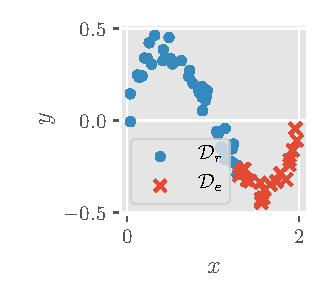
\includegraphics[height=0.2\textwidth]{img/linear_regression/lr_data}
&
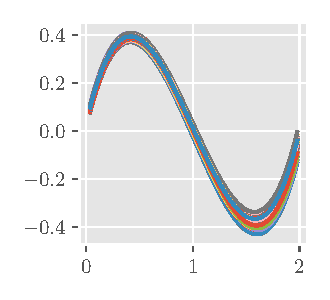
\includegraphics[height=0.2\textwidth]{img/linear_regression/linear_regression_gauss_diag_full}
&
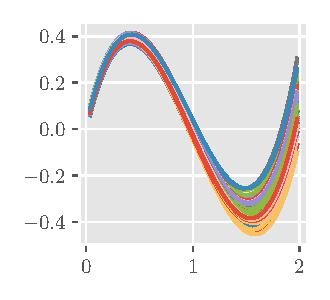
\includegraphics[height=0.2\textwidth]{img/linear_regression/linear_regression_gauss_diag_remain}
\\
(a) Dataset
&
(b) Samples from $q(y_x| \da)$
&
(c) Samples from $q(y_x| \dc)$
\\
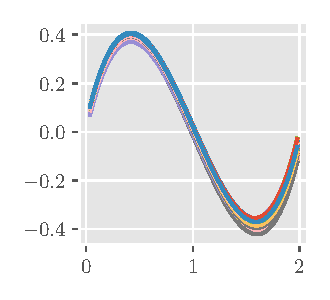
\includegraphics[height=0.2\textwidth]{img/linear_regression/linear_regression_gauss_diag_eubo_0_5}
&
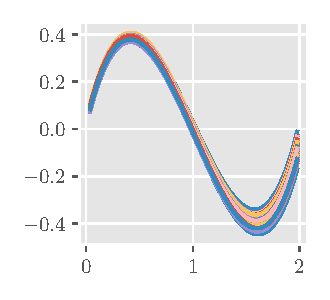
\includegraphics[height=0.2\textwidth]{img/linear_regression/linear_regression_gauss_diag_eubo_0_1}
&
\includegraphics[height=0.2\textwidth]{img/linear_regression/linear_regression_gauss_diag_eubo_0_0}
\\
(d) EUBO with $\lambda = 0.5$
&
(e) EUBO with $\lambda = 0.1$
&
(f) EUBO with $\lambda = 0$
\\
\includegraphics[height=0.2\textwidth]{img/linear_regression/linear_regression_gauss_diag_elbo_0_5}
&
\includegraphics[height=0.2\textwidth]{img/linear_regression/linear_regression_gauss_diag_elbo_0_1}
&
\includegraphics[height=0.2\textwidth]{img/linear_regression/linear_regression_gauss_diag_elbo_0_0}
\\
(g) rKL with $\lambda = 0.5$
&
(h) rKL with $\lambda = 0.1$
&
(i) rKL with $\lambda = 0$
\end{tabular}
\caption{Plots of (a) synthetic linear regression dataset with erased data $\dr$ (crosses) and remaining data $\dc$ (dots), and samples from predictive distributions obtained using VI from (b) training with full data $\da$ and (c) retraining with $\dc$. Plots of samples from predictive distributions (d-f) $\eubo(y_x|\dc)$ and (g-i) $\elbo(y_x|\dc)$ induced, respectively, by EUBO and rKL with varying $\lambda$.}
\label{fig:lrkl}
\end{figure}

From Table~\ref{tbl:lrkl}, the KL divergences achieved by EUBO and rKL with $\lambda =0.1, 0.5$ are smaller than $\text{KL}[q(\bm{\theta}|\da)\ \Vert\ q(\bm{\theta}|\dc)]$ of value $0.1170$ (i.e., baseline representing no unlearning), hence demonstrating reasonable unlearning performance.
%Both EUBO and rKL demonstrate reasonable performance as observed in Table~\ref{tbl:lrkl}: the KL divergences from EUBO and rKL for $\lambda \in \{0.1, 0.5\}$ are smaller than the KL divergence  between the posterior belief $q(\bm{\theta}|\da)$ given full data $\da$ and $q(\bm{\theta}|\dc)$ obtained using VI from retraining with remaining data $\dc$ which is $0.1170$. 
When $\lambda = 0$, EUBO suffers from catastrophic unlearning, but rKL does not.
The KL divergences in Table~\ref{tbl:lrkl} also agree with the plots of samples drawn from the predictive distributions induced by EUBO and rKL in Fig.~\ref{fig:lrkl} by comparing with the samples drawn from the predictive distribution obtained using VI from retraining with $\dc$ in Fig.~\ref{fig:lrkl}c.
%
\section{Bimodal Posterior Belief}
\label{app:multimode}
%
Let the posterior belief of model parameter $\theta$ given full data $\da$ be a Gaussian mixture (i.e., a bimodal distribution): 
\begin{equation}
p(\theta|\da) \triangleq 0.5\ \phi(\theta; 0,1) + 0.5\ \phi(\theta; 2,1)
\label{eq:mmfullpost}
\end{equation}
%
where $\phi(\theta;\mu,\sigma^2)$ is a Gaussian p.d.f.~with mean $\mu$ and variance $\sigma^2$.
%
We deliberately choose the likelihood of the erased data $\dr$ to be
%
\begin{equation}
p(\dr|\theta) \triangleq 1 + \frac{\phi(\theta;2,1)}{\phi(\theta;0,1)}
\label{eq:mmerasedll}
\end{equation}
%
so that the posterior belief of $\theta$ given the remaining data $\dc$ is a Gaussian:
%
\begin{equation}
p(\theta|\dc) \propto \frac{p(\theta|\da)}{p(\dr|\theta)}
	= \phi(\theta; 0,1)
\label{eq:mmremainpost}
\end{equation}
%
where the proportionality is due to~\eqref{eq:suffdata}.

We assume to only have access to the likelihood of the erased data in~\eqref{eq:mmerasedll}; the exact posterior beliefs of $\theta$ given the full data~\eqref{eq:mmfullpost} and that given the remaining data \eqref{eq:mmremainpost} are not available. Instead, we have access to an approximate posterior belief $q(\theta|\da)$ given the full data obtained using VI by minimizing $\text{KL}[q(\theta|\da)\ \Vert\ p(\theta|\da)]$ or, equivalently, maximizing the ELBO (Section~\ref{sec:vi}):
%
\begin{equation}
q(\theta|\da) = \phi(\theta; 1.004, 1.390^2)\ .
\label{eq:mmfullpostvi}
\end{equation}
%
Given the likelihood $p(\dr|\theta)$ of the erased data in~\eqref{eq:mmerasedll} and the approximate posterior belief $q(\theta|\da)$ given the full data \eqref{eq:mmfullpostvi}, unlearning %$q(\theta|\da)$ 
from $\dr$ is performed using EUBO and rKL to obtain
%
$$
\eubo(\theta| \dc; \lambda = 0) = \phi(\theta; 0.060, 1.000^2)\quad\text{and}\quad\elbo(\theta| \dc; \lambda = 0) = \phi(\theta; 0.062, 1.018^2)\ ,
$$
%
respectively. Hence, both EUBO and rKL perform reasonably well since their respective $\eubo(\theta| \dc; \lambda = 0)$ and $\elbo(\theta| \dc; \lambda = 0)$ are close to $p(\theta|\dc) = \phi(\theta;0,1)$ \eqref{eq:mmremainpost} when $p(\theta|\da)$ is a bimodal distribution.
%
\section{Gaussian Process (GP) Classification with Synthetic Moon Dataset: Additional Details and Experimental Results}
\label{app:moon}
%
This section discusses the sparse GP model that is used in the classification of the synthetic moon dataset in Sec.~\ref{subsec:expmoon}.
Let $y_{\mbf{x}} \in \{0,1\}$ be the class label of $\mbf{x} \in \mcl{X} \subset \mbb{R}^2$; $y_\mbf{x} = 1$ denotes the `blue' class plotted as blue dots in Fig.~\ref{fig:moon}a. The probability of $y_{\mbf{x}}$ is defined as follows:
%
\begin{equation}
\begin{aligned}
p(y_{\mbf{x}} = 1|f_{\mbf{x}}) & \triangleq \frac{1}{1 + \exp(f_{\mbf{x}})}\\
p(y_{\mbf{x}} = 0|f_{\mbf{x}}) & \triangleq  \frac{\exp(f_{\mbf{x}})}{1 + \exp(f_{\mbf{x}})}
\end{aligned}
\label{eq:moonll}
\end{equation}
%
where $f_{\mbf{x}}$ is modeled using a GP~\cite{rasmussen06}, that is, every finite subset of $\{f_{\mbf{x}}\}_{\mbf{x} \in \mcl{X}}$ follows a multivariate Gaussian distribution. A GP is fully specified by its \emph{prior} mean (i.e., assumed to be $0$ w.l.o.g.) and covariance $k_{\mbf{x}\mbf{x}'} \triangleq \text{cov}(\mbf{x}, \mbf{x}')$, the latter of which can be defined by the widely-used squared exponential covariance function $k_{\mbf{x}\mbf{x}'} \triangleq \sigma_f^2 \exp(-0.5 \Vert \Lambda(\mbf{x} - \mbf{x}')\Vert_2^2)$ where $\Lambda = \text{diag}[\lambda_1, \lambda_2]$ and $\sigma_f^2$ are the length-scale and signal variance hyperparameters, respectively. In this experiment, we set $\lambda_1 = 1.56$, $\lambda_2 = 1.35$, and $\sigma_f^2 = 4.74$.

We employ a sparse GP model, namely, the \emph{deterministic training conditional} (DTC) \cite{quinonero2005unifying} approximation of the GP model with a set $\mcl{X}_u$ of $20$ \emph{inducing inputs}. These inducing inputs are randomly selected from $\mcl{X}$ and remain the same (and fixed) for both model training and unlearning. Given the latent function values (i.e., also known as \emph{inducing variables}) $\mbf{f}_{\mcl{X}_u} \triangleq (f_{\mbf{x}})^{\top}_{\mbf{x} \in \mcl{X}_u}$ at these inducing inputs, the posterior belief of the latent function value $f_{\mbf{x}}$ at a new input $\mbf{x}$ is a Gaussian $p(f_{\mbf{x}}|\mbf{f}_{\mcl{X}_u}) = \mcl{N}(\mbf{k}_{\mbf{x} \mcl{X}_u} \mbf{K}_{\mcl{X}_u\mcl{X}_u}^{-1} \mbf{f}_{\mcl{X}_u}, k_{\mbf{x} \mbf{x}} - \mbf{k}_{\mbf{x} \mcl{X}_u} \mbf{K}_{\mcl{X}_u\mcl{X}_u}^{-1} \mbf{k}_{\mcl{X}_u \mbf{x}})$
%with the following respective \emph{posterior} mean and variance:
%
%\begin{align*}
%\mu_{\mbf{x}| \mbf{f}_{\mcl{X}_u}} &\triangleq \mbf{k}_{\mbf{x} \mcl{X}_u} \mbf{K}_{\mcl{X}_u\mcl{X}_u}^{-1} \mbf{f}_{\mcl{X}_u}\\
%\sigma_{\mbf{x}| \mbf{f}_{\mcl{X}_u}}^2 &\triangleq k_{\mbf{x} \mbf{x}} - \mbf{k}_{\mbf{x} \mcl{X}_u} \mbf{K}_{\mcl{X}_u\mcl{X}_u}^{-1} \mbf{k}_{\mcl{X}_u \mbf{x}}
%\end{align*}
%
where $\mbf{k}_{\mbf{x} \mcl{X}_u} \triangleq (k_{\mbf{x}\mbf{x}'})_{\mbf{x}' \in \mcl{X}_u}$, $\mbf{k}_{\mcl{X}_u \mbf{x}} = \mbf{k}_{\mbf{x} \mcl{X}_u}^\top$, and $\mbf{K}_{\mcl{X}_u\mcl{X}_u} = (k_{\mbf{x} \mbf{x}'})_{\mbf{x}, \mbf{x}' \in \mcl{X}_u}$.

Using $p(f_{\mbf{x}}|\mbf{f}_{\mcl{X}_u})$ and $q(\mbf{f}_{\mcl{X}_u}| \da) \triangleq \mcl{N}(\bm{\mu}_{\mcl{X}_u}, \bm{\Sigma}_{\mcl{X}_u})$, it can be derived that 
the approximate posterior belief $q(f_{\mbf{x}}| \da)$ of $f_{\mbf{x}}$ given full data $\da$
%induced by a Gaussian posterior belief of $\mbf{f}_{\mcl{X}_u}$, denoted as $\mcl{N}(\bm{\mu}_{\mcl{X}_u}, \bm{\Sigma}_{\mcl{X}_u})$ (i.e., it is not necessary the posterior belief of $\mbf{f}_{\mcl{X}_u}$ given $\da$), 
is also a Gaussian with the following respective \emph{posterior} mean and variance:
%
\begin{align}
\mu_{\mbf{x}|\da} &\triangleq \mbf{k}_{\mbf{x} \mcl{X}_u} \mbf{K}_{\mcl{X}_u\mcl{X}_u}^{-1} \bm{\mu}_{\mcl{X}_u}\ ,\label{eq:gppostmean}\\
\sigma_{\mbf{x}|\da}^2 &\triangleq k_{\mbf{x} \mbf{x}} - \mbf{k}_{\mbf{x} \mcl{X}_u} \mbf{K}_{\mcl{X}_u\mcl{X}_u}^{-1} \mbf{k}_{\mcl{X}_u \mbf{x}} + \mbf{k}_{\mbf{x} \mcl{X}_u} \mbf{K}_{\mcl{X}_u\mcl{X}_u}^{-1} \bm{\Sigma}_{\mcl{X}_u} \mbf{K}_{\mcl{X}_u\mcl{X}_u}^{-1} \mbf{k}_{\mcl{X}_u \mbf{x}}\ .\label{eq:gppostvar}
\end{align}
%
The approximate posterior belief $q(f_{\mbf{x}}| \dc)$ of $f_{\mbf{x}}$ from retraining with remaining data $\dc$  using VI (specifically, using $q(\mbf{f}_{\mcl{X}_u}| \dc)$) can be derived in the same way as that of $q(f_{\mbf{x}}| \da)$.


The parameters $\bm{\mu}_{\mcl{X}_u}$, $\bm{\Sigma}_{\mcl{X}_u}$ of the approximate posterior belief $q(\mbf{f}_{\mcl{X}_u}| \da)$ is optimized by maximizing the ELBO with stochastic gradient ascent (let $\bm{\theta} = \mbf{f}_{\mcl{X}_u}$ in~\eqref{eq:elbo} in Sec.~\ref{sec:vi}):
%
\begin{equation*}
\mbb{E}_{\mbf{f}_{\mcl{X}_u} \sim q(\mbf{f}_{\mcl{X}_u}| \da)} \left[ \log p(\da|\mbf{f}_{\mcl{X}_u})
- \log q(\mbf{f}_{\mcl{X}_u}| \da)
+ \log p(\mbf{f}_{\mcl{X}_u}) \right]
\end{equation*}
%
where $p(\da|\mbf{f}_{\mcl{X}_u})$ is computed using~\eqref{eq:moonll},~\eqref{eq:gppostmean} and~\eqref{eq:gppostvar}.

Fig.~\ref{fig:moonfullpost} visualizes 
$q(f_{\mbf{x}}| \da)$ (Figs.~\ref{fig:moonfullpost}a and~\ref{fig:moonfullpost}b)
and $q(f_{\mbf{x}}| \dc)$ (Figs.~\ref{fig:moonfullpost}c and~\ref{fig:moonfullpost}d) whose corresponding predictive distributions 
$q(y_{\mbf{x}}=1| \da)$ and
$q(y_{\mbf{x}}=1| \dc)$ are shown in Figs.~\ref{fig:moon}b and~\ref{fig:moon}c, respectively.
%the above posterior belief of $f_{\mbf{x}}$ induced by the approximate posterior belief of $\mbf{f}_{\mcl{X}_{u}}$ given full data $\da$ (Figs.~\ref{fig:moonfullpost}a and~\ref{fig:moonfullpost}b) and that given remaining data $\dc$ (Figs.~\ref{fig:moonfullpost}c and~\ref{fig:moonfullpost}d) (obtained using VI from retraining). Their corresponding predictive distributions of $y_{\mbf{x}}$ are shown in Figs.~\ref{fig:moon}b and~\ref{fig:moon}c.
On the other hand, Figs.~\ref{fig:moonfullposteubo} and~\ref{fig:moonfullpostelbo} visualize the approximate posterior beliefs $\eubo(f_{\mbf{x}}|\dc;\lambda)$ and $\elbo(f_{\mbf{x}}|\dc;\lambda)$
%induced by the approximate posterior beliefs of $\mbf{f}_{\mcl{X}_u}$ 
induced, respectively, by EUBO 
%($\lambda = 10^{-5}, 10^{-9}, 0$) 
and rKL 
%($\lambda = 10^{-5}, 10^{-9}, 0$) 
whose corresponding predictive distributions $\eubo(y_{\mbf{x}}=1|\dc)$ and $\elbo(y_{\mbf{x}}=1|\dc)$ are shown in Figs.~\ref{fig:moon}f-k.
%
\begin{figure}
%\centering
\begin{tabular}{cccc}
\includegraphics[trim={7mm 8mm 3mm 3mm}, clip,height=0.18\textwidth]{img/moon/moon_full_meanf.pdf}
&
\includegraphics[trim={7mm 8mm 3mm 3mm}, clip,height=0.18\textwidth]{img/moon/moon_full_varf.pdf}
&
\includegraphics[trim={7mm 8mm 3mm 3mm}, clip,height=0.18\textwidth]{img/moon/moon_remain_meanf.pdf}
&
\includegraphics[trim={7mm 8mm 3mm 3mm}, clip,height=0.18\textwidth]{img/moon/moon_remain_varf.pdf}
\\
(a) $\mu_{\mbf{x}|\da}$ 
%given $q(\bm{\theta}|\da)$.
&
(b) $\sigma^2_{\mbf{x}|\da}$ 
%given $q(\bm{\theta}|\da)$.
&
(c) $\mu_{\mbf{x}|\dc}$ 
%given $q(\bm{\theta}|\dc)$.
&
(d) $\sigma^2_{\mbf{x}|\dc}$ 
%given $q(\bm{\theta}|\dc)$.
\end{tabular}
\caption{Plots of approximate posterior beliefs (a-b) $q(f_{\mbf{x}}|\da)$ and (c-d) $q(f_{\mbf{x}}|\dc)$.
%of $f_{\mbf{x}}$ induced by (a-b) the approximate posterior belief of $\mbf{f}_{\mcl{X}_{u}}$ given full data $\da$ and (c-d) the approximate posterior belief of $\mbf{f}_{\mcl{X}_{u}}$ given remaining data $\dc$ obtained using VI.
}
\label{fig:moonfullpost}
\end{figure}
%
\begin{figure}
\centering
\begin{tabular}{cc}
\includegraphics[trim={7mm 8mm 3mm 3mm}, clip,height=0.18\textwidth]{img/moon/moon_eubo_meanf_1e-05.pdf}
&
\includegraphics[trim={7mm 8mm 3mm 3mm}, clip,height=0.18\textwidth]{img/moon/moon_eubo_varf_1e-05.pdf}\\
(a) Mean of $\eubo(f_{\mbf{x}}|\dc; \lambda=10^{-5})$
&
(b) Variance of $\eubo(f_{\mbf{x}}|\dc; \lambda=10^{-5})$\\
\includegraphics[trim={7mm 8mm 3mm 3mm}, clip,height=0.18\textwidth]{img/moon/moon_eubo_meanf_1e-09.pdf}
&
\includegraphics[trim={7mm 8mm 3mm 3mm}, clip,height=0.18\textwidth]{img/moon/moon_eubo_varf_1e-09.pdf}\\
(c) Mean of $\eubo(f_{\mbf{x}}|\dc; \lambda=10^{-9})$
&
(d) Variance of $\eubo(f_{\mbf{x}}|\dc; \lambda=10^{-9})$\\
\includegraphics[trim={7mm 8mm 3mm 3mm}, clip,height=0.18\textwidth]{img/moon/moon_eubo_meanf_0_0.pdf}
&
\includegraphics[trim={7mm 8mm 3mm 3mm}, clip,height=0.18\textwidth]{img/moon/moon_eubo_varf_0_0.pdf}
\\
(e) Mean of $\eubo(f_{\mbf{x}}|\dc; \lambda=0)$
&
(f) Variance of $\eubo(f_{\mbf{x}}|\dc; \lambda=0)$
\end{tabular}
\caption{Plots of approximate posterior belief $\eubo(f_{\mbf{x}}|\dc;\lambda)$ induced by EUBO for varying $\lambda$.}
%the approximate posterior beliefs of the inducing variables $\mbf{f}_{\mcl{X}_u}$ obtained using 
\label{fig:moonfullposteubo}
\end{figure}
%
\begin{figure}
\centering
\begin{tabular}{cc}
\includegraphics[trim={7mm 8mm 3mm 3mm}, clip,height=0.18\textwidth]{img/moon/moon_elbo_meanf_1e-05.pdf}
&
\includegraphics[trim={7mm 8mm 3mm 3mm}, clip,height=0.18\textwidth]{img/moon/moon_elbo_varf_1e-05.pdf}\\
(a) Mean of $\elbo(f_{\mbf{x}}|\dc; \lambda=10^{-5})$
&
(b) Variance of $\elbo(f_{\mbf{x}}|\dc; \lambda=10^{-5})$\\
\includegraphics[trim={7mm 8mm 3mm 3mm}, clip,height=0.18\textwidth]{img/moon/moon_elbo_meanf_1e-09.pdf}
&
\includegraphics[trim={7mm 8mm 3mm 3mm}, clip,height=0.18\textwidth]{img/moon/moon_elbo_varf_1e-09.pdf}\\
(c) Mean of $\elbo(f_{\mbf{x}}|\dc; \lambda=10^{-9})$
&
(d) Variance of $\elbo(f_{\mbf{x}}|\dc; \lambda=10^{-9})$\\
\includegraphics[trim={7mm 8mm 3mm 3mm}, clip,height=0.18\textwidth]{img/moon/moon_elbo_meanf_0_0.pdf}
&
\includegraphics[trim={7mm 8mm 3mm 3mm}, clip,height=0.18\textwidth]{img/moon/moon_elbo_varf_0_0.pdf}\\
(e) Mean of $\elbo(f_{\mbf{x}}|\dc; \lambda=0)$
&
(f) Variance of $\elbo(f_{\mbf{x}}|\dc; \lambda=0)$
\end{tabular}
\caption{Plots of approximate posterior belief  $\elbo(f_{\mbf{x}}|\dc;\lambda)$
induced by 
%the approximate posterior beliefs of the inducing variables $\mbf{f}_{\mcl{X}_u}$ obtained using 
rKL for varying $\lambda$.}
\label{fig:moonfullpostelbo}
\end{figure}
%
Similar to the comparison between predictive distributions 
%of $y_{\mbf{x}}$ 
$\eubo(y_{\mbf{x}}=1|\dc)$ vs.~$q(y_{\mbf{x}}=1|\dc)$
in Sec.~\ref{subsec:expmoon},
it can be observed that the
approximate posterior belief $\eubo(f_{\mbf{x}}|\dc;\lambda= 10^{-9})$ induced by EUBO 
%the EUBO-based posterior belief of $f_{\mbf{x}}$ 
is similar to $q(f_{\mbf{x}}|\dc)$ obtained using VI from retraining with $\dc$ (compare Figs.~\ref{fig:moonfullposteubo}c vs.~\ref{fig:moonfullpost}c and Figs.~\ref{fig:moonfullposteubo}d vs.~\ref{fig:moonfullpost}d).
However, 
%when $\lambda$ decreases to $0$, the EUBO-based posterior belief of $f_{\mbf{x}}$ is different
$\eubo(f_{\mbf{x}}|\dc;\lambda= 0)$ induced by EUBO differs
from $q(f_{\mbf{x}}|\dc)$ obtained using VI from retraining with $\dc$ (compare Figs.~\ref{fig:moonfullposteubo}e vs.~\ref{fig:moonfullpost}c and Figs.~\ref{fig:moonfullposteubo}f vs.~\ref{fig:moonfullpost}d). 
On the other hand, 
both the
approximate posterior beliefs $\elbo(f_{\mbf{x}}|\dc;\lambda= 10^{-9})$ and $\elbo(f_{\mbf{x}}|\dc;\lambda= 0)$ induced by rKL are similar to $q(f_{\mbf{x}}|\dc)$ 
%the rKL-based posterior belief of $f_{\mbf{x}}$ is similar to that 
obtained using VI from retraining with $\dc$ 
%for both $\lambda = 10^{-9}$ and $\lambda = 0$ 
(compare Fig.~\ref{fig:moonfullpostelbo} vs.  Figs.~\ref{fig:moonfullpost}c-d).
%
% \section{Linear Regression}
% \label{app:lr}
%
% In this experiment, the observation $y$ at an input $x$ is generated from the model $y = a_6x^6 + a_5x^5 + a_4x^4 + a_3x^3 + a_2x^2 + a_1x^1 + a_0 + \epsilon$ where $a_3 = 1$, $a_2 = -3$, $a_1 = 2$, $a_6 = a_5 = a_4 = a_0 = 0$, and $\epsilon \sim \mcl{N}(0, 0.0025)$. The remaining and removed data are shown in Fig.~\ref{fig:lr}a. The prior beliefs are independent Gaussian distributions $\mcl{N}(0, 100)$. 
% We use a multivariate Gaussian distribution (with full covariance matrices) to model the approximate (full-data, re-trained, unlearned) posteriors. We would like to show that even when the prior is conjugate to the likelihood, if we train VI with stochastic optimization, the unlearning approach with EUBO still gives a poor performance in comparison to the reverse KL (Fig.~\ref{fig:lrresult}).
%
% \begin{figure}[ht]
% \centering
% \begin{tabular}{ccc}
% \includegraphics[trim={3mm 3mm 0mm 0mm}, clip,height=0.15\textwidth]{img/linear_regression7/lr_data.pdf}
% &
% \includegraphics[trim={3mm 3mm 3mm 3mm}, clip,height=0.15\textwidth]{img/linear_regression7/linear_regression7_gauss_fullcov_full.pdf}
% &
% \includegraphics[trim={3mm 3mm 3mm 3mm}, clip,height=0.15\textwidth]{img/linear_regression7/linear_regression7_gauss_fullcov_remain.pdf}
% \\
% (a) Dataset.
% &
% (b) Samples from $q(\bm{\theta}|\da)$.
% &
% (c) Samples from $q(\bm{\theta}|\dc)$.
% \end{tabular}
% \caption{Plots of the dataset (a) and samples of the regression line (b,c) with the approximate unlearned posterior belief as multivariate Gaussian distributions.}
% \label{fig:lr}
% \end{figure}
%
% \begin{figure}[ht]
% \centering
% \begin{tabular}{cccc}
% \includegraphics[trim={3mm 3mm 3mm 3mm}, clip,height=0.15\textwidth]{img/likelihood_diff/linear_regression7_gauss_fullcov_likelihood_remove_retrain_legend.pdf}
% &
% \includegraphics[trim={3mm 3mm 3mm 3mm}, clip,height=0.15\textwidth]{img/linear_regression7/linear_regression7_gauss_fullcov_elbo_0_1.pdf}
% &
% \includegraphics[trim={3mm 3mm 3mm 3mm}, clip,height=0.15\textwidth]{img/linear_regression7/linear_regression7_gauss_fullcov_elbo_1e-05.pdf}
% &
% \includegraphics[trim={3mm 3mm 3mm 3mm}, clip,height=0.15\textwidth]{img/linear_regression7/linear_regression7_gauss_fullcov_elbo_0_0.pdf}
% \\
% (a)
% &
% (b)
% &
% (c)
% &
% (d)
% \\
% \includegraphics[trim={3mm 3mm 3mm 3mm}, clip,height=0.15\textwidth]{img/likelihood_diff/linear_regression7_gauss_fullcov_likelihood_remain_retrain.pdf}
% &
% \includegraphics[trim={3mm 3mm 3mm 3mm}, clip,height=0.15\textwidth]{img/linear_regression7/linear_regression7_gauss_fullcov_eubo_0_1.pdf}
% &
% \includegraphics[trim={3mm 3mm 3mm 3mm}, clip,height=0.15\textwidth]{img/linear_regression7/linear_regression7_gauss_fullcov_eubo_1e-05.pdf}
% &
% \includegraphics[trim={3mm 3mm 3mm 3mm}, clip,height=0.15\textwidth]{img/linear_regression7/linear_regression7_gauss_fullcov_eubo_0_0.pdf}
% \\
% (e)
% &
% (f)
% &
% (g)
% &
% (h)
% \end{tabular}
% \caption{The difference in the marginal likelihoods of $\dc$ (a) and $\dr$ (e) trained with reverse KL (rKL) and EUBO and different values of $\lambda$. Plots of samples from approximate posteriors trained with rKL (b,c,d) and EUBO (f,g,h) where $\lambda = 0.1$ (b,f), $10^{-5}$ (c,g), and $0$ (d,h).}
% \label{fig:lrresult}
% \end{figure}
%
% When we use IAFs to model the approximate (full-data, re-trained, unlearned) posterior beliefs. The MAE results and samples of the regression line from the approximate unlearned posterior beliefs are shown in Fig.~\ref{fig:lrmafresult}. Although the performance of unlearning is not good compared with the approximate posterior beliefs as multivariate Gaussian distributions (Fig.~\ref{fig:lrresult}), we observe that rKL is still capable to make the prediction at the removed inputs more noisy. While EUBO shows a similar performance, it suffers when $\lambda = 0$.
%
% \begin{figure}[ht]
% \centering
% \begin{tabular}{cc}
% % \includegraphics[trim={3mm 3mm 0mm 0mm}, clip,height=0.15\textwidth]{img/linear_regression7/lr_data.pdf}
% % &
% \includegraphics[trim={3mm 3mm 3mm 3mm}, clip,height=0.15\textwidth]{img/linear_regression7/linear_regression7_maf_full.pdf}
% &
% \includegraphics[trim={3mm 3mm 3mm 3mm}, clip,height=0.15\textwidth]{img/linear_regression7/linear_regression7_maf_remain.pdf}
% \\
% % (a) Observations.
% % &
% (a) Samples from $q(\bm{\theta}|\da)$.
% &
% (b) Samples from $q(\bm{\theta}|\dc)$.
% \end{tabular}
% \caption{Samples of the regression line with the approximate unlearned posterior belief as IAFs.}
% \label{fig:lrmaf}
% \end{figure}

% \begin{figure}[ht]
% \centering
% \begin{tabular}{cccc}
% \includegraphics[trim={3mm 3mm 3mm 3mm}, clip,height=0.15\textwidth]{img/likelihood_diff/linear_regression7_maf_likelihood_remove_retrain_legend.pdf}
% &
% \includegraphics[trim={3mm 3mm 3mm 3mm}, clip,height=0.15\textwidth]{img/linear_regression7/linear_regression7_maf_elbo_0_1.pdf}
% &
% \includegraphics[trim={3mm 3mm 3mm 3mm}, clip,height=0.15\textwidth]{img/linear_regression7/linear_regression7_maf_elbo_1e-05.pdf}
% &
% \includegraphics[trim={3mm 3mm 3mm 3mm}, clip,height=0.15\textwidth]{img/linear_regression7/linear_regression7_maf_elbo_0_0.pdf}
% \\
% \includegraphics[trim={3mm 3mm 3mm 3mm}, clip,height=0.15\textwidth]{img/likelihood_diff/linear_regression7_maf_likelihood_remain_retrain.pdf}
% &
% \includegraphics[trim={3mm 3mm 3mm 3mm}, clip,height=0.15\textwidth]{img/linear_regression7/linear_regression7_maf_eubo_0_1.pdf}
% &
% \includegraphics[trim={3mm 3mm 3mm 3mm}, clip,height=0.15\textwidth]{img/linear_regression7/linear_regression7_maf_eubo_1e-05.pdf}
% &
% \includegraphics[trim={3mm 3mm 3mm 3mm}, clip,height=0.15\textwidth]{img/linear_regression7/linear_regression7_maf_eubo_0_0.pdf}
% \end{tabular}
% \caption{The difference in the marginal likelihoods of $\dc$ (a) and $\dr$ (e) trained with reverse KL (rKL) and EUBO and different values of $\lambda$. Plots of samples from approximate posteriors trained with rKL (b,c,d) and EUBO (f,g,h) where $\lambda = 0.1$ (b,f), $10^{-5}$ (c,g), and $0$ (d,h).}
% \label{fig:lrmafresult}
% \end{figure}
%
\section{A Note on Erasing Informative Data}
\label{app:information}
%
In this section, we study the performance of our unlearning methods when  erasing a large quantity of data or with different distributions of erased data (i.e., erasing the data randomly vs.~deliberately erasing all data in a given class).
Let us consider the experiment in Sec.~\ref{subsec:expmoon} on the sparse GP model (i.e., the model parameters $\bm{\theta}$ in~\eqref{eq:elbo} in Sec.~\ref{sec:vi} are inducing variables $\mbf{f}_{\mcl{X}_u}$) in the classification of the synthetic moon dataset as it allows us to easily visualize both the approximate posterior beliefs of the latent function  $f_{\mbf{x}}$ and the predictive distributions of the output/observation $y_{\mbf{x}}$. 
A key factor influencing the performance of our unlearning methods in the above-mentioned scenarios is the difference between the approximate posterior belief of model parameters $\mbf{f}_{\mcl{X}_u}$ given remaining data $\dc$ vs.~that given full data $\da$. We quantify such a difference by how much the erased data $\dr$ reduces the entropy of model parameters/inducing variables $\mbf{f}_{\mcl{X}_u}$ given remaining data $\dc$:
% To demonstrate the performance of our methods for different amounts of information about the model parameters in $\dr$ given $\dc$, we take the moon dataset and the GP model (the model parameters are inducing variables $\mbf{f}_{\mcl{X}_u}$) in Sec.~\ref{subsec:expmoon} for easy visualization. We compute the reduction in the entropy given the removed data as a measure of information
%
\begin{equation}
    \mcl{I} \triangleq H(\mbf{f}_{\mcl{X}_u}| \dc) - H(\mbf{f}_{\mcl{X}_u}| \da) 
    = 
    - \int q(\mbf{f}_{\mcl{X}_u}| \dc) \log q(\mbf{f}_{\mcl{X}_u}| \dc)\ \text{d}\mbf{f}_{\mcl{X}_u}
    + \int q(\mbf{f}_{\mcl{X}_u}| \da) \log q(\mbf{f}_{\mcl{X}_u}| \da)\ \text{d}\mbf{f}_{\mcl{X}_u}\ .
    \label{eq:infomeasure}
\end{equation}
%
Note that $\mcl{I}$~\eqref{eq:infomeasure} is not the same as the mutual information (i.e.,  information gain) between $\mbf{f}_{\mcl{X}_u}$ and $\mbf{y}_{\dr}\triangleq (y_\mbf{x})^\top_{(\mbf{x},y_\mbf{x})\in \dr}$ 
%(the random observations at the inputs in erased data $\dr$) 
given $\dc$, which is equal to $ H(\mbf{f}_{\mcl{X}_u}| \dc) - \mbb{E}_{p(\mbf{y}_{\dr}| \dc)} \left[ H(\mbf{f}_{\mcl{X}_u}| \dc, \mbf{y}_{\dr}) \right]$  %The evaluation of the mutual information is 
with an expensive-to-evaluate 
%since it requires computing the 
expectation term.
%over all possible observations at the inputs in erased data. 
Furthermore, the outputs/observations $\mbf{y}_{\dr}$ are known from $\dr$. 
These therefore prompt us to choose  $\mcl{I}$~\eqref{eq:infomeasure} as the measure of how much the erased data $\dr$ reduces the entropy of model parameters/inducing variables $\mbf{f}_{\mcl{X}_u}$ given remaining data $\dc$. 

We investigate $4$ different scenarios in the order of increasing $\mcl{I}$:
%
\begin{enumerate}
    \item Randomly selected $\dr$ ($\mcl{I} = 0.27$): The erased data of size $|\dr|=20$ are randomly selected from $\da$. Hence, they are not necessarily near the decision boundary, i.e., $\dr$ does not reduce the entropy of  model parameters/inducing variables $\mbf{f}_{\mcl{X}_u}$ given $\dc$ much;
    \item Partially `yellow' $\dr$ ($\mcl{I} = 1.59$): The erased data of size $|\dr|=30$ are labeled with the `yellow' class and comprise inputs $\mbf{x}$ with the largest possible first component $x_0$. Such a choice ensures that the erased data group together to cover a part of the decision boundary, as shown in Fig.~\ref{fig:moon4casemae}d;
    \item Largely `yellow' $\dr$ ($\mcl{I} = 2.06$): The erased data of size $|\dr|=40$ are labeled with the yellow class and comprise inputs $\mbf{x}$ with the largest possible first component $x_0$. As the quantity of the erased data $\dr$ increases from $30$ (i.e., partially `yellow' $\dr$) to $40$, $\dr$ covers a larger part of the decision boundary (compare Figs.~\ref{fig:moon4casemae}g vs.~\ref{fig:moon4casemae}d); and
    \item Fully `yellow' $\dr$ ($\mcl{I} = 3.86$): The erased data of size $|\dr| = 50$ comprise all data in the yellow class. In this case, $\dr$ reduces the entropy of the model parameters/inducing variables $\mbf{f}_{\mcl{X}_u}$ given $\dc$ the most when compared to the above $3$ scenarios.
\end{enumerate}
%
As $\mcl{I}$ increases, the difference between the approximate posterior belief of $\mbf{f}_{\mcl{X}_u}$ given remaining data $\dc$ vs.~that given full data $\da$ increases. Though it is difficult to visualize such a difference directly, Proposition~\ref{rmk:klmarginal} tells us that this difference can be alternatively understood by comparing the predictive distributions $q(y_{\mbf{x}}=1| \dc)$ in Table~\ref{tbl:moon4casemean} vs.~$q(y_{\mbf{x}}=1|\da)$ in Fig.~\ref{fig:moon}b.

Fig.~\ref{fig:moon4casemae} shows results of averaged KL divergences (i.e., performance metric described in Sec.~\ref{sec:experiment}) achieved by EUBO, rKL, and $q(\mbf{f}_{\mcl{X}_u}|\da)$ over $\dc$ and $\dr$ for the $4$ scenarios above. 
Table~\ref{tbl:moon4casemean} also analyzes the performance of our unlearning methods qualitatively by plotting the means of the approximate posterior beliefs $\eubo(f_{\mbf{x}}|\dc; \lambda)$ and  $\elbo(f_{\mbf{x}}|\dc; \lambda)$ induced, respectively, by EUBO and rKL with the corresponding predictive distributions
$\eubo(y_{\mbf{x}}=1|\dc)$ and $\elbo(y_{\mbf{x}}=1|\dc)$, together with the mean of the approximate posterior belief $q(f_{\mbf{x}}|\dc)$ with the corresponding predictive distribution
$q(y_{\mbf{x}}=1|\dc)$ obtained using VI from retraining with remaining data $\dc$.
The following observations result:
%
\begin{itemize}
    \item Fig.~\ref{fig:moon4casemae} shows that as $\mcl{I}$ increases across the $4$ scenarios, the averaged KL divergence between  $q(y_{\mbf{x}}|\da)$ vs.~$q(y_{\mbf{x}}|\dc)$ over $\dc$ and $\dr$ 
    %the predictive distribution induced by $q(\bm{\theta}|\da)$ and that induced by $q(\bm{\theta}|\dc)$
    (i.e., baseline labeled as \emph{full}) generally increases.
    %(compare the baselines labeled as  between different scenarios with increasing $\mcl{I}).
    
    \item In the scenario of randomly selected $\dr$ (i.e., $\mcl{I}$ is small), we expect the difference between the predictive distributions $q(y_{\mbf{x}}|\da)$ vs.~$q(y_{\mbf{x}}|\dc)$ over $\dc$ and $\dr$
    %induced by $q(\bm{\theta}|\da)$ and that induced by $q(\bm{\theta}|\dc)$
    to be small, which is reflected in the very small averaged KL divergences of about $0.002$ and $0.004$  achieved by $q(\mbf{f}_{\mcl{X}_u}|\da)$ (i.e., baseline labeled as \emph{full}) in Figs.~\ref{fig:moon4casemae}b and~\ref{fig:moon4casemae}c, respectively. 
    It can also be observed that though  EUBO and rKL with $\lambda \in \{10^{-5}, 10^{-9}\}$ achieve smaller averaged KL divergences than that of $q(\mbf{f}_{\mcl{X}_u}|\da)$ (i.e., baseline), 
    EUBO's averaged KL divergence increases beyond than that of the baseline when $\lambda = 0$, but remains very small. 
    As a result, the first row in Table~\ref{tbl:moon4casemean} shows that when $\lambda = 10^{-9}$ or $\lambda = 0$, the predictive distributions $\eubo(y_{\mbf{x}}=1|\dc)$ and $\elbo(y_{\mbf{x}}=1|\dc)$ induced, respectively, by EUBO and rKL are similar to $q(y_{\mbf{x}}=1|\dc)$ obtained using VI from retraining with $\dc$. Hence, we can conclude that both EUBO and rKL perform reasonably well in this scenario, even when $\lambda = 0$.
    \item In the scenarios of partially and largely `yellow' $\dr$, $\mcl{I}$ is much larger than that in the scenario of randomly selected $\dr$. So, we expect an increase in the difference between the predictive distributions $q(y_{\mbf{x}}|\da)$ vs.~$q(y_{\mbf{x}}|\dc)$ over $\dc$ and $\dr$.
%    As $\mcl{I}$ increases in the case of medium-clustered and large-clustered $\dr$ (i.e. the difference between the predictive distribution induced by $q(\bm{\theta}|\da)$ and that induced by $q(\bm{\theta}|\dc)$ increases), 
    It can be observed from Figs.~\ref{fig:moon4casemae}e-f and~\ref{fig:moon4casemae}h-i that when $\lambda = 0$, EUBO performs poorly as its averaged KL divergence is larger than that of $q(\mbf{f}_{\mcl{X}_u}|\da)$ (i.e., baseline labeled as \emph{full}), while rKL performs  well 
    %when $\lambda = 0$
    as its averaged KL divergence is much smaller than that of the baseline. 
    On the other hand, when $\lambda = 10^{-9}$, both EUBO and rKL perform well,
    which can also be observed from the second and third rows of Table~\ref{tbl:moon4casemean}.
    These plots also show that while the predictive distributions $\elbo(y_{\mbf{x}}=1|\dc)$ induced by rKL with $\lambda=10^{-9}$ are not as similar to $q(y_{\mbf{x}}=1|\dc)$ as $\eubo(y_{\mbf{x}}=1|\dc)$ induced by EUBO with $\lambda=10^{-9}$, the  performance of rKL with $\lambda = 0$ is more robust.
    \item In the scenario of fully `yellow' $\dr$ (i.e., $\mcl{I}$ is largest), the difference between the predictive distributions $q(y_{\mbf{x}}|\da)$ vs.~$q(y_{\mbf{x}}|\dc)$ over $\dc$ and $\dr$ is larger than that in the above $3$ scenarios. 
    Except for EUBO with $\lambda=0$, 
    the predictive distributions $\eubo(y_{\mbf{x}}|\dc)$ and $\elbo(y_{\mbf{x}}|\dc)$ induced, respectively, by EUBO and rKL are closer to $q(y_{\mbf{x}}|\dc)$ than $q(y_{\mbf{x}}|\da)$
 %perform well 
       % do help to move the predictive distribution away from that induced by $q(\bm{\theta}|\da)$ 
    as they achieve smaller averaged KL divergences than that of $q(\mbf{f}_{\mcl{X}_u}|\da)$, as shown in Figs.~\ref{fig:moon4casemae}k-l. However, the fourth row of Table~\ref{tbl:moon4casemean} shows that both EUBO and rKL do not perform that well. Nevertheless, it can be observed that when $\lambda = 0$, the predictive distribution $\elbo(y_{\mbf{x}}=1|\dc)$ induced by rKL  is still usable while $\eubo(y_{\mbf{x}}=1|\dc)$ induced by EUBO is useless.
    % Furthermore, Figs.~\ref{fig:moon4casemae}k-l show that the averaged KL distances of both methods are smaller than that of $q(\bm{\theta}|\da)$ (i.e., the baseline) (except for EUBO with $\lambda =0$), which means that unlearning does help to move the predictive distribution away from that induced by $q(\bm{\theta}|\da)$.
%    
    % \item Setting $\lambda$ to $0$, i.e., the likelihood is not adjusted, often has a negative impact on the performance of EUBO, while its effect on reverse KL is less noticeable. This agrees with our discussion in Sec.~\ref{subsec:apprfull}. It is also noted that when the amount of information about $\mbf{f}_{\mcl{X}_u}$ in $\dr$ given $\dc$ is small (e.g., the random $\dr$ scenario), EUBO performs well with $\lambda = 0$.
\end{itemize}
%
% In this section, we show the limitation of our approaches due to the unavailable information about the difference between the approximate (trained with VI) and the exact full-data posterior beliefs. Therefore, it motivates future studies on maintaining extra information about this difference during the training to allow better unlearning algorithms.
% We observe that our methods perform worse as the difference between the retrained posterior belief and the full-data posterior belief increases. This happens when the removed data are informative to the model, i.e., the amount of information about the model parameters in the removed data $\dr$ given the remaining data $\dc$ is large. In practice, it only happen occasionally if the the amount of removed data is small because there are often redundant information in the training data.
%
To summarize, when only an approximate posterior belief $q(\bm{\theta}|\da)$ of model parameters $\bm{\theta}=\mbf{f}_{\mcl{X}_u}$ given full data $\da$ (i.e., obtained in model training with VI) is available, both EUBO and rKL can perform well if the difference between the approximate posterior belief of model parameters given remaining data $\dc$ vs.~that given full data $\da$ is sufficiently small. 
In practice, this is expected
%This is also the case we expect to happen in real-world applications 
due to the small quantity of erased data and redundancy in real-world datasets. In the case where the erased data is highly informative, the approximate posterior belief $\elbo(\bm{\theta}|\dc; \lambda=0)$ induced by rKL remains usable by being close to $q(\bm{\theta}|\da)$ and hence sacrificing its unlearning performance.
%for model usability. 
On the other hand, EUBO may suffer from poor unlearning performance when $\lambda$ is too small.

The above remark highlights the limitation of our unlearning methods when the erased data $\dr$ is informative and only the approximate posterior belief $q(\bm{\theta}|\da)$ is available.
Such a limitation is due to the lack of  information about the difference between the exact posterior belief $p(\bm{\theta}|\da)$ vs.~the approximate one $q(\bm{\theta}|\da)$ (Sec.~\ref{subsec:apprfull}), which 
%the approximate posterior belief of model parameters given full data $\da$ (obtained using VI) and its exact posterior belief. 
%Therefore, it 
motivates future investigation into maintaining additional information about this difference during the model training with VI to improve the unlearning performance.
In practice, an ML application may require an unlearning method to be time-efficient in order to satisfy the constraint on the response time to a user's request for her data to be erased while not rendering the model useless (e.g., due to catastrophic unlearning). 
After processing the user's request, the ML application can continue to improve the
%the unlearned model 
approximate posterior belief recovered by unlearning from erased data (i.e., using our proposed EUBO or rKL) by retraining with the remaining data at the expense of parsimony (i.e., in terms of time and space costs).

One may wonder how our unlearning methods can handle multiple users' request arriving sequentially over time.
To avoid approximation errors from accumulating, we can adopt the approach of \emph{lazy} unlearning by aggregating all the (past and new) users' erased data into $\dr$ and performing unlearning (i.e., using only $q(\bm{\theta}|\da)$ and $\dr$) as and when necessary. As expected, our unlearning methods can perform well, provided that the aggregated erased data $\dr$ remains sufficiently small or contains enough redundancy.
%
%Though we assume that $q(\bm{\theta}|\da)$ is obtained using VI in this paper, another practical scenario is the sequential unlearning (i.e., $q(\bm{\theta}|\da)$ is obtained by unlearning an approximate posterior belief) where the difference between the approximate $q(\bm{\theta}|\da)$ and the exact $p(\bm{\theta}|\da)$ accumulates sequentially. To avoid this issue, we suggest a \emph{lazy unlearning} approach that saves the approximate posterior belief $q(\bm{\theta}|\da)$ obtained using VI and accumulates the erased data $\dr$ to perform unlearning instead.
%
\begin{figure}
\centering
\begin{tabular}{@{}c@{}c@{}c@{}c@{}}
$\mcl{I} = 0.27$
&
\includegraphics[trim={0mm 0mm 3mm 3mm}, clip,height=0.22\textwidth]{img/moon/moon_random_data.pdf}
&
\includegraphics[trim={3mm 0mm 3mm 3mm}, clip,height=0.22\textwidth]{img/likelihood_diff/moon_random_gauss_fullcov_likelihood_remain_retrain_f.pdf}
&
\includegraphics[trim={3mm 0mm 3mm 3mm}, clip,height=0.22\textwidth]{img/likelihood_diff/moon_random_gauss_fullcov_likelihood_remove_retrain_f_legend.pdf}
\\
&
(a) Randomly selected $\dr$
&
(b) $\dc$
&
(c) $\dr$
\\
\\
$\mcl{I} = 1.59$
&
\includegraphics[trim={0mm 0mm 3mm 3mm}, clip,height=0.22\textwidth]{img/moon/moon_rm_30_data.pdf}
&
\includegraphics[trim={3mm 0mm 3mm 3mm}, clip,height=0.22\textwidth]{img/likelihood_diff/moon_rm_30_gauss_fullcov_likelihood_remain_retrain_f.pdf}
&
\includegraphics[trim={3mm 0mm 3mm 3mm}, clip,height=0.22\textwidth]{img/likelihood_diff/moon_rm_30_gauss_fullcov_likelihood_remove_retrain_f_legend.pdf}
\\
&
(d) Partially `yellow' $\dr$
&
(e) $\dc$
&
(f) $\dr$
\\
\\
$\mcl{I} = 2.06$
&
\includegraphics[trim={0mm 0mm 3mm 3mm}, clip,height=0.22\textwidth]{img/moon/moon_rm_40_data.pdf}
&
\includegraphics[trim={3mm 0mm 3mm 3mm}, clip,height=0.22\textwidth]{img/likelihood_diff/moon_rm_40_gauss_fullcov_likelihood_remain_retrain_f.pdf}
&
\includegraphics[trim={3mm 0mm 3mm 3mm}, clip,height=0.22\textwidth]{img/likelihood_diff/moon_rm_40_gauss_fullcov_likelihood_remove_retrain_f_legend.pdf}
\\
&
(g) Largely  `yellow' $\dr$
&
(h) $\dc$
&
(i) $\dr$
\\
\\
$\mcl{I} = 3.86$
&
\includegraphics[trim={0mm 0mm 3mm 3mm}, clip,height=0.22\textwidth]{img/moon/moon_rm_50_data.pdf}
&
\includegraphics[trim={3mm 0mm 3mm 3mm}, clip,height=0.22\textwidth]{img/likelihood_diff/moon_rm_50_gauss_fullcov_likelihood_remain_retrain_f.pdf}
&
\includegraphics[trim={3mm 0mm 3mm 3mm}, clip,height=0.22\textwidth]{img/likelihood_diff/moon_rm_50_gauss_fullcov_likelihood_remove_retrain_f_legend.pdf}
\\
&
(j) Fully `yellow' $\dr$
&
(k) $\dc$
&
(l) $\dr$
\end{tabular}
\caption{Plots of (a,d,g,j) synthetic moon dataset with erased data $\dr$ (crosses) and remaining data $\dc$ (dots) in $4$ different scenarios. Graphs of averaged KL divergence vs.~$\lambda$ achieved by EUBO, \emph{reverse KL} (rKL), and $q(\bm{\theta}|\da)$ (i.e., baseline labeled as \emph{full}) over $\dc$ and $\dr$ in the following $4$ scenarios: (b-c) randomly selected $\dr$, (e-f) partially  `yellow' $\dr$, (h-i) largely `yellow' $\dr$, and (k-l) fully `yellow' $\dr$.}
\label{fig:moon4casemae}
\end{figure}
%
\begin{table}
%\centering
\caption{Plots of the mean %$\mu_{\mbf{x}}$ 
of %the latent function 
approximate posterior belief $q(f_{\mbf{x}}|\dc)$ with the corresponding predictive distribution 
$q(y_{\mbf{x}}=1|\dc)$ obtained using VI from retraining with remaining data $\dc$, and also the means of approximate posterior beliefs
$\eubo(f_{\mbf{x}}|\dc;\lambda)$ and $\elbo(f_{\mbf{x}}|\dc;\lambda)$ induced, respectively, by EUBO and rKL with the corresponding
predictive distributions
$\eubo(y_{\mbf{x}}=1|\dc)$ and $\elbo(y_{\mbf{x}}=1|\dc)$ for $\lambda \in [10^{-9}, 0]$.
%of $y_{\mbf{x}}$ induced by approximate posterior beliefs , and using EUBO and rKL . 
The $1$-st, $2$-nd, $3$-rd, and $4$-th rows correspond to the following $4$ respective scenarios: randomly selected $\dr$, partially `yellow' $\dr$, largely `yellow' $\dr$, and fully `yellow' $\dr$.}
\begin{tabular}{@{}c@{}c@{}c@{}c@{}c@{}c@{}c@{}}
\toprule
\multirow[t]{2}{*}{Dataset}
&
\multicolumn{2}{c}{Retrained}
&
\multicolumn{2}{c}{EUBO}
&
\multicolumn{2}{c}{rKL}
\\
\cmidrule(l){2-3} \cmidrule(l){4-5} \cmidrule(l){6-7}
&
Mean $\mu_{\mbf{x}|\dc}$
&
$q(y_{\mbf{x}}=1|\dc)$
&
Mean
%$\mu_{\mbf{x}}$
&
$\eubo(y_{\mbf{x}}=1|\dc)$
&
Mean
%$\mu_{\mbf{x}}$
&
$\elbo(y_{\mbf{x}}=1|\dc)$
\\
\midrule
%%%%%%%%%%%%%%%%%%%%%%%%%%%%%%%%%%%%%%%%%%%%%%%%%%%%%
\\
\multirow[t]{4}{*}{
    \includegraphics[trim={0mm 0mm 3mm 3mm}, clip,height=0.13\textwidth]{img/moon/moon_random_data.pdf}
}
&
\multirow[t]{4}{*}{
    \includegraphics[trim={7mm 8mm 3mm 3mm}, clip,height=0.13\textwidth]{img/moon/moon_random_remain_meanf.pdf}
}
&
\multirow[t]{4}{*}{
    \includegraphics[height=0.13\textwidth]{img/moon/moon_random_remain_prob.pdf}
}
&
\includegraphics[trim={7mm 8mm 3mm 3mm}, clip,height=0.13\textwidth]{img/moon/moon_random_eubo_meanf_1e-09.pdf}
&
\includegraphics[height=0.13\textwidth]{img/moon/moon_random_eubo_prob_1e-09.pdf}
&
\includegraphics[trim={7mm 8mm 3mm 3mm}, clip,height=0.13\textwidth]{img/moon/moon_random_elbo_meanf_1e-09.pdf}
&
\includegraphics[height=0.13\textwidth]{img/moon/moon_random_elbo_prob_1e-09.pdf}
\\
& & &
\multicolumn{4}{c}{$\lambda = 10^{-9}$}
\\
& & &
\includegraphics[trim={7mm 8mm 3mm 3mm}, clip,height=0.13\textwidth]{img/moon/moon_random_eubo_meanf_0_0.pdf}
&
\includegraphics[height=0.13\textwidth]{img/moon/moon_random_eubo_prob_0_0.pdf}
&
\includegraphics[trim={7mm 8mm 3mm 3mm}, clip,height=0.13\textwidth]{img/moon/moon_random_elbo_meanf_0_0.pdf}
&
\includegraphics[height=0.13\textwidth]{img/moon/moon_random_elbo_prob_0_0.pdf}
\\
& & & 
\multicolumn{4}{c}{$\lambda = 0$}\\
\midrule
%%%%%%%%%%%%%%%%%%%%%%%%%%%%%%%%%%%%%%%%%%%%%%%%%%%%%
\multirow[t]{4}{*}{
    \includegraphics[trim={0mm 0mm 3mm 3mm}, clip,height=0.13\textwidth]{img/moon/moon_rm_30_data.pdf}
}
&
\multirow[t]{4}{*}{
    \includegraphics[trim={7mm 8mm 3mm 3mm}, clip,height=0.13\textwidth]{img/moon/moon_rm_30_remain_meanf.pdf}
}
&
\multirow[t]{4}{*}{
    \includegraphics[height=0.13\textwidth]{img/moon/moon_rm_30_remain_prob.pdf}
}
&
\includegraphics[trim={7mm 8mm 3mm 3mm}, clip,height=0.13\textwidth]{img/moon/moon_rm_30_eubo_meanf_1e-09.pdf}
&
\includegraphics[height=0.13\textwidth]{img/moon/moon_rm_30_eubo_prob_1e-09.pdf}
&
\includegraphics[trim={7mm 8mm 3mm 3mm}, clip,height=0.13\textwidth]{img/moon/moon_rm_30_elbo_meanf_1e-09.pdf}
&
\includegraphics[height=0.13\textwidth]{img/moon/moon_rm_30_elbo_prob_1e-09.pdf}
\\
& & &
\multicolumn{4}{c}{$\lambda = 10^{-9}$}
\\
& & &
\includegraphics[trim={7mm 8mm 3mm 3mm}, clip,height=0.13\textwidth]{img/moon/moon_rm_30_eubo_meanf_0_0.pdf}
&
\includegraphics[height=0.13\textwidth]{img/moon/moon_rm_30_eubo_prob_0_0.pdf}
&
\includegraphics[trim={7mm 8mm 3mm 3mm}, clip,height=0.13\textwidth]{img/moon/moon_rm_30_elbo_meanf_0_0.pdf}
&
\includegraphics[height=0.13\textwidth]{img/moon/moon_rm_30_elbo_prob_0_0.pdf}
\\
& & & 
\multicolumn{4}{c}{$\lambda = 0$}\\
\midrule
%%%%%%%%%%%%%%%%%%%%%%%%%%%%%%%%%%%%%%%%%%%%%%%%%%%%%
\multirow[t]{4}{*}{
    \includegraphics[trim={0mm 0mm 3mm 3mm}, clip,height=0.13\textwidth]{img/moon/moon_rm_40_data.pdf}
}
&
\multirow[t]{4}{*}{
    \includegraphics[trim={7mm 8mm 3mm 3mm}, clip,height=0.13\textwidth]{img/moon/moon_rm_40_remain_meanf.pdf}
}
&
\multirow[t]{4}{*}{
    \includegraphics[height=0.13\textwidth]{img/moon/moon_rm_40_remain_prob.pdf}
}
&
\includegraphics[trim={7mm 8mm 3mm 3mm}, clip,height=0.13\textwidth]{img/moon/moon_rm_40_eubo_meanf_1e-09.pdf}
&
\includegraphics[height=0.13\textwidth]{img/moon/moon_rm_40_eubo_prob_1e-09.pdf}
&
\includegraphics[trim={7mm 8mm 3mm 3mm}, clip,height=0.13\textwidth]{img/moon/moon_rm_40_elbo_meanf_1e-09.pdf}
&
\includegraphics[height=0.13\textwidth]{img/moon/moon_rm_40_elbo_prob_1e-09.pdf}
\\
& & &
\multicolumn{4}{c}{$\lambda = 10^{-9}$}
\\
& & &
\includegraphics[trim={7mm 8mm 3mm 3mm}, clip,height=0.13\textwidth]{img/moon/moon_rm_40_eubo_meanf_0_0.pdf}
&
\includegraphics[height=0.13\textwidth]{img/moon/moon_rm_40_eubo_prob_0_0.pdf}
&
\includegraphics[trim={7mm 8mm 3mm 3mm}, clip,height=0.13\textwidth]{img/moon/moon_rm_40_elbo_meanf_0_0.pdf}
&
\includegraphics[height=0.13\textwidth]{img/moon/moon_rm_40_elbo_prob_0_0.pdf}
\\
& & & 
\multicolumn{4}{c}{$\lambda = 0$}\\
\midrule
%%%%%%%%%%%%%%%%%%%%%%%%%%%%%%%%%%%%%%%%%%%%%%%%%%%%%
\multirow[t]{4}{*}{
    \includegraphics[trim={0mm 0mm 3mm 3mm}, clip,height=0.13\textwidth]{img/moon/moon_rm_50_data.pdf}
}
&
\multirow[t]{4}{*}{
    \includegraphics[trim={7mm 8mm 3mm 3mm}, clip,height=0.13\textwidth]{img/moon/moon_rm_50_remain_meanf.pdf}
}
&
\multirow[t]{4}{*}{
    \includegraphics[height=0.13\textwidth]{img/moon/moon_rm_50_remain_prob.pdf}
}
&
\includegraphics[trim={7mm 8mm 3mm 3mm}, clip,height=0.13\textwidth]{img/moon/moon_rm_50_eubo_meanf_1e-09.pdf}
&
\includegraphics[height=0.13\textwidth]{img/moon/moon_rm_50_eubo_prob_1e-09.pdf}
&
\includegraphics[trim={7mm 8mm 3mm 3mm}, clip,height=0.13\textwidth]{img/moon/moon_rm_50_elbo_meanf_1e-09.pdf}
&
\includegraphics[height=0.13\textwidth]{img/moon/moon_rm_50_elbo_prob_1e-09.pdf}
\\
& & &
\multicolumn{4}{c}{$\lambda = 10^{-9}$}
\\
& & &
\includegraphics[trim={7mm 8mm 3mm 3mm}, clip,height=0.13\textwidth]{img/moon/moon_rm_50_eubo_meanf_0_0.pdf}
&
\includegraphics[height=0.13\textwidth]{img/moon/moon_rm_50_eubo_prob_0_0.pdf}
&
\includegraphics[trim={7mm 8mm 3mm 3mm}, clip,height=0.13\textwidth]{img/moon/moon_rm_50_elbo_meanf_0_0.pdf}
&
\includegraphics[height=0.13\textwidth]{img/moon/moon_rm_50_elbo_prob_0_0.pdf}
\\
& & & 
\multicolumn{4}{c}{$\lambda = 0$}\\
\bottomrule
\end{tabular}
\label{tbl:moon4casemean}
\end{table}
%
% \section{Adversarial Unlearning with EUBO}
% \label{app:adversarial}
% %
% % \begin{equation}
% % \mcl{U} \triangleq \int q_u(\bm{\theta}|\dc)\ \log p(\dr|\bm{\theta})\ \text{d}\bm{\theta} + \text{KL}[q_u(\bm{\theta}|\dc)\ \Vert\ p(\bm{\theta}|\da)]\ .
% % \end{equation}
% %
% When we can only sample from the posterior belief given the full data $\mcl{D}$ but cannot obtain the probability density $q(\bm{\theta}|\da)$, e.g., the posterior belief is estimated with a \emph{generative adversarial network} (GAN)~\cite{goodfellow2014generative}. 
% In such case, the KL term $\text{KL}[q_u(\bm{\theta}|\dc)\ \Vert\ p(\bm{\theta}|\da)] \triangleq \mbb{E}_{\bm{\theta} \sim q_u(\bm{\theta}|\dc)}[ \log (q_u(\bm{\theta}|\dc) / p(\bm{\theta}|\da))]$ cannot be evaluated as it requires $p(\bm{\theta}|\da)$. However, we can estimate the log density ratio $\log (q_u(\bm{\theta}|\dc) / p(\bm{\theta}|\da))$ by using logistic regression. Therefore,
% minimizing EUBO can be performed with alternating between maximizing $\mcl{L}_{\mcl{D}}$ (interpreted as training a logistic regression that classifies $\bm{\theta}$ from $q(\bm{\theta}|\da)$ vs. that from $q_u(\bm{\theta}|\dc)$) and minimizing $\mcl{L}_{\mcl{U}}$ (i.e., adversarial training):
% %
% \begin{align*}
% \mcl{L}_{\mcl{D}} &\triangleq \mbb{E}_{\bm{\theta} \sim q(\bm{\theta}|\da)} \log D(\bm{\theta};\bm{\omega}) +
% \mbb{E}_{\bm{\theta} \sim q_u(\bm{\theta}|\dc)} \log (1 - D(\bm{\theta};\bm{\omega}))\\
% \mcl{L}_{\mcl{U}} &\triangleq \mbb{E}_{\bm{\theta} \sim q_u(\bm{\theta}|\dc)}[\log p(\dr|\bm{\theta})] + \mbb{E}_{\bm{\theta} \sim q_u(\bm{\theta}|\dc)} \left[ \log  \frac{1 - D(\bm{\theta};\bm{\omega})}{D(\bm{\theta};\bm{\omega})} \right]
% \end{align*}
% %
% This is because $\mcl{L}_{\mcl{D}}$ is maximized at $\bm{\omega}_*$ such that $(1 - D(\bm{\theta};\bm{\omega}_*)) / D(\bm{\theta};\bm{\omega}_*) = q_u(\bm{\theta}|\dc) / q(\bm{\theta}|\da)$.

\section{Logistic Regression with Fashion MNIST Dataset: Additional Experimental Results
%: Gaussian Approximation with Diagonal and Full Covariance Matrices
}
\label{app:fashionmnist}
%
In this section, we will present the following:
\begin{itemize}
    \item Additional visualizations of the class probabilities for images in $\dc$ evaluated at the mean of the approximate posterior beliefs obtained using EUBO and rKL with $\lambda = 0$ in Fig.~\ref{fig:mnistmore}, and
    \item Comparison of the unlearning performance obtained using approximate posterior beliefs modeled with independent Gaussians (i.e., diagonal covariance matrices) vs.~that modeled with multivariate Gaussians (i.e., full covariance matrices).
\end{itemize}
%
Fig.~\ref{fig:mnistmore} shows the class probabilities for the images in $\dc$ evaluated at the mean of the approximate posterior beliefs with $\lambda = 0$. 
Figs.~\ref{fig:mnistmore}a-d and~\ref{fig:mnistmore}g show that rKL induces the highest class probability for the same class as that of
%the class probabilities obtained using optimized $\elbo(\bm{\theta}|\dc;\lambda=0)$ resemble that obtained using
$q(\bm{\theta}|\dc)$.
In Figs.~\ref{fig:mnistmore}e-f and~\ref{fig:mnistmore}h, the class probabilities obtained using optimized $\elbo(\bm{\theta}|\dc;\lambda=0)$ resemble that obtained using $q(\bm{\theta}|\da)$, though the probability of the correct class is reduced due to unlearning.
% It also agrees with the KL distances in Figs.~\ref{fig:mnistresult}a and~\ref{fig:mnistresult}b which show that the KL distances of reverse KL is slightly smaller than those of  $q(\bm{\theta}|\da)$.

% the baseline reduces
% the performance is better at lambda > 0
% at lambda = 0, slightly better
Fig.~\ref{fig:mnistdiagfull} shows the averaged KL divergences of EUBO, rKL, and $q(\bm{\theta}|\da)$ where the approximate posterior beliefs are modeled with independent Gaussians (i.e., diagonal covariance matrices) in Figs.~\ref{fig:mnistdiagfull}a-b and multivariate Gaussians (i.e., full covariance matrices) in Figs.~\ref{fig:mnistdiagfull}c-d. It can be observed that the averaged KL divergences between  $q(y_{\mbf{x}}|\da)$ vs.~$q(y_{\mbf{x}}|\dc)$ over $\dc$ and $\dr$ 
    %the predictive distribution induced by $q(\bm{\theta}|\da)$ and that induced by $q(\bm{\theta}|\dc)$
    (i.e., baselines labeled as \emph{full})
%of $q(\bm{\theta}|\da)$ (i.e., the baseline)
decrease when multivariate Gaussians with full covariance matrices are used to model the approximate posterior beliefs instead (compare the baselines labeled as \emph{full} in Figs.~\ref{fig:mnistdiagfull}c-d vs.~that in Figs.~\ref{fig:mnistdiagfull}a-b).
Furthermore, in such a case, the unlearning performance of both EUBO and rKL improve as their averaged KL divergences are not as large (relative to the baselines) as that using independent Gaussians.
%
\begin{figure}
\centering
\begin{tabular}[t]{@{}c@{}c@{}c@{}c@{}c@{}}
\includegraphics[height=0.4\textwidth]{img/likelihood_diff/fashionmnist_gauss_diag_likelihood_remain_retrain_f-large.pdf}
&
\includegraphics[ height=0.4\textwidth]{img/likelihood_diff/fashionmnist_gauss_diag_likelihood_remove_retrain_f-large.pdf}
&
\includegraphics[ height=0.4\textwidth]{img/likelihood_diff/fashionmnist_gauss_fullcov_likelihood_remain_retrain_f-large.pdf}
&
\includegraphics[ height=0.4\textwidth]{img/likelihood_diff/fashionmnist_gauss_fullcov_likelihood_remove_retrain_f-large.pdf}
&
\includegraphics[trim={0mm 20mm 0 0}, clip, height=0.35\textwidth]{img/likelihood_diff/fashionmnist_legend.pdf}\\
(a) $\dc$
&
(b) $\dr$
&
(c) $\dc$
&
(d) $\dr$
&
\end{tabular}
\caption{Graphs of averaged KL divergence vs.~$\lambda$ achieved by EUBO, rKL, and $q(\bm{\theta}|\da)$ (i.e., baseline labeled as \emph{full}) over $\dc$ and $\dr$ for the fashion MNIST dataset. The approximate posterior beliefs of the model parameters/weights are represented by (a-b) independent Gaussians (i.e., diagonal covariance matrices) and (c-d) multivariate Gaussians (i.e., full covariance matrices).}
\label{fig:mnistdiagfull}
\end{figure}
%
\begin{figure}
\centering
\begin{tabular}{@{}c@{}cc@{}c@{}}
(a)
&
\includegraphics[height=0.4\textwidth]{img/fashionmnist/fashionmnist_29322.pdf}
&
(b)
&
\includegraphics[height=0.4\textwidth]{img/fashionmnist/fashionmnist_36790.pdf}
\\
(c)
&
\includegraphics[height=0.4\textwidth]{img/fashionmnist/fashionmnist_7189.pdf}
&
(d)
&
\includegraphics[height=0.4\textwidth]{img/fashionmnist/fashionmnist_23584.pdf}
\\
(e)
&
\includegraphics[height=0.4\textwidth]{img/fashionmnist/fashionmnist_1521.pdf}
&
(f)
&
\includegraphics[height=0.4\textwidth]{img/fashionmnist/fashionmnist_780.pdf}% 982
\\
(g)
&
\includegraphics[height=0.4\textwidth]{img/fashionmnist/fashionmnist_2237.pdf} % 1174
&
(h)
&
\includegraphics[height=0.4\textwidth]{img/fashionmnist/fashionmnist_982.pdf}
\end{tabular}
\caption{Plots of class probabilities for images in $\dc$ obtained using $q(\bm{\theta}|\da)$, $q(\bm{\theta}|\dc)$, optimized $\elbo(\bm{\theta}|\dc;\lambda=0)$ and $\eubo(\bm{\theta}|\dc;\lambda=0)$.}
\label{fig:mnistmore}
\end{figure}

\end{document}
